% -----------------------------------------------------------------------------
% Written by Josef Lotz; jlotz@pdx.edu
% NEAR-Lab, Portland State University
% November 14, 2006
% -----------------------------------------------------------------------------
% This is not an official PSU document, even though all efforts have been made
% to remain in accordance to OGS requirements, http://www.gsr.pdx.edu/ogs_thesis.php
% it is ultimately the responsibility of the student to check for mistakes.
% -----------------------------------------------------------------------------
% This document requires a style file named "PSUthesis.sty" and class file
% named "PSUreport.cls"; these files were originally from Stanford University
% and have been modified/adapted/improved by many. Thanks to all.
% -----------------------------------------------------------------------------
% Good luck and start early!

% Modified by Saurabh Jain
% saurabhj@cecs.pdx.edu
% March 14 2008
% Added multiline comments package
% Created separated files for ease of editing and maintainance
% Added package subfig to assist in insertion of sub-figures
% Added package for writing algorithms.
% Added package for making index
%
% -----------------------------------------------------------------------------

%==============================================================================
% Document class and package inclusions
%==============================================================================
\documentclass[12pt,oneside,letterpaper]{PSUreport}
\usepackage{PSUthesis}             % See style file, you may need to make some minor changes
\usepackage[pdftex]{graphicx}
\usepackage{psfrag}
% list other packages you need here
\usepackage{subcaption}
\usepackage{algorithmic}           % To assist in generating psuedocode     --SJ [Apr 7, 2008]
\usepackage{amsmath}               % To handle multiple equations in one equation environment --SJ [My 13, 2008]
\usepackage{cite}
\usepackage{pgfplots}  % Used to produce graphs.
\usepackage{pgfplotstable} % Used to make graphs from reading tables.
\usepackage{pifont}
\usepackage{bm}
\usepackage{tikz}
% \usepackage{draftwatermark}        % TODO: Remove in Final Draft

% Uncomment to print just the graphics.
% \usepackage[active,pdftex,tightpage,floats]{preview}
% \PreviewBorder=12pt\relax

\usepackage{hyperref}
\usepackage[acronym,toc]{glossaries}

\makenoidxglossaries

% \SetWatermarkScale{2.0}            % TODO: Remove this in Final Draft



\newacronym{asp}{ASP}{Asymmetric Signal Perceptron}
\newacronym{aasp}{AASP}{Analog Asymmetric Signal Perceptron}
\newacronym{ac}{AC}{Artificial Chemistry}
\newacronym{al}{AL}{Artificial Life}
\newacronym{ann}{ANN}{Artificial Neural Network}
\newacronym{bpl}{BPL}{Backwards signal Propagation delay Line}
\newacronym{coel}{COEL}{COllective cELlular computing}
\newacronym{cmos}{CMOS}{Complementary Metal-Oxide-Semiconductor}
\newacronym{crn}{CRN}{Chemical Reaction Network}
\newacronym{deap}{DEAP}{Distributed Evolutionary Algorithms in Python}
\newacronym{dna}{DNA}{DeoxyriboNucleic Acid}
\newacronym{ea}{EA}{Evolutionary Algorithm}
\newacronym{fifo}{FIFO}{First-In, First-Out}
\newacronym{fsm}{FSM}{Finite State Machine}
\newacronym{ga}{GA}{Genetic Algorithm}
\newacronym{ggtca}{GGTCA}{Glycolysis/Gucoeogensis mitocondrial TiCarboxylic Acid}
\newacronym[longplural=Genetic Programs]{gp}{GP}{Genetic Programming}
\newacronym{gpn}{GPN}{Genetically Programmed Network}
\newacronym{gui}{GUI}{Graphical User Interface}
\newacronym{hpc}{HPC}{High-Performance Computing}
\newacronym{lfsr}{LFSR}{Linear Feedback Shift Register}
\newacronym{mdl}{MDL}{Manual copy Delay Line}
\newacronym{moea}{MOEA}{MultiObjective Evolutionary Algorithms}
\newacronym{smape}{SMAPE}{Symmetric Mean Absolute Percentage Error}
\newacronym{scoop}{SCOOP}{Scalable COncurrent Operations in Python}
\newacronym{simd}{SIMD}{Single Instruction, Multiple Data}
\newacronym{ssd}{SSD}{Solid State Drive}
\newacronym{vps}{VPS}{Virtual Private Server}

\graphicspath{{./img/}, {./img/dlImages/}, {./img/trails/}, {./img/results/}, {./img/trailrunner/}} % Folders to pull graphics from.

\usetikzlibrary{colorbrewer}
\usetikzlibrary{positioning}
\usetikzlibrary{calc}
\usetikzlibrary{patterns}
\usetikzlibrary{shapes}

\usepgfplotslibrary{colorbrewer}

\definecolor{cc0c0c0}{RGB}{192,192,192}
\definecolor{cffffff}{RGB}{255,255,255}
\definecolor{cb3b3b3}{RGB}{179,179,179}
\definecolor{c00ffff}{RGB}{0,255,255}

\title{Chemical Reaction Network Control Systems for Agent-Based Foraging Tasks}      % Title of your thesis
\subtitle{}                 % Sub title
                            % Keeping it empty seems to be giving the same effect --Saurabh
\author{Joshua Stephen Moles }               % Include space after name; e.g. \author{name }
\dept{Electrical and Computer Engineering}             % Department

\principaladviser{Prof. Christof Teuscher}             % Principal advisor
\firstreader{Prof. Marek A. Perkowski}                           % First member
\secondreader{Prof. Eric Wan}                % Second member
\deptchair{Prof. James McNames}                        % Dept. Chair
\submitdate{\today}                                    % Submission date
\submityear{2015}                                      % Just do it!

\copyrightfalse                                       % Turn off copyright, set to true if... true
\figurespagetrue                                       % Turn on figures page
\tablespagetrue                                        % Turn on tables page
\makeindex                                             % To create an index in the end

% Used for IEEE citation stuf.
\makeatletter
\def\bstctlcite{\@ifnextchar[{\@bstctlcite}{\@bstctlcite[@auxout]}}
\def\@bstctlcite[#1]#2{\@bsphack
 \@for\@citeb:=#2\do{%
    \edef\@citeb{\expandafter\@firstofone\@citeb}%
    \if@filesw\immediate\write\csname #1\endcsname{\string\citation{\@citeb}}\fi}%
 \@esphack}
\makeatother

\makeatletter
\pgfplotsset{
    every axis x label/.append style={
        alias=current axis xlabel
    },
    legend pos/outer south/.style={
        /pgfplots/legend style={
            at={%
                (%
                \@ifundefined{pgf@sh@ns@current axis xlabel}%
                {xticklabel cs:0.5}%
                {current axis xlabel.south}%
                )%
            },
            anchor=north
        }
    }
}
\makeatother

\def\hyph{-\penalty0\hskip0pt\relax}

%==============================================================================
\begin{document}
%==============================================================================
\pagenumbering{gobble}


\signaturepage

%\abstract


\newpage                                    % Don't forget to start a new page

\titlepage                                  % Title Page

% Check for \copyrighttrue
\ifcopyright\ifthesiscopyright\thesiscopyrightpage\else\tradcopyrightpage\fi\fi

\null\vfill
\begin{center}
        \large
        \begin{figure*}[h!]
        \centering
        \includegraphics[width=1.5in]{by}
        \end{figure*}
        This work is licensed under the Creative Commons Attribution 4.0 International License. To view a copy of this license, visit \url{http://creativecommons.org/licenses/by/4.0/}.
\end{center}
\vfill\newpage


% \pagestyle{plain}

%\Acknowledgements
\pagenumbering{roman}                       % Start number pages in lower roman style
\centerline{\textbf{Abstract}}
Chemical reaction networks are an unconventional computing medium that could benefit from the ability to form basic control systems. In this work, we demonstrate the functionality of a chemical control system by evaluating classic genetic algorithm problems: Koza's Santa Fe trail, Jefferson's John Muir trail, and three Santa Fe trail segments. Both Jefferson and Koza found that memory, such as a recurrent neural network or memories in a genetic program, are required to solve the task. Our approach presents the first instance of a chemical system controlling the foraging artificial ant. We propose a delay line connected with an artificial neural network in a chemical reaction network to determine the artificial ant's moves. 

We first optimize the delay line size with a feed forward neural network in a chemical system. The results show a delay line of length four is sufficient. Next, we used these findings to implement a chemical reaction network with a length four delay line and an artificial neural network. Our system uses genetic algorithms to find an optimal set of weights for the artificial neural network. This chemical system is capable of consuming 100\% of the food on a subset and greater than 44\% of the food on Koza's Santa Fe trail.

We also show the first implementation of a chemical memory in two different models that can reliably capture and store information for an extended period of time. The ability to store data over time gives rise to basic control systems that can perform more complex tasks. The integration of a memory storage unit and a control system in a chemistry has applications in biomedicine, like smart drug delivery. We show that we can successfully store the information over time and use it to act as a memory for a control system navigating an agent through a maze.  % Example: http://www.gsr.pdx.edu/forms/sample_thesis_abstract.pdf
\chapter*{Acknowledgements}
I would like to take a moment and extend a special thank you to all of the individuals who have helped me through the journey to complete this thesis. I first would like to thank my adviser, Dr. Christof Teuscher, for all of his guidance throughout my time at Portland State University. Through the ups and downs of this process, Dr. Teuscher always encouraged me to stick with it. I would also like to thank the committee members, Dr. Eric Wan and Dr. Marek Perkowski, for their advice and time on this thesis. I thank to Prof. Mark Faust for the encouragement to opt for the thesis route instead of coursework as well as general advice throughout my career at Portland State. I also extend a thank you to my lab colleague, Peter Banda, that provided me with the help to ramp up on this topic and work with me on publishing my first paper.

I am grateful to my family who encouraged me to complete this program. I appreciate the advice provided throughout this degree by members of my family: Michelle Moles, Steve Moles, Courtney Moles, and Scott Moles. I especially would like to thank my friend, Jacob Couch, for his advice, encouragement, patience, and proofreading. I also would like to acknowledge my friends who have helped me throughout this research and coursework at Portland State. I also appreciate the patience of these outstanding individuals while I completed this thesis while working full time. This includes, and is not limited to Kurt Kolkind, Gabriel Thompson, Daniel Lenski, Brian Jones, Giedre Novikaite, Aaron Anderson, Erik Rhodes, Lindsey Geer, Anne Van Hulle, Eric Krause, and Scott Cline.
                     % Add acknowledgements. Optional

\afterpreface                               % Macro to include TOC, list of tables & figs

\printnoidxglossary[type=\acronymtype]

\bstctlcite{BSTcontrol}

%==============================================================================
% Begin
%==============================================================================
\glsresetall
\chapter{Introduction}
\pagenumbering{arabic}
Chemistry as an alternative computer paradigm provides a means to perform decision making in areas that conventional  systems are unable to operate. As an example, \gls{cmos} is fairly impractical for use in a wet sytem at a biological cellular level. At present, chemistry lacks a means to represent some of the more mature models found in systems like \gls{cmos}. Many of these components are in their infancy. Chemistries also provide an interesting alternative computing means with their inherit parallelism because all reactions and changes in concentration of species occur concurrently~\cite{De_Lacy_Costello2003-yf}.

Developing and demonstrating the application of some of these seemingly simple blocks are fundamental to build more complex systems. As an example, memory storage is a fundamental building block for calculation and processing~\cite{Kanopoulos1986-of}. Retrieving previous results or observations are necessary to build more complex control systems and devices. Once we have memories, it opens the door to implementing systems capable of more complicated processing. Arkin and Ross~\cite{Arkin1994-bs} emphasized the need for ``buffer'' between the phases of the Boolean logic elements they construct.

Decision making ability is just as crucial as memory when building larger systems. Modeling decision making with neuron models connected together to form systems known as \gls{ann}, leads to greater system complexity. Chemistry could benefit from more models of memories, calculation blocks, and control systems to demonstrate the complex decision making capability of the medium. The demonstration of a system like we are proposing is essential to form systems capable of more complex tasks such as dynamic length memories, \glspl{fifo}, networking protocols~\cite{Meyer2011-xn}, logic circuits~\cite{Arkin1994-bs}~\cite{Matsumaru2005-ca}~\cite{Katz2012-fl}~\cite{Banda2013-zs}, arithmetic~\cite{Katz2012-wk}, signal processing~\cite{Jiang2013-gq}, or games~\cite{Stojanovic2003-eg}~\cite{Faulhammer2000-qv}. 

\section{Objectives}
This thesis is meant to perform an investigation of the use of chemistry to solve a control system problem. At present, there are few examples of implementing control systems as chemistries. The control system problem implemented is the ant trail task originally presented by Jefferson to solve the John Muir trail~\cite{Jefferson1992-ph}. 

In this task a control system, represented as an ant, must navigate through a trail consuming as many pieces of food as possible with 200 moves. The food elements starts out one after another, but quickly gets more difficult as the trail continues on by adding turns and gaps. Jefferson's original work on this subject found that memory is necessary to solve this task, such as recurrence in a \gls{ann}. This requires figuring out the needed size of memory as well as what type of network best performs the actual computation.  The objective is to use artificial chemistries to represent the ant. Such a system requires the ability to store information over time and is more complex than present systems implemented a chemistry. 

The first step is the chemistry implementation of a memory. Our goal is to have a minimal length memory that can accurately capture the information for later access in navigating the trail. This gives us the ability to perform random memory access as well as form more complex data structures in a chemistry environment. We will show two different models that trade off complexity for accuracy. One provides greater storage length requiring more user control. The other provides a limited storage length with less user control. This gets implemented as a type of \gls{ac} known as a \gls{crn}, which we will discuss later in the next chapter.

\section{Approach}
Our approach was to first look at the necessary elements to solve the problem. Figure~\ref{fig:approach_process} shows our process described here. Based off the work by Jefferson and Koza, we found that we required a memory and the ability to represent \glspl{ann} and perceptrons in a chemistry. Without models of memory in a chemistry, we first designed the chemical delay lines to store previous trail information. Next, an evaluation outside of the chemistry is done to determine the minimal network layout and memory size for a chemical implementation. The optimization in the non-chemical environment is an essential step due to the drastically larger simulation time when moving into a chemistry simulator. In addition, the \gls{ann} that Jefferson directly uses would require a significant amount of time to simulate so a study to simplify the system is required. Finally, taking this layout and memory, we use existing chemical perceptron models~\cite{Banda2014-kg}~\cite{Blount_undated-ro} to simulate the system in a chemical environment. 

\begin{figure}
\centering
\begin{tikzpicture}[
    block/.style ={rectangle, draw=black, thick, fill=Accent-4-1!20,
          text width=10cm, text centered, rounded corners},
    line/.style ={draw, ->}
]

\node[block] (s1) at (0,0) {Identify John Muir Trail as Control System Problem};
\node[block, below of = s1] (s3) {Find or Develop Memory and ANN Models};
\node[block, below of = s3] (s5) {Build Chemical Memory Model};
\node[block, below of = s5] (s15) {Evaluate Outside of Chemistry};
\node[block, below of = s15] (s20) {Assess Performance in Chemistry Environment};

\path [line] (s1) -- (s3);
\path [line] (s3) -- (s5);
\path [line] (s5) -- (s15);
\path [line] (s15) -- (s20);

\end{tikzpicture}

\caption[Approach Process]{Chart showing approach we took to address problem. We start by identifying the John Muir trail problem as one to approach. Then, we find or construct the blocks needed for our system. We identify existing \gls{ann} models. We do not find a chemical memory, so we develop that block. Then, determine the best performance outside of a chemistry before testing the system in an artifical chemistry environment. }
\label{fig:approach_process}
\end{figure}

\section{Significance}
The work presented here shows the first time data has been stored in a chemical fashion. This delay line created here is a building block to larger control systems. This is exemplified by connecting the delay line to an artificial neural network composed of chemical perceptrons~\cite{Banda2013-zs} that are capable of finding solutions to the ant trail problems. Combining the delay line with a perceptron in a system like the trail solving shows how we can modularly create more complex agent-based systems in chemistries. Fields like signal processing, networking, smart medication delivery, and harmful bacteria detection all could benefit from a chemistry-based memory. 

An autonomous agent capable of making control decisions is a building block for larger, more complex systems~\cite{Scheidt2002-bb}. Demonstration of the delay line in combination with a system like the trail problem allows problems that were once unsolvable in a chemistry are now implementable. In addition, the construction of the delay line independently of the construction of the perceptron shows how the blocks are added or removed to build a more complex system.

Others have implemented systems in \glspl{crn} that act similar to a buffer or memory. Jiang et al. introduced the concept of a delay element~\cite{Jiang2013-gq}. The delay element is primarily used as a storage area for holding data in between each computation cycle. The data then returns and is examined in computing during the next iteration of the calculation. Jiang's buffer is primarily a signal processing application looking only at the previous value. Our delay line has the ability to delay not only multiple steps in time, but also allows access to any of the past values besides the most recent. We could create a FIFO~\cite{Kanopoulos1986-of} out of the delay line by removing the intermediate stages and providing only the final output.

Other areas, such as networking, use chemical reaction networks as a mechanism to control scheduling and queuing of packets~\cite{Meyer2011-xn}. The work discusses a methodology to use the law of mass action as a means to schedule packets. With a buffer like the one we are describing, the Meyer's systems could also be extended to actually implement a means to queue packets in a chemical system. This system would reduce cost and complexity by having a single implementation medium. The available of a memory in chemistry would be helpful to address several potential applications.

One such example in the field of biomedicine is smart medication~\cite{Neat1988-zv} \cite{Abbod2002-pt} \cite{Halamek2010-lk} \cite{Wang2010-se} \cite{Zhou2012-jf}. Rather than have a fixed dosage of a specific type of medicine, a patient could be observed over a time window and then adapt the drug (in quantity or species) to best respond to their needs~\cite{Mailloux2014-ux}~\cite{Mailloux2014-de}. Another use in the biochemistry field would be the detection of harmful species, e.g., chemicals produced by cancer cells in a host. With a time delay line, the detection would not be limited to a simple yes or no, but can get extended to measure a chemical concentration as well as capture at what point the event occurred. Combination of the delay line with a control system, like the ant trail, demonstrates a system reacting from these inputs.

The biomedical examples are not just limited to cancer or diabetes. There are numerous other types of detection that could benefit compared to the traditional methods that either require long periods of time or handling of potentially dangerous samples. Another example is a modern \textit{Salmonella} detection system still requires the analysis of samples overnight~\cite{Alvarez2004-ix}. An OR-like perceptron connected to a delay line system in a \gls{crn} could detect and react to the presence of \textit{Salmonella} immediately. Another is the ability to monitor blood sugar levels over time with a closed-feedback system monitoring the patient and adjust the dosage of delivered insulin~\cite{Wang2010-se}.

\section{Structure}
This work is divided into~\ref*{chap:conclusion} chapters. In chapter~\ref{chap:background}, we provide a background of \glspl{crn}, \gls{ann}, the trail problems, and previous work related to this thesis. Next, chapter~\ref{chap:delay_line} discusses the implementation and results of the two models of delay line designed for this task. Then, chapter~\ref{chap:trail_runner} covers the \gls{ann} solver applications written to test the trail problems in a non-\gls{crn} environment. We then use the \gls{ann} applications to find the optimal length delay line in Chapter~\ref{chap:non_crn_testing}. Chapter~\ref{chap:trail_simulations} goes over the combination of a \gls{crn} delay line and perceptron and presents those results. The paper wraps up with some concluding remarks in Chapter~\ref{chap:conclusion}.


\glsresetall
\chapter{Background}
\label{chap:background}
% Definitions for this chapters figures.
\def\layerseptikznn{2.5cm}

This chapter discusses the background to several topics used throughout our work. We start by introducing the original artificial ant trail problem proposed by Jefferson and Koza. Next, we will discuss a model for biological neurons, the perceptron. The perceptron is used as the computational unit in the larger networks that perform computations to form \glspl{ann}. Then, we discuss the use of \glspl{ga} as a means to optimize the function of preceptrons.  A discussion on \glspl{crn} concludes this background chapter.

\section{Trail Problems}
\label{sec:trail_problems_bg}
Jefferson \textit{et al.} introduced the trail navigation problem in~\cite{Jefferson1992-ph}. In this task, an artificial ant is placed in a $32 \times 32$ grid. The goal is for the ant to collect as many pieces of food on the trail in a limited number of moves. Figure~\ref{fig:johnmuirtrailimage} shows the original John Muir trail proposed by Jefferson. The trail is toroidal, meaning that the top row of the trail is adjacent to the bottom row and the left and right rows are also adjacent. Starting in the top-left corner facing right, the only input the ant receives is if there is food placed directly in front of the space that the ant is facing.

The ant makes a decision for the next action based off the only input of if there is food ahead. The actions that the ant can take are move forward, turn left, turn right, or do nothing. Taking any of these four actions (including turns) counts as a move. As as an example, turning left followed by a forward more is two moves. The score of the ant is measured by the number of pieces of food it consumes within a limited number of moves, which was 200 in Jefferson's work. After an ant steps on a piece of food, that food is considered ``consumed'' so that it only receives credit for navigating over that part of the trail one time. The trail gets progressively more difficult adding gaps of increasing length and additional turns. Jefferson and Koza both designed an initial system and then evolved the parameters on it to search for an optimal control system.

\begin{figure}[tbp]
\centering
\includegraphics[width=0.9\textwidth]{john_muir_trail}
\caption[John Muir Trail]{The original John Muir trail proposed by Jefferson~\cite{Jefferson1992-ph}. This trail is a $32 \times 32$ toroidal grid and contains 89 pieces of food (represented by squares with circles in them). The ant is represented by an arrow in the top left corner (0, 0) facing to the right. The shaded squares that are empty are visual aids to indicate the optimal path proposed by Jefferson.}
\label{fig:johnmuirtrailimage}
\end{figure}

Jefferson's work tested the decision making capability of the ant through \glspl{fsm} and \glspl{ann}. These \glspl{fsm} were hand-designed initially and then later evolved to search for a better solution with a \gls{ga}. Using \glspl{fsm}, the authors found that a simple four state \gls{fsm} could get a score of 42 in 200 moves. Adding a single state (to form a five-state \gls{fsm}) allowed the \gls{fsm} to achieve a score of 81 in 200 time steps. Given more time, Jefferson found it actually consumed all of the food in 314 time steps. After 100 generations, Jefferson found the ``Champ-100'' \gls{fsm} that was capable of scoring an 89 (max score) through \glspl{ga}.

Using the same \gls{ga} configuration as the \gls{fsm}, an \gls{ann} capable of scoring the maximum of 89 was found in generation 94 by Jefferson. The network they used was a recurrent \gls{ann} with two input perceptrons, five hidden units, and four output units. Figure~\ref{fig:jefferson_original_nn} shows the recurrent \gls{ann}. The network featured two input perceptrons, a single hidden layer with five hidden perceptrons, and an output layer with four perceptrons. The neurons were fully forward connected, including a connection from the input layer to the output layer. Additionally, there is a recurrent connection from the hidden layer back to itself. The two inputs indicated if there was food ahead and the other was an inverse of the first. This is necessary since the \gls{ann} would not activate with just an input of 0 in the case of no food. The four output neurons were compared and the one with the largest output would determine the move.

\begin{figure}
\centering
\begin{tikzpicture}[->,draw=black!100, node distance=\layerseptikznn]
    % Based off code form http://www.texample.net/tikz/examples/neural-network/
    \tikzstyle{every pin edge}=[<-,shorten <=1pt]
    \tikzstyle{neuron}=[circle,draw=black!50,fill=white!25,minimum size=25pt,inner sep=0pt]
    \tikzstyle{input neuron}=[neuron, draw=black!50, fill=Accent-4-1];
    \tikzstyle{output neuron}=[neuron, draw=black!50, fill=Accent-4-2];
    \tikzstyle{hidden neuron}=[neuron, draw=black!50, fill=Accent-4-3];
    \tikzstyle{annot} = [text width=4em, text centered]

    % Draw the input layer nodes
    \node[input neuron, pin=left:Food] (I-1) at (0,-2) {};
    \node[input neuron, pin=left:No Food] (I-2) at (0,-3) {};

    % Draw the hidden layer nodes
    \foreach \name / \y in {1,...,5}
        \path[yshift=0.5cm]
            node[hidden neuron] (H-\name) at (\layerseptikznn, -\y) {H\name};

    % Draw the output layer node
        \path node[output neuron, pin={[pin edge={->}]right:None}] 
                (O-1) at (\layerseptikznn * 2, -1) {};
        \path node[output neuron, pin={[pin edge={->}]right:Forward}] 
                (O-2) at (\layerseptikznn * 2, -2) {};
        \path node[output neuron, pin={[pin edge={->}]right:Left}] 
                (O-3) at (\layerseptikznn * 2, -3) {};
        \path node[output neuron, pin={[pin edge={->}]right:Right}] 
                (O-4) at (\layerseptikznn * 2, -4) {};

    % Connect every node in the input layer with every node in the
    % hidden layer.
    \foreach \source in {1,...,2}
        \foreach \dest in {1,...,5}
            \path (I-\source) edge (H-\dest);
            
    \draw[-, draw=brown!100, thick](I-1) -- ($ (I-1) !.75! (O-2) $);
    \draw[-, draw=violet!100, thick](I-2) -- ($ (I-2) !.75! (O-3) $);
            
    \foreach \dest in {1,...,4}{
        \draw[->, draw=brown!100] ($ (I-1) !.75! (O-2) $) -- (O-\dest.west);
        \draw[->, draw=violet!100] ($ (I-2) !.75! (O-3) $) -- (O-\dest.west);
    }

    % Connect every node in the hidden layer with the output layer
    \foreach \source in {1,...,5}
        \foreach \dest in {1,...,4}
            \path (H-\source) edge (O-\dest);

    % Annotate the layers
    \node[annot,above of=H-1, node distance=1cm] (hl) {Hidden layer};
    \node[annot,left of=hl] {Input layer};
    \node[annot,right of=hl] {Output layer};
\end{tikzpicture}
\caption[Jefferson John Muir Trail ANN]{The \gls{ann} used by Jefferson in. This recurrent \gls{ann} features two input (that are the inverse of each other), five hidden, and four output units. Each of the four outputs represents an action the agent can take. The recurrent network features connections from the hidden layer back to itself (e.g., H1 back into H1) that are not shown to reduce clutter.}
\label{fig:jefferson_original_nn}
\end{figure}

Koza expanded Jefferson's work by studying the artificial ant navigating through the Santa Fe Trail~\cite{Koza1992-xs}. According to Koza, the Santa Fe trail is a more difficult trail and is shown in Figure~\ref{fig:santa_fe_trail_image}. The actions and task are the same as Jefferson's John Muir trail. Koza also performed analysis using evolving LISP programs instead of \glspl{ann} or \glspl{fsm} like Jefferson. With the evolving LISP programs, Koza found a solution scoring the maximum (89) in generation 21.

\begin{figure}[tbp]
\centering
\includegraphics[width=0.9\textwidth]{santa_fe_trail}
\caption[Santa Fe Trail]{The Santa Fe Trail proposed by Koza~\cite{Koza1992-xs}. This trail (like the John Muir Trail, Figure~\ref{fig:johnmuirtrailimage}) is $32 \times 32$ and toroidal. The trail contains 89 pieces of food (same as trail segments in Jefferson) and are represented by squares with circles in them here. Shaded squares are provided as a visual aid to indicate the optimal route proposed by Koza. The ant is an arrow in the top left corner facing to the right.}
\label{fig:santa_fe_trail_image}
\end{figure}

Koza's work on the Santa Fe trail has created an entire new field of research with the optimization of evolution of these programs, also known as \gls{gp}. As a result, thee Santa Fe trail tends to be a more popular trail for analysis in recent research. Doucette and Heywood present an improved novelty-based fitness algorithm that they then tested against the Santa Fe trail~\cite{Doucette2010-yc}. Christensen and Oppacher presented a set of trees that efficiently search the solution space of Koza's \glspl{gp} requiring less computational power~\cite{Christensen2007-vj}. The Santa Fe trail has also been used as a basis to prove implementation in reservoir computing~\cite{Gargesa2013-rx}.

The use of a \gls{fsm} or \gls{gp} seem to dominate the recent literature that we have found for directly solving the trail problem. Wilson and Kaur work on a \gls{gp} representation and a modified function to improve the rate at which the system learns the task~\cite{Wilson2013-vt}. The authors develop a more effective \gls{gp} to solve the problem by evaluating and improving the fitness landscape.

Chivilikhin \textit{et al.} extend Wilson and Kaur's work with their new algorithm (MuACO\textit{sm}) that performs well at the task of optimizing the \gls{fsm} implementation~\cite{Chivilikhin2013-sw}. Other improvements on the implementations using Koza's LISP programs were performed by Christansen and Oppacher~\cite{Christensen2007-vj} and Karmin and Ryan~\cite{Karim2012-ik}. The algorithms for solving the trail problem we have discussed thus far are aimed more towards improving the \gls{fsm} or \gls{gp} implementations.

Silva \textit{et al.} published work that discusses a hybrid combination of \gls{ann} and \gls{gp} to form what they call a \gls{gpn}~\cite{Silva1999-kw}. In a \gls{gpn}, the structure is laid out similar to what you would find in a \gls{ann}, but rather than have the nodes do processing that you would typically find in an \gls{ann} (like a perceptron), they are modeled by a specific program. So from an architectural layout, they follow \glspl{ann}, but the transfer function of each node is actually more akin to a \gls{gp}. The authors prove functionality by consuming all pieces of food on the Santa Fe trail with a \gls{gpn}.

The \gls{ann} implementation lends itself well for applications that may not have the robust architecture or infrastructure necessary to implement such solutions. One such field is the use of chemistry to solve this problem. First, we will discuss an explanation into perceptrons and the \gls{ann} that formed Jefferson's solution to the John Muir trail.

\section{Perceptrons and Artificial Neural Networks}
McCulloch and Pitts were the pioneers of the field with their early models of neurons~\cite{McCulloch1943-li}. They presented a basic model to represent a neuron based off biological systems. Combining several of these neurons and connecting them together forms a basic \gls{ann}. Since the original work by McCulloch and Pitts, others have developed more refined models of neurons.

One such model is the perceptron presented by Rosenblatt~\cite{Rosenblatt1958-yq} and later refined by Minsky and Papert~\cite{Minsky1987-zx}. The perceptron can act as a binary classifier. An example binary classification perceptron has multiple inputs that are transformed to one or more outputs. Each of these outputs would get converted to a binary value, such as $0$ and $1$, if a specified bias is met. Each of the input connections has an associated weight that determines the relative strength of that input to a different input~\cite{Rojas1996-yd}. Figure~\ref{fig:preceptron_example} shows a perceptron with three inputs and a single output.

\begin{figure}[ht]
\centering
\begin{tikzpicture}[shorten >=1pt,->,draw=black!50]
    \tikzstyle{neuron}=[circle,draw=black!50,fill=white!25,minimum size=25pt,inner sep=0pt]
    \tikzstyle{input neuron}=[neuron, draw=black!50, fill=Accent-4-4];
    \tikzstyle{annot} = [text width=4em, text centered]
    
    \node[annot] (theta) at (0, 0) {$\theta$};
    \node[annot, below of=theta] (x1) {$x_1$};
    \node[annot, below of=x1] (x2) {$x_2$};
    \node[annot, below of=x2] (x3) {$x_3$};

    \node[input neuron, right=2.5cm of x1 |- x2, align=center] (P1) {Perceptron \\ $\theta$};
    
    \node[annot, right=2.5cm of P1] (y) {$Y$};
    
    \draw[->,thick] (theta) -- (P1) {};
    \draw[->,thick] (x1) -- (P1) node [midway, below] {$w_1$};
    \draw[->,thick] (x2) -- (P1) node [midway, below] {$w_2$};
    \draw[->,thick] (x3) -- (P1) node [midway, below] {$w_3$};
    
    \draw[->,thick] (P1) -- (y) {};
    

\end{tikzpicture}
\caption[Diagram of Three Input Perceptron]{A model of a binary threshold perceptron with three inputs. This particular perceptron multiplies the weights ($w_n$) by each corresponding input ($x_n$). If the sum of these values exceeds a bias value ($\theta$), the output ($Y$) is $1$, otherwise, it is $0$.}
\label{fig:preceptron_example}
\end{figure}

The perceptron in Figure~\ref{fig:preceptron_example} takes three input values, $x_1$, $x_2$, and $x_3$ to perform a binary classification to the output, $Y$. Equation~\ref{eq:percept_ouptut} shows the function that classifies a perceptron with $n$ inputs.

\begin{equation} \label{eq:percept_ouptut}
Y = 
    \begin{cases}
        1, & \text{if}\ (\sum\limits_{i=1}^n  x_i  w_i) - \theta > 0\\
        0, & \text{otherwise}
    \end{cases}
\end{equation}

Perceptrons typically contain a bias, represented by $\theta$, that allows is the adjustment for the threshold point. In other words, if the sum of the weights is not greater than the bias, then this perceptron's output will result in 0. 

Perceptrons can act as more than just binary classifiers. Perceptrons can also behave in an analog fashion where the output is any range of values~\cite{Rosenblatt1958-yq}. For example, rather than assigning the values to binary values, they could map to values on a step, sigmoid, or hyperbolic tangent function~\cite{Rojas1996-yd} to perform a desired transformation that may translate closer to the behavior of biological neurons.

The weights on the perceptron are user definable, but this is generally impractical when connecting several perceptrons together to form a larger network. One way the weights are set is by a process known as learning. In learning, the weights of the perceptron are adjusted to obtain the desired output. A basic method to learn is to randomly generate a set of test vectors and map them to the desired output~\cite{Rojas1996-yd}. Then, run each of these test vectors through the perceptron. If the desired output is obtained, no action is necessary on the weights. If the output is not the expected output, then the weights are either increased or decreased in proportion to the error in an attempt to get closer to the desired result.

An alternative means to search for the weight values is through the use of \acrfull{ga}. Through the process of selecting the top performers, the weights are initially randomly set and the best performing weights are carried forward in an evolutionarily process. This type of process allows arrival at an optimal solution modeled after biological evolution rather than the user having to specify or search for values. For larger networks, this is even impractical. The weights on the networks of perceptrons later are optimized using \glspl{ga} which we will discuss in the next section.

Now, taking several of the perceptrons and connecting them together forms what is referred to as an \acrfull{ann}. An \gls{ann} is a system that connected together several of these perceptrons (or another neuron model) that can adapt to a particular task and elicit a desired response. An \gls{ann} is an alternative model for computation on information~\cite{Rojas1996-yd}. They are typically formed by connecting the output of one perceptron to the input of another. This cascading of the perceptrons forms what are referred to as layers. Recall the weights on each of a perceptron's inputs allows us to control the output, so by cascading these elements together, it is possible to form complex networks of perceptrons. A typical \gls{ann} may look like that in Figure~\ref{fig:example_ann_intro}. 

\begin{figure}[ht]
\centering
\begin{tikzpicture}[shorten >=1pt,->,draw=black!50, node distance=\layerseptikznn]
    % Based off code form http://www.texample.net/tikz/examples/neural-network/
    \tikzstyle{every pin edge}=[<-,shorten <=1pt]
    \tikzstyle{neuron}=[circle,draw=black!50,fill=white!25,minimum size=25pt,inner sep=0pt]
    \tikzstyle{input neuron}=[neuron, draw=black!50, fill=Accent-4-1];
    \tikzstyle{output neuron}=[neuron, draw=black!50, fill=Accent-4-2];
    \tikzstyle{hidden neuron}=[neuron, draw=black!50, fill=Accent-4-3];
    \tikzstyle{annot} = [text width=4em, text centered]

    % Draw the input layer nodes
    \foreach \name / \y in {1,...,2}
        \node[input neuron, pin=left:Input \#\y] (I-\name) at (0,-\y) {};

    % Draw the hidden layer nodes
    \foreach \name / \y in {1,...,3}
        \path[yshift=0.5cm]
            node[hidden neuron] (H-\name) at (\layerseptikznn, -\y) {H\name};

    % Draw the output layer node
    \foreach \name / \y in {1,...,2}
        \path
            node[output neuron, pin={[pin edge={->}]right:Output \#\y}] 
                (O-\name) at (\layerseptikznn * 2, -\y) {};

    % Connect every node in the input layer with every node in the
    % hidden layer.
    \foreach \source in {1,...,2}
        \foreach \dest in {1,...,3}
            \path (I-\source) edge (H-\dest);

    % Connect every node in the hidden layer with the output layer
    \foreach \source in {1,...,3}
        \foreach \dest in {1,...,2}
            \path (H-\source) edge (O-\dest);

    % Annotate the layers
    \node[annot,above of=H-1, node distance=1cm] (hl) {Hidden layer};
    \node[annot,left of=hl] {Input layer};
    \node[annot,right of=hl] {Output layer};
\end{tikzpicture}
\caption[Example Artificial Neural Network]{Example \gls{ann} with an input layer, single hidden layer, and output layer. Each layer has two, three, and two perceptrons, respectively.}
\label{fig:example_ann_intro}
\end{figure}

The \gls{ann} in Figure~\ref{fig:example_ann_intro} is composed of seven perceptrons in three layers. This example network is also known as a feedforward network where signals only propagate forward and there is effectively no tracking of state or previous values. A recurrent network is one with connections back to itself or somewhere else in the network~\cite{Rojas1996-yd}. This recurrence gives a \gls{ann} a form of memory storage of previous state information. Passing the present value back to the perceptron acts effectively as a length one memory into the previous calculation.

The hidden layer of an \gls{ann} is the levels that are between the input and output layer. Some networks may contain numerous hidden layers or none at all. The connections between the perceptrons have associated weights. For example, neuron $H1$ has one arrow coming from Input $\#1$ and Input $\#2$ that would each have an associated, unique weight. As the size of the network continues to grow, so does the complexity for determining the weights to appropriately accomplish a desired task. The weights of the network are adjusted by hand (for small networks), through use of a \gls{ga}, or also updated in some instances with a method known as backpropagation. In short, the method calculates an error from ideal output through the neural network and updates the weights in a way to attempt to arrive at a more accurate solution~\cite{Rumelhart1988-hm}.

The weights for the \glspl{ann} in this work are set using a \gls{ga} because it was the same method that Jefferson used when optimizing the \gls{ann} in the ant trail task. They are set randomly to start and then optimized through an evolutionary process. As discussed in the previous section, Jefferson conducted a similar process to arrive at the best weights for the \gls{ann}. Now, we will discuss \glspl{ga} in greater detail. 

\section{Genetic Algorithms}
\Acrfullpl{ga} are used to search for optimal solutions to the delay line and agent navigating through the trails. \Glspl{ga} were first proposed by Holland~\cite{Holland1962-uk}~\cite{Holland1975-di}. In this work, Holland outlined \glspl{ga} as a means to take biological adaptation and use it as a means to adapt and evolve systems in a computer. Holland's approach was more a mathematical one rather than attempting to target a specific applications for the use of \glspl{ga}~\cite{Mitchell1998-tw}. In the last few decades, \glspl{ga} have served as a method of optimization in countless applications such as control systems~\cite{Fleming2002-br}, image enhancement~\cite{Pal1994-zb}, and neural networks~\cite{Menczer1994-vx}.

A \Gls{ga} is a type of evolutionary computation meant to model the behavior of biological evolution through adaption~\cite{Baeck2000-co}. Like the biological counterparts, \Glspl{ga} are made up of a population and have a set of functions to model behaviors to obtain variation in future populations: selection, crossover (also refereed to as recombination~\cite{Mitchell1998-tw}), and mutation. By evaluating a population, producing offspring, evaluating the offspring, and repeating this cycle, a solution is derived where a population is adapted to solve our particular application.

A population is made up of individuals composed of chromosomes. Each chromosome is a set of values that provide variation in control for a system. Holland originally proposed chromosomes that are made up of bit strings; however, other work has shown that a makeup of real-valued parameters and LISP symbolic expressions are also viable representations~\cite{Baeck2000-co}. LISP symbolic expressions are a way to represent nested or recursive list of data based off the LISP programming language. Many of the problems that Koza solves in his text are represented by LISP symbolic expressions~\cite{Koza1992-xs}. For our work, the chromosomes are typically made up of arrays in floating point values which are functionally equivalent to a bit stream. As an example, the weights on inputs to the perceptrons making up the trail systems are represented by an array of floating point values that cause each individual to respond differently to a set of inputs.

The evaluation of performance of a individual is known as its fitness. In biological terms, this is the tendency of an individual to reproduce in an environment~\cite{Mitchell1998-tw}. In \Glspl{ga}, the fitness is calculated by observing the actual output of a chromosome compared to the ideal or objective output of the function~\cite{Baeck2000-co}. For instance, in the fitness of the delay line (discussed in section~\ref{sec:dl_results}), individuals are measured by taking the difference between the observed value on a delayed version of the input versus the actual copy of the input. 

Selection is the process of taking individuals with the higher fitness as a basis for forming offspring. There are several methods available for selection such as

\begin{description}
\item[proportional selection] generates offspring from individuals directly \\ proportional to their respective fitnesses~\cite{Holland1975-di};
\item[roulette wheel selection] assigns a probability distribution to population where the probability of selection is proportional to the fitness and then selects, one at a time, an individual from the pool~\cite{Baeck2000-co};
\item[tournament selection] selects a specified number of individuals randomly from the population, choose the individual with the highest fitness in this group (or tournament), and repeat as desired~\cite{Brindle1981-rh}~\cite{Goldberg1991-kr};
\item[rank-based selection] selects the desired number of individuals from the entire population based only off a ranking of their fitness~\cite{Baker1985-fw};
\item[$\bm{(\mu, \lambda)}$ selection] form an offspring basis by generating individuals for each member of the population through mutation and/or crossover and save a defined set of them for subsequent crossover~\cite{Schwefel1976-er};
\item[$\bm{(\mu + \lambda)}$ selection] similar to $\bm{(\mu + \lambda)}$ selection, but select the top performers from both the pool of offspring \textbf{and} population~\cite{Schwefel1976-er}.
\end{description}

Combining a method with elements of rank-based selection (showing preference towards higher fitnesses) adds elitism. Elitism is a means to carry forward  members with a high fitness either directly or as a basis to form a new set of offspring. Selection methods that combine more than one of these means are known as \glspl{moea}. An example of such an algorithm is NSGA-II by Deb \textit{et al.}~\cite{Deb2000-so}. NSGA-II builds an algorithm similar to $(\mu + \lambda)$ selection, but uses tournament selection in addition to determine the best individuals for later formation of the offspring.

Crossover is where individuals are combined to produce offspring. A couple of common means to perform crossover are $n$-point crossover and uniform crossover. An $n$-point crossover effectively splits the parents at $n$ points where genetic material is alternated to the two offspring from the two parents~\cite{De_Jong1975-wc}. While $n$ only must be greater than one, one is rarely used in practice where $n = 2$ is the commonly selected value~\cite{Baeck2000-co}. The uniform crossover~\cite{Ackley1987-xa}~\cite{Syswerda1989-go} traverses bit by bit down a parent and probabilistically determines if a crossover will occur at the current position. A $p_x = 0.5$ is a commonly selected value for uniform crossovers~\cite{Baeck2000-co}~\cite{Ackley1987-xa}.

The last \gls{ga} operation we will discuss here is mutation. Like selection and crossover, there are numerous works on just the discussion of mutation and its importance in \Glspl{ga}. There are algorithms that utilize \glspl{fsm}~\cite{Baeck2000-co}, parse trees~\cite{Angeline1996-no}, or k-opt from travelling salesman problem~\cite{Lin1973-tp}. Throughout this work, the basic mutation utilized is a basic mutation randomly selecting bits in an individual to get flipped~\cite{Mitchell1998-tw}. As a small example, you could have an individual represented by $0001$ that after mutation is $1001$ where the first bit was mutated.

There are a few ways that all of these steps get ordered to form a \gls{ga}. Also, varying the probability of each of the actions to occur will have an impact on how rapidly the population evolves. An example \gls{ga}, proposed by B\"{a}ck~\cite{Baeck2000-co}, may

\begin{enumerate}
\item initialize a population of individual chromosomes,
\item evaluate the population to calculate the fitness of the individuals,
\item \label{itm:ga_repeat_start} perform crossover,
\item mutate the population,
\item evaluate fitness,
\item select next members of population,
\item repeat from step~\ref{itm:ga_repeat_start} until desired number of generations are evaluated.
\end{enumerate}

Figure~\ref{fig:ga_flowchart_background} shows a flow chart of this particular \gls{ga}. Later on, we will discuss the genetic algorithms used to optimize the delay line and trail systems in section~\ref{sec:trail_runner_methods}. Now, with an understanding of the trail problem, how it was solved as an \gls{ann}, and how it was optimized with a \gls{ga}, we now shift focus to discuss \glspl{crn}. 

\begin{figure}
\centering
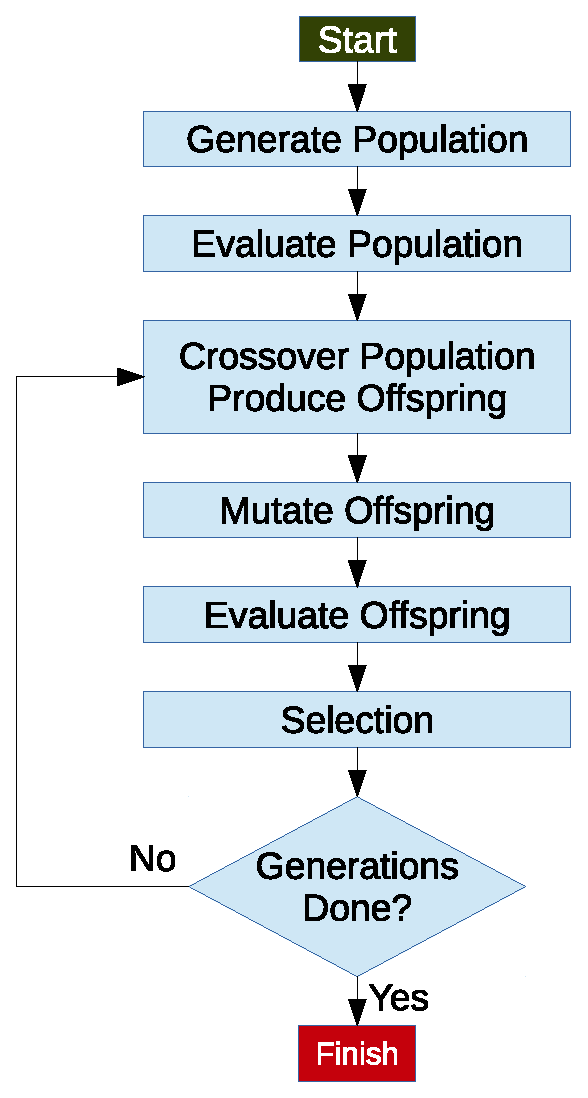
\includegraphics[width=0.5\textwidth]{ga_flowchart_background}
\caption[B\"{a}ck Simple Genetic Algorithm]{A simple genetic algorithm proposed by B\"{a}ck~\cite{Baeck2000-co}. This algorithm builds a population and then evaluates it. Next, it uses crossover to produce a pool of offspring and then mutates and evaluates the offspring. The best individuals are selected and this process is repeated until the specified number of generations are met.}
\label{fig:ga_flowchart_background}
\end{figure}

\section{Chemical Reaction Networks}
Portions of this section are borrowed from~\cite{Moles2014-ia}. The systems we use to model chemistry are known as \acrfullpl{crn}, which is an instance of an \acrfull{ac}~\cite{Dittrich2001-rn}. \Glspl{crn} give us a mean to model a set of chemical species and the way in which they react with each other to form new products. We model the chemistries by using several observations of nature, such as chemical kinetics and the law of conservation of mass. 

A \gls{crn} consists of a set of species and reactions with associated rates. In our system, molecular species are symbolic and unstructured, and there is no notion of space because we assume the solution is well stirred. In other words, the concentration of a given species is uniform throughout the solution and not unequally distributed. Actually, we do not need to handle the position of individual molecules, but rather transform all molecules of the same type (species) using rates generated by kinetic laws: mass-action~\cite{Horn1972-ob}~\cite{Erdi1989-ll} for regular and Michaelis\hyph Menten~\cite{Henri1903-jf}~\cite{Michaelis1913-zv}~\cite{Leskovac2003-ei} for catalytic reactions.

Dittrich~\cite{Dittrich2001-rn} describes an \gls{ac} made up of a finite set of molecular species and a finite set of reactions. The set of molecular species are represented by symbols. For example, the symbols representing the two reactants and products in our chemical example here are $S_1$, $S_2$, and $P$, respectively. The reactions are formed through multiple sets of species (reaction left side) that react to form products (reaction right side)~\cite{Banda2013-zs}. A reaction looks like $S_1 + S_2 \rightarrow P$ where reactants $S_1$ and $S_2$ form the product $P$.

We combine mass action kinetics with the ideas of \gls{ac} to express reaction rates for ordinary (non-catalytic) reactions. Epstein~\cite{Epstein1998-qw} expresses this through a series of differential equations. Given a generic chemical reaction $aS_1 + bS_2 \rightarrow cP$, the rate of reaction, $v$, is expressed by
\begin{equation}
v = -\frac{1}{a}\frac{d[S_1]}{dt} = -\frac{1}{b}\frac{d[S_2]}{dt} = \frac{1}{c}\frac{d[P]}{dt} = k[S_1]^a[S_2]^b,
\end{equation}
where $[S_1]$, $[S_2]$, and $[P]$ are the concentrations of the reactants, $S_1$ and $S_2$, and the product, $P$. Symbols $a$ and $b$ are stoichiometric constants, and $k$ is the reaction rate constant. Reactions could also be reversible, but in this paper, for simplification, we assume the reverse rate is always zero.

Michaelis-Menten kinetics describes the rate of a catalytic reaction where a substrate ($S$) is transformed into a product ($P$) through the use of an enzyme or catalyst ($E$) in a reaction modeled as $E + S \rightleftharpoons ES \rightarrow E + P$. The catalyst $E$ speeds up the rate of the reaction without being consumed in the process. The rate of a catalytic reaction is defined by
\begin{equation}
v = \frac{k_{cat}[E][S]}{K_m+[S]},
\end{equation}
where $k_{cat}$ and $K_m$ are rate constants~\cite{Copeland2004-sq}.

The simulations of \glspl{crn} were performed with \acrfull{coel}. \Gls{coel} is a tool developed by Banda \textit{et al.} that allows the simulation and evolution of \glspl{crn} using \glspl{ga}~\cite{Banda2014-qw}. The chemical simulations, as we will show later, take a longer period of time to run than a non-\gls{crn} simulation so distribution of the work across a \gls{hpc} cluster allows the simulations to execute faster. We have confidence in the results produced with multiple papers being published using the same tool. Building blocks, like perceptrons and \glspl{ann} as chemistries are also already modeled in \gls{coel}.

Various models of perceptrons that are constructed in a \glspl{crn} already exist. Banda \textit{et al.} have presented multiple models of the preceptron such as the \gls{asp}~\cite{Banda2014-bp} and \gls{aasp}~\cite{Banda2014-kg}. These two models of perceptrons both have a definition that allows direct mapping to a biological implementation. The \gls{aasp} is an improved version of the \gls{asp} that offers greater precision with a fewer number of reactions. Blount \textit{et al.} has shown that more than one of these pereceptrons, forming an \gls{ann}, in the same chemistry are possible with the use of chemical compartments~\cite{Blount_undated-ro}.

These chemical compartments are a means to isolate the reaction of a series of reactions from another set of reactions. From a modularity perspective, they also allow some sense of recursion by re-using the same species and reactions set by inserting multiple copies of the same compartment. Blount's compartments use a membrane to control the flow of interactions between each of the layers of an \gls{ann}. This gives way to allow multiple perceptrons to co-exist in the same solution without interfering with the processing of another perceptron. Now, in the next chapter, we will discuss the implementation of two different models of the delay line as a \gls{crn}.

  

\glsresetall
\chapter{Delay Line}
\label{chap:delay_line}
\pgfplotscreateplotcyclelist{custom list}{%
Dark2-8-1,
Dark2-8-2,
Dark2-8-3,
Dark2-8-4,
Dark2-8-5,
Dark2-8-6,
Dark2-8-7,
Dark2-8-8,
Set1-9-1,
Set1-9-2,
Set1-9-3,
Set1-9-4,
Set1-9-5,
Set1-9-6,
Set1-9-7,
Set1-9-8,
Set1-9-9}

With the knowledge of \glspl{crn} and \gls{ga}, we now move on to discuss the two models of delay line implemented as a \gls{crn}. First, a model of the delay line that has greater precision, but requires more control signals. Then, the second model requires fewer control signals, but it comes at the cost of precision. Both models are then connected with a \gls{asp} to demonstrate functionality and modularity. This chapter is based off our accepted paper~\cite{Moles2014-ia}.

\section{Delay Line Concept}

A delay line is a way to store data in an ordered fashion over time. The delay line we design operates similar to a \gls{fifo} data buffer, but allows random access to any element of the \gls{fifo}. Figure~\ref{fig:delay_line_general} shows an example of a delay line shifting values down. Table~\ref{tab:delay_line_general} shows an example of how values shift down with increasing time, $t$.

\begin{figure}
    \centering
    \begin{tikzpicture}
        [c1/.style={circle,draw=black!50,fill=Accent-4-1,thick},
         b1/.style={rectangle,draw=black!50,fill=Accent-4-2,thick},
         b2/.style={rectangle,draw=white!50,fill=white!50,thick}]
        \node[c1]    (cirt0)        {x};
        \node[b1]    (boxt0)        [right=of cirt0]        {$x(t)$}
            edge[<-]    (cirt0);
        \node[b1]    (boxt1)        [right=0.2cm of boxt0]    {$x(t-1)$}
            edge[<-]    (boxt0);
        \node[b1]    (boxt2)        [right=0.2cm of boxt1]    {$x(t-2)$}
            edge[<-]    (boxt1);
        \node[b2]    (boxte)        [right=0.2cm of boxt2]    {\ldots}
            edge[<-]    (boxt2);
        \node[b1]    (boxtn)        [right=0.2cm of boxte]    {$x(t-n)$}
            edge[<-]    (boxte);
    \end{tikzpicture}
    \caption[Delay Line]{Diagram of an example delay line. The circle, $x$, is the input value and box $x(t)$ represents the value of $x$ at current time step. Box labeled $x(t-1)$ represents one time step ago, $x(t-2)$ represents two time steps ago, and so on.}
    \label{fig:delay_line_general}
\end{figure}
    
\begin{table}
    \centering
    \begin{tabular}{l|l|l l l l}
    \textbf{t} & $\mathbf{x}$ & $\mathbf{x(t)}$ & $\mathbf{x(t-1)}$ & $\mathbf{x(t-2)}$ & $\mathbf{x(t-3)}$ \\ \hline
    0 & 15 & 15 & ~  & ~  & ~  \\
    1 & 19 & 19 & 15 & ~  & ~  \\
    2 & 12 & 12 & 19 & 15 & ~  \\
    3 & 14 & 14 & 12 & 19 & 15 \\
    4 & 11 & 11 & 14 & 12 & 19 \\
    \end{tabular}
    \caption[Delay Line Values Over Time]{Table of values for a given input value, $x$, and how they shift through a delay line. Each value, $t-n$, represents the value $n$ time steps ago.}
    \label{tab:delay_line_general}
\end{table}

\section{Delay Line Design}
\label{sec:delayline}
To introduce the time delay line design, we will first examine a delay line constructed of only two stages in two different styles. One is a \acrfull{mdl} that requires experimenter participation to indicate when it is time to move values between stages. The second model automatically propagates the signaling species backwards, hence it is more autonomous, but it comes at the cost of additional and cumulative error in the resulting output values.

\subsection{Manual Copy Delay Line}
First, we will introduce the delay line of two stages with manual copy of the signaling species shown in Figure~\ref{fig:manualprop_n_2}. A delay line of two stages is composed of seven species: $X$, $X1C$, $X1$, $X2$, $X2C$, $X2_{signal}$, and $X1_{signal}$. The species $X$ represents the input value of the delay line. The signaling species, $X1_{signal}$ and $X2_{signal}$, are the catalysts that start the reaction conversion of $X$ into corresponding stages. The primary function of $X1_{signal}$ is to trigger and accelerate the copy reaction which converts of $X$ to $X1C$ and $X1$. Species $X2_{signal}$ performs a similar action for the conversion of $X1C$ to $X2$.

Species $X1C$ and $X2C$ are delayed copies of $X$ that move to the next stage of the system (for example, $X1$ to $X2$ and $X2C$). Species $X2C$ is shown for completeness and is used to cascade the system to a delay line of more than two stages. For a two stage delay line, $X2C$ is waste and flushed. The outputs of the system are the $X1$ and $X2$ species, i.e., $X1$ and $X2$ represent the current and previous values of $X$ that are consumed as the inputs of another system.

\newsavebox\syringebox
\begin{lrbox}{\syringebox}
    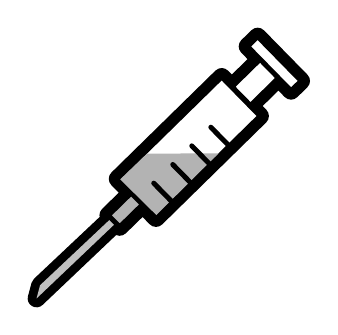
\begin{tikzpicture}[y=0.80pt, x=0.8pt,yscale=-1, inner sep=0pt, outer sep=0pt]
  \path[draw=black,fill=cc0c0c0,line join=round,line cap=round,miter
    limit=4.00,even odd rule,line width=6.400pt] (104.8628,4.3331) --
    (100.3003,8.8018) -- (105.9566,14.5831) -- (93.3003,27.0206) --
    (101.6128,35.5206) -- (114.3003,23.0831) -- (119.9566,28.8643) --
    (124.5191,24.3956) -- (104.8628,4.3331) -- cycle(88.6441,22.5518) --
    (41.6128,68.6143) -- (58.9566,86.3331) -- (105.9566,40.2393) --
    (88.6441,22.5518) -- cycle(47.7378,74.9581) -- (37.3941,85.0831) --
    (38.7066,86.4268) -- (6.5816,116.6768) -- (4.9878,122.6456) --
    (40.8316,88.5831) -- (42.5503,90.3331) -- (52.8941,80.2393) --
    (47.7378,74.9581) -- cycle;
\begin{scope}[shift={(183.219,-198.691)}]
  \path[shift={(-183.219,198.691)},fill=cc0c0c0,line join=miter,line
    cap=butt,miter limit=4.00,even odd rule,line width=2.400pt] (39.3665,85.8168)
    -- (6.5814,116.6794) -- (4.9851,122.6552) -- (41.4219,87.9924) --
    (39.3665,85.8168) -- cycle;
  \path[cm={{0.69985,0.71429,-0.71429,0.69985,(-183.219,198.691)}},draw=black,fill=cffffff,line
    join=round,line cap=round,miter limit=4.00,nonzero rule,line
    width=1.805pt,rounded corners=0.0000cm] (78.1378,-47.5230) rectangle
    (102.9168,18.3064);
  \path[cm={{0.69985,0.71429,-0.71429,0.69985,(-183.219,198.691)}},draw=black,fill=cffffff,line
    join=round,line cap=round,miter limit=4.00,nonzero rule,line
    width=1.805pt,rounded corners=0.0000cm] (84.5786,-71.0885) rectangle
    (96.4759,-47.7304);
  \path[cm={{0.69985,0.71429,-0.71429,0.69985,(-183.219,198.691)}},draw=black,fill=cffffff,line
    join=round,line cap=round,miter limit=4.00,nonzero rule,line
    width=1.805pt,rounded corners=0.0000cm] (76.4862,-71.8876) rectangle
    (104.5683,-65.4768);
  \path[cm={{0.69985,0.71429,-0.71429,0.69985,(-183.219,198.691)}},draw=black,fill=cb3b3b3,line
    join=round,line cap=round,miter limit=4.00,nonzero rule,line
    width=1.805pt,rounded corners=0.0000cm] (86.9479,18.3706) rectangle
    (94.3150,32.8346);
  \path[fill=cb3b3b3,line join=round,line cap=round,miter limit=4.00,nonzero
    rule,line width=1.645pt] (-128.3155,255.9149) -- (-96.0548,255.7926) --
    (-124.1199,283.6438) -- (-140.4350,267.5587) -- (-128.3155,255.9149) -- cycle;
  \path[shift={(-183.219,198.691)},draw=black,fill=c00ffff,line join=round,line
    cap=round,miter limit=4.00,even odd rule,line width=1.805pt] (65.9531,78.7460)
    .. controls (57.7865,70.4108) and (57.9323,70.5597) .. (57.9323,70.5597);
  \path[shift={(-183.219,198.691)},draw=black,fill=c00ffff,line join=round,line
    cap=round,miter limit=4.00,even odd rule,line width=1.805pt] (74.5488,70.3242)
    .. controls (66.3821,61.9890) and (66.5280,62.1378) .. (66.5280,62.1378);
  \path[shift={(-183.219,198.691)},draw=black,fill=c00ffff,line join=round,line
    cap=round,miter limit=4.00,even odd rule,line width=1.805pt] (83.1444,61.9023)
    .. controls (74.9777,53.5671) and (75.1236,53.7160) .. (75.1236,53.7160);
  \path[shift={(-183.219,198.691)},draw=black,fill=c00ffff,line join=round,line
    cap=round,miter limit=4.00,even odd rule,line width=1.805pt] (91.7400,53.4804)
    .. controls (83.5734,45.1453) and (83.7192,45.2941) .. (83.7192,45.2941);
\end{scope}

\end{tikzpicture}


\end{lrbox}

\newcommand \syringePDFImage{\usebox\syringebox}

\begin{figure}[ht]
	\centering
	\begin{tikzpicture}
		[t1/.style={circle,draw=black!100,fill=Accent-4-1,thick},
		 tsig/.style={circle,draw=black!100,fill=Accent-4-1,thick},
		 t2/.style={circle,draw=black!100,fill=Accent-4-2,thick},
		 t3/.style={circle,draw=black!100,fill=Accent-4-3},
		 lmb/.style={circle,draw=white!100,fill=white!50}]

		\node[t1]	(xinj)		{$X$};
		\node[t2]	(x1)		[below right=of xinj]	{$X1$};
		\node[t3]	(x1c)		[below left=of xinj]	{$X1C$};
		\node[t2]	(x2)		[below right=of x1c]	{$X2$};
		\node[t3]	(x2c)		[below left=of x1c]		{$X2C$};
		\node[tsig]	(x2sig)		[left=of x1c]			{$X2_{signal}$};
		\node[tsig] (x1sig)     [left=of xinj]			{$X1_{signal}$};
		\node[lmb]  (lamb)		[above=of x1sig]		{$\lambda$};
		\node[lmb]  (lamb2)		[above=of x2sig]		{$\lambda$};

		\node[scale=0.2]	(syr1)		[above right=-0.1cm of xinj]	{\syringePDFImage};
		\node[scale=0.2,rotate=90]	(syr2)		[above left=0.1cm of x2sig]	{\syringePDFImage};
		\node[scale=0.2,rotate=90]	(syr3)		[above left=0.1cm of x1sig]	{\syringePDFImage};

		\draw[->,thick] (xinj.south) -- ($(x1c.north)!0.5!(x1.north)$) to[out=-90,in=0] (x1c.east);
		\draw[->,thick] (xinj.south) -- ($(x1c.north)!0.5!(x1.north)$) to[out=-90,in=180] (x1.west);

		\draw[->,thick] (x1c.south) -- ($(x2c.north)!0.5!(x2.north)$) to[out=-90,in=0] (x2c.east);
		\draw[->,thick] (x1c.south) -- ($(x2c.north)!0.5!(x2.north)$) to[out=-90,in=180] (x2.west);

		\draw[->,dashed,thick] (x1sig.south east) -- ($(x1c.north)!0.5!(x1.north)$);
		\draw[->,dashed,thick] (x2sig.south east) -- ($(x2c.north)!0.5!(x2.north)$);

		\draw[->,thick] (x2sig.north) to[out=90,in=270] (lamb2.south);
		\draw[->,thick] (x1sig.north) to[out=90,in=270] (lamb.south);

	\end{tikzpicture}
	\caption[Two Stage Manual Copy Delay Line]{\Gls{mdl} with two stages. The syringe is used to indicate the species where inputs are presented and $X1$ and $X2$ represent the output species from the delay line. Species $X2C$ is used to cascade a value to a delay line of greater than two stages. The signal species, $X1_{signal}$ and $X2_{signal}$, catalyze the copy reactions and are removed from the system by decay ($\lambda$).}
	\label{fig:manualprop_n_2}
\end{figure}

Species $X1C$ is the internal transition storage species. The storage species acts as a buffer for the value that will transition into $X2$ on next activation of the system with an $X2_{signal}$ passed in. Ideally, the concentration of $X1C$ will be the same as $X1$ prior to its consumption. This process is represented by a set of reactions using the previously mentioned species. Reactions~\ref{eq:XreacMan}~and~\ref{eq:X1CreacMan} (below) represent the conversion of the input species, $X$, through to the output species, $X1$ and $X2$.
\begin{alignat}{2}
X & \xrightarrow{X1_{signal}} & X1 + X1C  \label{eq:XreacMan} \\
X1C & \xrightarrow{X2_{signal}} & X2 + X2C \label{eq:X1CreacMan}
\end{alignat}
Reactions~\ref{eq:X2sigMan} and \ref{eq:X1sigMan} show the decay (represented by lambda, $\lambda$) of the catalyst species, $X1_{signal}$ and $X2_{signal}$.
\begin{alignat}{2}
X2_{signal} & \rightarrow & \lambda \label{eq:X2sigMan} \\
X1_{signal} & \rightarrow & \lambda \label{eq:X1sigMan}
\end{alignat}

Now, using these reactions, we can examine data moving through the delay line. For this \gls{mdl}, actions must occur at two moments (in time). First, at time zero, we present a random value to the input $X$ and reset $X1$ and $X2$ to zero. The reset of $X1$ and $X2$ simulate consumption by the underlying system the delay line is integrated with. Species $X2_{signal}$ is set to one to copy the value stored in $X1C$ to $X2$. In the ideal case for the initialization and first run of the delay line, $X2$ should be zero until these actions repeat. After 25 time steps, $X1_{signal}$ is injected to the system. The wait is to fully allow the transition of $X1C$ to $X2$ before beginning the transformation of $X$ to $X1C$. These injections repeat every 1,000 time steps and are summarized in Table~\ref{tab:as2Man}. Table~\ref{tab:as2Pipeline} shows an example of these injections repeating every 1,000 time steps with example data moving through.

\begin{table}[ht]
	\caption[Two Stage Manual Delay Line Actions]{Actions for two stage \gls{mdl} simulations.}
	\label{tab:as2Man}
	\centering
	\begin{tabular}{lll}
		Time		& Species			& Value 					\\ \hline
		0			& $X$				& $0.0 \le rand() \le 1.0$	\\
		0			& $X1$				& 0							\\
		0			& $X2$				& 0							\\
		0			& $X2_{Signal}$ 	& 1							\\
		25			& $X1_{Signal}$ 	& 1							\\
	\end{tabular}
\end{table}

\begin{table}
	\centering
	\caption[Pipeline View of Data in Two Stage Manual Delay Line]{Pipeline view of data moving through manual signaling delay line from Table~\ref{tab:as2Man}. Bold items show those injected to the system. \textbf{A}, \textbf{B}, and \textbf{C} are inputs and \textbf{1} is a concentration (presence) of $Xm_{signal}$.}
	\label{tab:as2Pipeline}
    \begin{tabular}{l|l|l|l|l|l|l}
    Species  & Time=0                     & 25                         & 1000                       & 1025                       & 2000                       & 2025                       \\ \hline
    X        & $\textbf{A}$               & $A \rightarrow 0$          & $\textbf{B}$               & $B \rightarrow 0$          & $\textbf{C}$               & $C \rightarrow 0$          \\
    X1signal & ~                          & $\textbf{1} \rightarrow 0$ & ~                          & $\textbf{1} \rightarrow 0$ & ~                          & $\textbf{1} \rightarrow 0$ \\
    X2signal & $\textbf{1} \rightarrow 0$ & ~                          & $\textbf{1} \rightarrow 0$ & ~                          & $\textbf{1} \rightarrow 0$ & ~                          \\ \hline
    X1       & $\textbf{0}$               & $0 \rightarrow A$          & $\textbf{0}$               & $0 \rightarrow B$          & $\textbf{0}$               & $0 \rightarrow C$          \\
    X1C      & ~                          & $\rightarrow A$            & $A \rightarrow 0$          & $0 \rightarrow B$          & $B \rightarrow 0$          & $0 \rightarrow C$          \\
    X2       & $\textbf{0}$               & ~                          & $\textbf{0} \rightarrow A$ & $A$                        & $\textbf{0} \rightarrow B$ & $B$                        \\
    X2C      & ~                          & ~                          & $\rightarrow A$            & $A$                        & $A \rightarrow B$          & $B$                        \\
    \end{tabular}
\end{table}

Figures~\ref{fig:delay2allMan_A} and ~\ref{fig:delay2allMan_B} shows the results of running the actions in Table~\ref{tab:as2Man} for 10 iterations (10,000 time steps). Valid data is available for examination on output species $X1$ and $X2$ every time steps after each cycle. Figure~\ref{fig:delay2XMan} shows the input values injected to the manual delay line. During the first cycle, species $X2$ remains at zero since there is no previous value as seen in Figure~\ref{fig:delay2X1Man}. Figure~\ref{fig:delay2X2SignalMan} shows the catalysts, $X2_{signal}$ and $X1_{signal}$, sequentially injected each cycle. Figure~\ref{fig:delay2X2SignalZoomedMan} presents the sequence of actions where $X2_{signal}$ is injected at time zero followed by $X1_{signal}$ 25 time steps later.

\begin{figure}[ht]
	\centering
	\begin{subfigure}[b]{0.9\textwidth}
	    \centering
		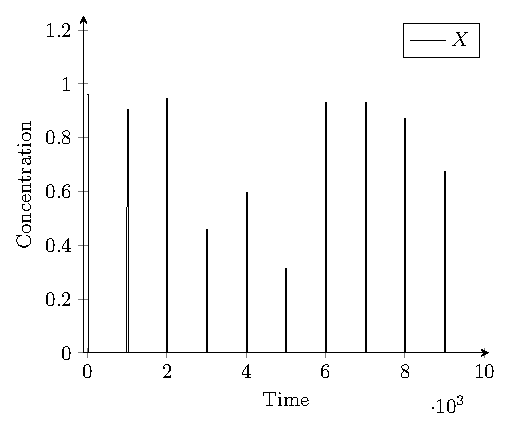
\includegraphics[width=9cm]{ac_3505_as_1979_t_10000_x1Inj}
		\caption{Input}
		\label{fig:delay2XMan}
		\vspace{15mm}
	\end{subfigure}
	\\
	\begin{subfigure}[b]{0.9\textwidth}
	    \centering
		\includegraphics[width=9cm]{ac_3505_as_1979_t_10000_x1_x2}
		\caption{Outputs}
		\label{fig:delay2X1Man}
	\end{subfigure}
	\caption[Two Stage Manual Copy Delay Line I/O]{Two stage \gls{mdl} showing input and output signals. Data arrives as input (\ref{fig:delay2XMan}) and is available on outputs (\ref{fig:delay2X1Man}) with $X1$ being the current and $X2$ being the previous $X$.}
	\label{fig:delay2allMan_A}
\end{figure}

\begin{figure}[ht]
    \centering
	\begin{subfigure}[b]{0.9\textwidth}
	    \centering
		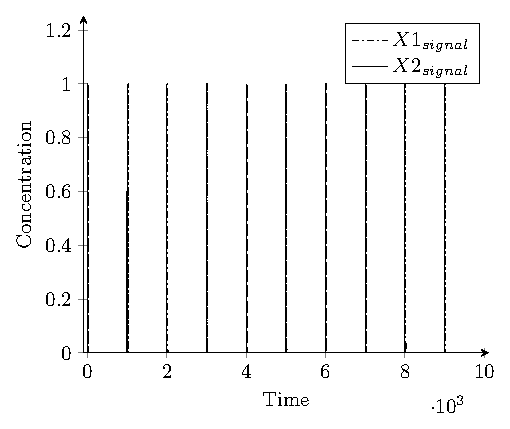
\includegraphics[width=9cm]{ac_3505_as_1979_t_10000_x1signal_x2signal}
		\caption{Copy Signals}
		\label{fig:delay2X2SignalMan}
		\vspace{15mm}
	\end{subfigure}
	\\
	\begin{subfigure}[b]{0.9\textwidth}
	    \centering
		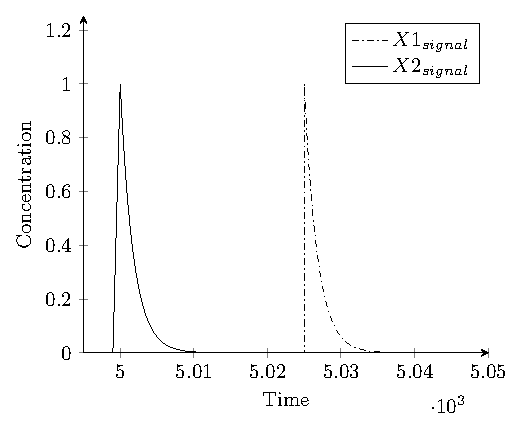
\includegraphics[width=9cm]{ac_3505_as_1979_t_10000_x1signal_x2signal_zoomed}
		\caption{Copy Signals (Zoomed on Figure~\ref{fig:delay2X2SignalMan})}
		\label{fig:delay2X2SignalZoomedMan}
	\end{subfigure}
	\caption[Two Stage Manual Copy Delay Line Signaling]{Two stage \gls{mdl} showing the copy signals. The copy of this data is triggered by $X1_{signal}$ and $X2_{signal}$ (\ref{fig:delay2X2SignalMan}). Figure~\ref{fig:delay2X2SignalZoomedMan} shows the copy signals zoomed in from Figure~\ref{fig:delay2X2SignalMan}.}
	\label{fig:delay2allMan_B}
\end{figure}

\subsection{Backwards Signal Propagation Delay Line}
The \acrfull{bpl} handles the signal species differently. More specifically, the only input signaling species is $X2_{signal}$ and rather than decay, $X2_{signal}$ reacts to $X1_{signal}$. The advantage of this model is that the user is only required to perform actions at the beginning of the cycle and then the system transforms the species internally (without external help). Figure~\ref{fig:delayelement} shows a revision of the \gls{mdl} for this model. This reduces the number of injections to two: the input ($X$) and the final copy signal ($X2_{signal}$ for two stage). The change leaves reactions~\ref{eq:Xreac} and \ref{eq:X1Creac} unchanged.

\begin{figure}[ht]
	\centering
	\begin{tikzpicture}
		[t1/.style={circle,draw=black!100,fill=Accent-4-1,thick},
		 tsig/.style={circle,draw=black!100,fill=Accent-4-1,thick},
		 t2/.style={circle,draw=black!100,fill=Accent-4-2,thick},
		 t3/.style={circle,draw=black!100,fill=Accent-4-3},
		 lmb/.style={circle,draw=white!100,fill=white!50}]

		\node[t1]	(xinj)		{$X$};
		\node[t2]	(x1)		[below right=of xinj]	{$X1$};
		\node[t3]	(x1c)		[below left=of xinj]	{$X1C$};
		\node[t2]	(x2)		[below right=of x1c]	{$X2$};
		\node[t3]	(x2c)		[below left=of x1c]		{$X2C$};
		\node[tsig]	(x2sig)		[left=of x1c]			{$X2_{signal}$};
		\node[tsig] (x1sig)     [left=of xinj]			{$X1_{signal}$};
		\node[lmb]  (lamb)		[above=of x1sig]		{$\lambda$};			

		\node[scale=0.2]	(syr1)		[above right=-0.1cm of xinj]	{\syringePDFImage};
		\node[scale=0.2,rotate=90]	(syr2)		[above left=0.1cm of x2sig]	{\syringePDFImage};

		\draw[->,thick] (xinj.south) -- ($(x1c.north)!0.5!(x1.north)$) to[out=-90,in=0] (x1c.east);
		\draw[->,thick] (xinj.south) -- ($(x1c.north)!0.5!(x1.north)$) to[out=-90,in=180] (x1.west);

		\draw[->,thick] (x1c.south) -- ($(x2c.north)!0.5!(x2.north)$) to[out=-90,in=0] (x2c.east);
		\draw[->,thick] (x1c.south) -- ($(x2c.north)!0.5!(x2.north)$) to[out=-90,in=180] (x2.west);

		\draw[->,dashed,thick] (x1sig.south east) -- ($(x1c.north)!0.5!(x1.north)$);
		\draw[->,dashed,thick] (x2sig.south east) -- ($(x2c.north)!0.5!(x2.north)$);

		\draw[->,thick] (x2sig.north) to[out=90,in=180] (x1sig.west);
		\draw[->,thick] (x1sig.north) to[out=90,in=270] (lamb.south);

	\end{tikzpicture}
	\caption[Two Stage Backwards Propagating Delay Line]{Backwards propagating delay design with two stages. The syringe is used to indicate an injection of the input species $X$ and the copy signal $X2_{signal}$. The species $X1$ and $X1$ represent the output species from the delay line. The signal $X2_{signal}$ is propagated backwards to $X1_{signal}$ without user intervention and then decays ($\lambda$).}
	\label{fig:delayelement}
\end{figure}

\begin{alignat}{2}
X & \xrightarrow{X1_{signal}} & X1 + X1C  \label{eq:Xreac} \\
X1C & \xrightarrow{X2_{signal}} & X2 + X2C\label{eq:X1Creac}
\end{alignat}

Revising the remaining reactions requires modifying only reaction~\ref{eq:X2sigMan}. Removing the decay from reaction~\ref{eq:X2sigMan} so that $X2_{signal}$ reacts to $X1_{signal}$ gives the updated reactions~\ref{eq:X2sig} and \ref{eq:X1sig}.

\begin{alignat}{2}
X2_{signal} & \rightarrow & X1_{signal} \label{eq:X2sig} \\
X1_{signal} & \rightarrow & \lambda \label{eq:X1sig}
\end{alignat}

All actions in the system occur instantaneously and are the same as actions employed by the manual delay line at time zero. At the beginning of every cycle, $X1$ and $X2$ are set to zero to simulate the next block of the system consuming their values. Also, a random value ($X$) and signal ($X2_{signal}$) are injected to the system. Table~\ref{tab:as2} summarizes these actions, which repeat every 1,000 time steps to ensure enough time for all reactions to reach steady state.

\begin{table}
	\caption[Two Stage Backwards Propagation Delay Line]{Actions for two stage back propagation delay line simulations. These actions repeat every 1000 similar to Table~\ref{tab:as2Pipeline}.}
	\label{tab:as2}
	\centering
	\begin{tabular}{lll}
		Time		& Species			& Value 					\\ \hline
		0			& $X$				& $0.0 \le rand() \le 1.0$	\\
		0			& $X1$				& 0							\\
		0			& $X2$				& 0							\\
		0			& $X2_{Signal}$ 	& 1							\\
	\end{tabular}
\end{table}

The simulations of the \gls{bpl} run for 10,000 time steps (same as for the manual delay line). Valid data is also produced at the same point (every 50 steps) on the output species $X1$ and $X2$. The value produced on the first cycle of $X2$ ideally should be zero, but leakage from $X1C$ is generally seen from steps zero to 1,000 (see Figure~\ref{fig:delay2X1}). An input is introduced to the system at species $X$ (Figure~\ref{fig:delay2X}) and then is reacted in the same cycle to species $X1$ (Figure~\ref{fig:delay2X1}). After the next cycle (i.e., the next introduction of $X2_{signal}$), the value injected at $X$ previously is now presented at $X2$ (Figure~\ref{fig:delay2X1}).

Notice that the backwards propagation introduces an error to the system with some of the $X2$ values not lining up exactly with the previous $X1$. This difference is due to the time window that the reactions for $X$ to $X1$ and $X1$ to $X2$ are simultaneously active. Looking at Figure~\ref{fig:delay2X2SignalZoomed}, $X1_{signal}$ and $X2_{signal}$ are large enough for both catalyses to occur. So, for this small window of time, there is effectively a direct path from $X$ to cascade down to $X2$. This overlap is not inherently a problem. It allows the desired parallelism of this system. We can afford this error in a small number of stages, but the inaccuracy can grow with a larger number of stages.

\begin{figure}[ht]
	\centering
	\begin{subfigure}[b]{0.9\textwidth}
	    \centering
		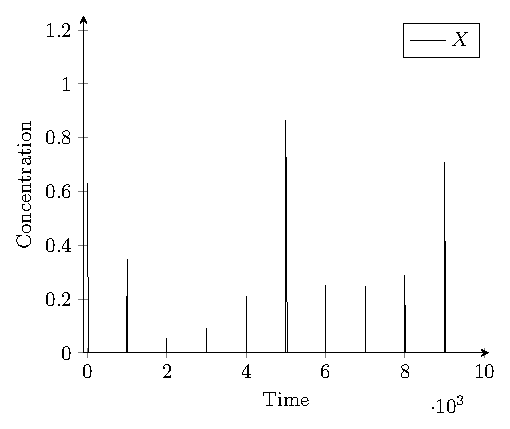
\includegraphics[width=9cm]{ac_3502_as_1957_t_10000_x1Inj}
		\caption{Input}
		\label{fig:delay2X}
		\vspace{15mm}
	\end{subfigure}
	\\
	\begin{subfigure}[b]{0.9\textwidth}
	    \centering
		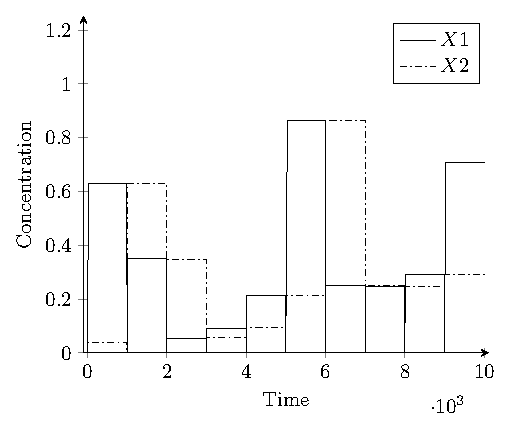
\includegraphics[width=9cm]{ac_3502_as_1957_t_10000_x1_x2}
		\caption{Outputs}
		\label{fig:delay2X1}
	\end{subfigure}
	\caption[Two Stage Backwards Propagating Delay Line I/O]{Two stage backwards propagation delay line showing inputs and outputs. Data arrives as input (\ref{fig:delay2X}) and is available on outputs (\ref{fig:delay2X1}) with $X1$ being the current and $X2$ being the previous $X$.}
	\label{fig:delay2all_A}
\end{figure}

\begin{figure}[ht]
    \centering
	\begin{subfigure}[b]{0.9\textwidth}
	    \centering
		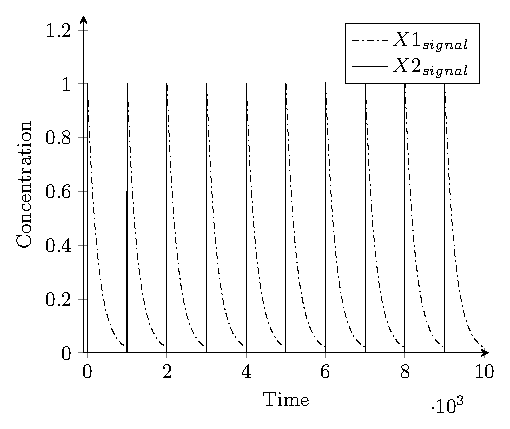
\includegraphics[width=9cm]{ac_3502_as_1957_t_10000_x1signal_x2signal}
		\caption{Copy Signals}
		\label{fig:delay2X2Signal}
		\vspace{15mm}
	\end{subfigure}
	\\
	\begin{subfigure}[b]{0.9\textwidth}
	    \centering
		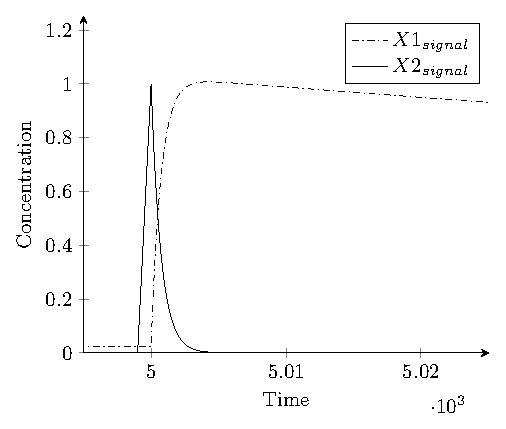
\includegraphics[width=9cm]{ac_3502_as_1957_t_10000_x1signal_x2signal_zoomed}
		\caption{Copy Signals (Zoomed on Figure~\ref{fig:delay2X2Signal})}
		\label{fig:delay2X2SignalZoomed}
	\end{subfigure}
	\caption[Two Stage Backwards Propagating Delay Line Signaling]{Two stage backwards propagation delay line showing copy signaling. The copy is started by $X1_{signal}$ and $X2_{signal}$ (\ref{fig:delay2X2Signal}). Figure~\ref{fig:delay2X2SignalZoomed} shows the signals controlling propagation zoomed in from Figure~\ref{fig:delay2X2Signal}.}
	\label{fig:delay2all_B}
\end{figure}

\subsection{Inherit Single Instruction, Multiple Data}
With the nature of chemistry, one of the advantages of our unconventional delay line implementation is the ability to perform single instruction, multiple data~\cite{Flynn1972-sd} operations. The main factor is finding a unique set of species to hold each delay line that will not react with surrounding buffers to allow such parallel operations. Figure~\ref{fig:simd} shows an example of a two-stage set of backwards propagation and \glspl{mdl} that are producing a vector of three values for the current and previous cycles.

\begin{figure}[ht]
	\centering
		\begin{tikzpicture}
		[inp/.style={rectangle,draw=black!75,fill=Accent-4-1,thick},
		 delay/.style={rectangle,draw=black!100,fill=Accent-4-2,thick,align=left},
		 res/.style={rectangle,draw=white!0,fill=white!20,thick,align=left}]

		\node[inp] 		(input)								{$X2_{signal}$};
		\node[delay]	(delay1)	[right=of input]		{2-stage BPDL};
		\node[delay]	(delay2)	[below=of delay1]		{2-stage BPDL};
		\node[delay]	(delay3)	[below=of delay2]		{2-stage MCDL};

		\node[res]		(res1)		[right=of delay1]		{$X[0][0]$ \\ $X[-1][0]$};
		\node[res]		(res2)		[right=of delay2]		{$X[0][1]$ \\ $X[-1][1]$};
		\node[res]		(res3)		[right=of delay3]		{$X[0][2]$ \\ $X[-1][2]$};

		\node[inner sep = 0, minimum size = 0] (k) at ($(input.east)!0.5!(delay1.west)$) {};


		\draw[->,thick] (input.east) -- (k) |- (delay1.west);
		\draw[->,thick] (input.east) -- (k) |- (delay2.west);
		\draw[->,thick] (input.east) -- (k) |- (delay3.west);

		\draw[->,thick] (delay1.east) -- (res1.west);
		\draw[->,thick] (delay2.east) -- (res2.west);
		\draw[->,thick] (delay3.east) -- (res3.west);
	\end{tikzpicture}
	\caption[Single Instruction, Multiple Data Representation with Delay Line]{Time delay design \gls{simd} representation showing simultaneous output of previous ($X[-1][n]$) and current ($X[0][n]$) $X$ for parallel data processing. The signaling can be used with multiple instances of a delay line, both for the manual copy and the back propagation type.}
	\label{fig:simd}
\end{figure}

\subsection{More than Two Stages}
Extending the buffer for more than two stages is straightforward. For each stage we add one output species ($Xm$), transition species ($XmC$), and catalyst species ($Xm_{signal}$). This allows the system to flexibly provide a buffer of desired length. As an example, Figure~\ref{fig:delayelement3} shows a \gls{bpl} with three stages. The total number of species required in the system grows at a rate of $3m+1$, where $m$ is equal to the number of stages in the system. One trade-off to note is that as the number of stages in the system increases, so does the period of time to cascade values through the delay line. Ideally, each reaction runs to full completion prior to $Xm_{signal}$ propagating backwards to begin the next conversion.

\begin{figure}[ht]
	\centering
	\begin{tikzpicture}
		[t1/.style={circle,draw=black!100,fill=Accent-4-1,thick},
		 tsig/.style={circle,draw=black!100,fill=Accent-4-1,thick},
		 t2/.style={circle,draw=black!100,fill=Accent-4-2,thick},
		 t3/.style={circle,draw=black!100,fill=Accent-4-3},
		 lmb/.style={circle,draw=white!100,fill=white!50}]

		\node[t1]	(xinj)		{$X$};
		\node[t2]	(x1)		[below right=of xinj]	{$X1$};
		\node[t3]	(x1c)		[below left=of xinj]	{$X1C$};
		\node[t2]	(x2)		[below right=of x1c]	{$X2$};
		\node[t3]	(x2c)		[below left=of x1c]		{$X2C$};
		\node[tsig]	(x2sig)		[left=of x1c]			{$X2_{signal}$};
		\node[tsig] (x1sig)     [left=of xinj]			{$X1_{signal}$};			
		\node[tsig]	(x3sig)		[left=of x2c]			{$X3_{signal}$};
		\node[t3]	(x3c)		[below left=of x2c]		{$X3C$};
		\node[t2]	(x3)		[below right=of x2c]	{$X3$};
		\node[lmb]  (lamb)		[above=of x1sig]		{$\lambda$};

		\node[scale=0.2]	(syr1)		[above right=-0.1cm of xinj]	{\syringePDFImage};
		\node[scale=0.2,rotate=90]	(syr2)		[above left=0.1cm of x3sig]	{\syringePDFImage};

		\draw[->,thick] (xinj.south) -- ($(x1c.north)!0.5!(x1.north)$) to[out=-90,in=0] (x1c.east);
		\draw[->,thick] (xinj.south) -- ($(x1c.north)!0.5!(x1.north)$) to[out=-90,in=180] (x1.west);

		\draw[->,thick] (x1c.south) -- ($(x2c.north)!0.5!(x2.north)$) to[out=-90,in=0] (x2c.east);
		\draw[->,thick] (x1c.south) -- ($(x2c.north)!0.5!(x2.north)$) to[out=-90,in=180] (x2.west);

		\draw[->,thick] (x2c.south) -- ($(x3c.north)!0.5!(x3.north)$) to[out=-90,in=180] (x3.west);
		\draw[->,thick] (x2c.south) -- ($(x3c.north)!0.5!(x3.north)$) to[out=-90,in=0] (x3c.east);

		\draw[->,dashed,thick] (x1sig.south east) -- ($(x1c.north)!0.5!(x1.north)$);
		\draw[->,dashed,thick] (x2sig.south east) -- ($(x2c.north)!0.5!(x2.north)$);
		\draw[->,dashed,thick] (x3sig.south east) -- ($(x3c.north)!0.5!(x3.north)$);

		\draw[->,thick] (x2sig.north) to[out=90,in=180] (x1sig.west);
		\draw[->,thick] (x3sig.north) to[out=90,in=180] (x2sig.west);

		\draw[->,thick] (x1sig.north) to[out=90,in=270] (lamb.south);
	\end{tikzpicture}
	\caption[Three Stage Backwards Propagating Delay Line]{\Gls{bpl} with three stages. The syringe is used to indicate an injection of the input $X$ and the signal $X3_{signal}$. Species $X1$, $X2$, and $X3$ represent the output species from the delay line. Lambda ($\lambda$) shows decay of backwards propagation signal.}
	\label{fig:delayelement3}
\end{figure}

The reaction set of the delay line also scales in a straightforward fashion. Each intermediate delay stage has a reaction similar to reaction~\ref{eq:Xreac} and the final delay stage (the $m^{th}$ delay) has a reaction similar to reaction~\ref{eq:X1Creac}. This remains true for extending both the manual and backwards propagating delay line. Extension of the catalysts depends on the implementation. For the \gls{mdl}, simply adding the species and a subsequent input is required. Extending the backward propagating delay line has the advantage that it does not increase the number of injections, but it still increases the overall number of species.

\section{Results}
\label{sec:dl_results}
We will highlight the results for the two stage buffer and its extension beyond two stages. We employed Genetic Algorithms (GAs)~\cite{Mitchell1998-tw} to optimize the rate constants (mapped to chromosomes) of the backwards propagation model. We only used the algorithm to optimize the backwards propagation model since the manual copy was straightforward to optimize by hand. The GA used an elite selection of the top 20 chromosomes from the population of 100, which undergo cross-over and mutation to form the next generation. The goal (fitness function) of this evolutionary algorithm was to minimize the error of the delay line.

We defined error as the difference between the actual input value ($X$) and the value occurring at $X1$ on this cycle and then $X2$ on the next cycle. We performed this test 50 time steps after $X$ is injected into the delay line. Equation~\ref{eq:errorequation} shows the calculation of this error where $X[n]$ represents the current value of $X$ and $X[n-1]$ represents the value of $X$ on the previous input cycle. Adding both differences for the two stage delay line provided the overall error.

\begin{equation}
error = |X_1 - X[n]| + |X_2 - X[n-1]| \label{eq:errorequation}
\end{equation}

The genetic algorithm performed perturbation mutation that changed each chromosome's element with 30\% chance by $\pm$30\% using a uniform distribution. We ran the GA for 100 generations to produce the results for the two stage delay line. The algorithm was configured to target a transition of the input species, $X$, to the current time species, $X1$, as fast as possible, and convert the intermediate species, $X1C$ to the previous time species, $X2$, as fast as possible while minimizing the amount of leakage between the phases of the design.

\subsection{Two Stages}
Table~\ref{tab:rateconstantsMan} shows the rate constants for the manual propagation delay line reactions. Rates for the conversion of input species, $X$, down the chain is the same rate with the presence of $X1_{signal}$ and $X2_{signal}$ both increasing the rate by the same amount because the forward copy reactions should be as fast as possible. Figures~\ref{fig:delay2allMan_A} and \ref{fig:delay2allMan_B} shows the plots using these rate constants in a two stage system, which can be replicated for a manual copy system of any size.

\begin{table}[ht]
    \caption[Two Stage Manual Copy Delay Line Rate Constants]{Rate constants of two stage \gls{mdl} found by GA.}
    \label{tab:rateconstantsMan}
    \centering
    \begin{tabular}{llll}
	    Reaction                                 & Forward Rate & $K_m$          \\ \hline
	    $X \xrightarrow{X1_{signal}} X1 + X1C$   & 0.0757       & 2.0000         \\
	    $X1C \xrightarrow{X2_{signal}} X2 + X2C$ & 0.0757       & 2.0000         \\
		$X2_{signal} \rightarrow \lambda$        & 0.5643       & (None)         \\
	    $X1_{signal} \rightarrow \lambda$        & 0.5643       & (None)         \\
    \end{tabular}
\end{table}

For a different size, the back propagation delay line has different rate constants. In addition, the rate constants were not grouped like the manual propagation delay line because it would drastically decrease the performance. Looking at the constants in Table~\ref{tab:rateconstants}, the reaction for species $X1C$ to $X2$ is the fastest. This is directly due to the rapid rate that $X2_{signal}$ is reacting to $X1_{signal}$. Effectively, to meet the first requirement of getting $X$ into $X1$ as fast as possible, the lower level transition of species (Reaction~\ref{eq:X1Creac}) must complete before. Figures~\ref{fig:delay2all_A} and \ref{fig:delay2all_B} shows the output of a two stage \gls{bpl} with the rate constants in Table~\ref{tab:rateconstants}.

\begin{table}
    \caption[Two Stage Backwards Propagating Delay Line Rate Constants]{Rate constants of two stage \gls{bpl} found by GA.}
    \label{tab:rateconstants}
    \centering
    \begin{tabular}{llll}
	    Reaction                                 & Forward Rate & $K_m$          \\ \hline
	    $X \xrightarrow{X1_{signal}} X1 + X1C$   & 0.0020       & 0.0225         \\
	    $X1C \xrightarrow{X2_{signal}} X2 + X2C$ & 0.0706       & 2.0000         \\
	    $X2_{signal} \rightarrow X1_{signal}$    & 1.3648       & (None)         \\
	    $X1_{signal} \rightarrow \lambda$        & 0.0039       & (None)         \\
    \end{tabular}
\end{table}

To compare the accumulated error of the two delay lines we used symmetric mean absolute percentage error (SAMP) defined as
\begin{equation}
SAMP = 100 * \langle \frac{|y-\hat{y}|}{y+\hat{y}} \rangle,
\end{equation}
where $\langle.\rangle$ is the mean of a set of multiple values, $y$ is the actual value, and $\hat{y}$ is the expected value. We calculated an average SAMP per stage (unit size) by dividing cumulative SAMP with $m$. More specifically, using $n$ to represent a discrete time series sample and $m$ to represent the number of stages:
\begin{equation}
SAMP = \frac{100}{m} * \sum \limits_{k=1}^{m} \langle \frac{|Xk-X[n-(k-1)]|}{Xk+X[n-(k-1)]} \rangle.
\end{equation}
For instance, SAMP for two stages ($m=2$) is given by
\begin{equation}
SAMP = \frac{100}{2} * \langle \frac{|X1-X[n]|}{X1+X[n]} + \frac{|X2-X[n-1]|}{X2+X[n-1]} \rangle \label{eq:sampn2}.
\end{equation}

We evaluated performance (error) over 10,000 runs, each repeating the sequence of actions defined in Table~\ref{tab:as2Man} and Table~\ref{tab:as2} for 200 iterations (200,000 time steps). Figure~\ref{fig:fiveStageAbsDiff} shows the results for a delay line of size two as well as for larger sizes (discussed in next section). The difference in values from expected values for the two stage delay line are quite small. This shows that for a two stage delay line, both types operate well. One thing to note is that the backwards delay line has a larger initial error which can accumulate over time.

\subsection{Over Two Stages}
\label{sec:dl_paper_over_two_stages}
In this section, we will examine the use of a delay line with five stages. Five stages was selected and executed for both the manual copy and back propagating delay line. Figure~\ref{fig:fiveStageAbsDiff} shows the final error when evaluated for 10,000 runs for 200 iterations each (same as for $m=2$ in previous section). The maximum error over the entire evaluation is shown in Table~\ref{tab:maxSAMP}. There are a few observations to note on this plot. The error on a backwards propagation delay line ($B$) increases as the number of stages in the delay line increases. For a smaller delay line, this error would generally be negligible, but for larger sizes this could be a concern. The manual copy has a significantly smaller error as shown in Figure~\ref{fig:fiveStageAbsDiff}.

\begin{figure}[ht]
	\centering
	\begin{tikzpicture}
		\begin{axis}[
		xlabel={Step},
		ylabel={SAMP},
		xticklabel style={/pgf/number format/fixed},
		enlargelimits=true,
		cycle multi list={Mark-Dark2-8},
		legend style={
			legend pos=outer north east,
			legend columns=1,
		},
		ymode=log,
		axis x line=bottom,
		axis y line=left,
		width=13cm,
		height=7.313cm,
		mark repeat=20,
		]
			\addplot table [x=Step, y=manual2, col sep=comma] {data/performance_back_manual.csv};
			\addplot table [x=Step, y=manual5, col sep=comma] {data/performance_back_manual.csv};
			\addplot table [x=Step, y=manual10, col sep=comma] {data/performance_back_manual.csv};

			\addplot table [x=Step, y=back2, col sep=comma] {data/performance_back_manual.csv};
			\addplot table [x=Step, y=back3, col sep=comma] {data/performance_back_manual.csv};
			\addplot table [x=Step, y=back4, col sep=comma] {data/performance_back_manual.csv};
			\addplot table [x=Step, y=back5, col sep=comma] {data/performance_back_manual.csv};
			\legend{M2, M5, M10, B2, B3, B4, B5}
        \end{axis}
	\end{tikzpicture}
	\caption[Error for Both Delay Lines]{SAMP calculated for delay lines. M$m$ and B$m$ are the $m^{th}$ stage of manual copying and back propagation delay line.}
	\label{fig:fiveStageAbsDiff}
\end{figure}

\begin{table}[ht]
	\centering
	\caption[Error for Both Delay Lines]{Maximum and average SAMP obtained through performance runs of 200 iterations and varying configurations of stages and manual copy and backwards propagation. Maximum and average excludes the initial values where the delay line is filling (first $m$ points with low SAMP).}
	\label{tab:maxSAMP}
	\begin{tabular}{llllll}
	Backwards DL & Max     & Average & Manual DL & Max      & Average  \\ \hline
	B5           & 14.35\% & 14.09\% & M10       & 0.0059\% & 0.0016\% \\
	B4           & 11.66\% & 11.25\% & M5        & 0.0049\% & 0.0024\% \\
	B3           & 5.26\%  & 4.84\%  & M2        & 0.0033\% & 0.0008\% \\
	B2           & 2.28\%  & 1.97\%  & ~         & ~        & ~        \\
	\end{tabular}
\end{table}

As for the backwards propagating delay line, the error starts to accumulate to a noticeable value rapidly. Even by phase three, the delay line is starting to produce error that is in excess of the \gls{mdl} with ten stages. Looking back to Figure~\ref{fig:delay2X2SignalZoomed} there is a period of time where both $X1_{signal}$ and $X2_{signal}$ overlap which can explain how error that starts quite small in stage one of the delay system accumulates to a large value by the time it reaches the later stages of the buffer. Depending on the desired properties of the delay line, this is worth considering for the application.

\subsection{Time Series Perceptron Integration}
To demonstrate the capabilities of the delay line to fit into other designs, we integrated it with a chemical perceptron called a threshold asymmetric signal perceptron introduced by Banda~\cite{Banda2014-bp}. This perceptron learns through reinforcements and is inspired by biological neurons. Integration with the delay line and the perceptron shows how the delay line can easily fit with other systems to act as an input stream without any design modifications. Previously, the perceptron received both values simultaneously as two inputs. Now, we are showing that, without change to the perceptron or delay line, the two integrate together and function well. Figure~\ref{fig:perceptintegrate} shows an example of this integration.

\begin{figure}[ht]
	\centering
		\begin{tikzpicture}
			[t1/.style={circle,draw=black!75,fill=Accent-4-1,thick},
			 t2/.style={circle,draw=black!50,fill=Accent-4-2,thick},
			 t3/.style={circle,draw=black!50,fill=Accent-4-3},
			 t4/.style={circle,draw=black!50,fill=Accent-4-4},
			 lmb/.style={circle,draw=white!100,fill=white!50}]

			\node[t1]	(xinj)								{$X$};
			\node[t2]	(x1)		[below right=of xinj]	{$X1$};
			\node[t3]	(x1c)		[below left=of xinj]	{$X1C$};
			\node[t2]	(x2)		[below=of x1c]			{$X2$};
			\node[t1]	(x2sig)		[left=of x1c]			{$X2_{signal}$};
			\node[t1]   (x1sig)     [left=of xinj]			{$X1_{signal}$};	
			\node[t4]	(percep)	[right=of x2]			{$Perceptron$};
			\node[lmb]  (lamb)		[above=of x1sig]		{$\lambda$};

			\node[scale=0.2]	(syr1)		[above right=-0.1cm of xinj]	{\syringePDFImage};
			\node[scale=0.2,rotate=90]	(syr2)		[above left=0.1cm of x2sig]	{\syringePDFImage};

			\draw[->,thick] (xinj.south) -- ($(x1c.north)!0.5!(x1.north)$) to[out=-90,in=0] (x1c.east);
			\draw[->,thick] (xinj.south) -- ($(x1c.north)!0.5!(x1.north)$) to[out=-90,in=180] (x1.west);

			\draw[->,thick] (x1c.south) -- (x2.north);

			\draw[->,dashed,thick] (x1sig.south east) -- ($(x1c.north)!0.5!(x1.north)$);
			\draw[->,dashed,thick] (x2sig.south east) -- ($(x1c.south)!0.5!(x2.north)$);

			\draw[->,dotted,thick] (x2.east)	to[out=0,in=180]	(percep.west);
			\draw[->,dotted,thick] (x1.south)	to[out=270,in=90]	(percep.north);

			\draw[->,thick] (x2sig.north) to[out=90,in=180] (x1sig.west);
			\draw[->,thick] (x1sig.north) to[out=90,in=270] (lamb.south);

		\end{tikzpicture}
	\caption[Perceptron Integration with Backwards Propagating Delay Line]{Perceptron integration with backwards propagating delay line of two stages. The delay line outputs ($X1$ and $X2$) are fed to the perceptron without modification of the delay line.}
	\label{fig:perceptintegrate}
\end{figure}

We trained the perceptron using reinforcement learning on 14 linearly separable binary function. Figure~\ref{fig:perceptLearning} shows the results of this learning. The binary time series perceptron learns 11 of the 14 functions with an accuracy of greater than 85\%. Figure~\ref{fig:ORPerceptResults} shows the buffer and perceptron accurately producing the output for OR.

\begin{figure}[ht]
	\centering
	\begin{subfigure}[b]{0.9\textwidth}
	    \centering
    	\begin{tikzpicture}
    		\begin{axis}[
    		xlabel={Step},
    		ylabel={Success Rate},
    		xticklabel style={/pgf/number format/fixed},
    		cycle multi list={Mark-Dark2-8},
    		legend style={
    			legend pos=south east,
    			legend columns=4,
    		},
    		enlarge x limits = false,
    		width=13cm,
    		height=7.313cm,
    		mark repeat=20,
    		]
    			\addplot table [x=Step, y=CONST1, col sep=comma] {data/performance_2483-2498.csv};
    			\addplot table [x=Step, y=CONST0, col sep=comma] {data/performance_2483-2498.csv};
    			\addplot table [x=Step, y=OR, col sep=comma] {data/performance_2483-2498.csv};
    			\addplot table [x=Step, y=CIMPL, col sep=comma] {data/performance_2483-2498.csv};
    			\addplot table [x=Step, y=PROJX1, col sep=comma] {data/performance_2483-2498.csv};
    			\addplot table [x=Step, y=IMPL, col sep=comma] {data/performance_2483-2498.csv};
    			\addplot table [x=Step, y=PROJX2, col sep=comma] {data/performance_2483-2498.csv};
    			\legend{CONST1,CONST0,OR,CIMPL,PROJX1,IMPL,PROJX2}
            \end{axis}
    	\end{tikzpicture}
    \end{subfigure}
    \\
    \begin{subfigure}[b]{0.9\textwidth}
        \centering
		\begin{tikzpicture}
		\begin{axis}[
		xlabel={Step},
		ylabel={Success Rate},
		xticklabel style={/pgf/number format/fixed},
		cycle multi list={Mark-Dark2-8},
		legend style={
			legend pos=south east,
			legend columns=4,
		},
		enlarge x limits = false,
		width=13cm,
		height=7.313cm,
		mark repeat=20,
		]
			\addplot table [x=Step, y=AND, col sep=comma] {data/performance_2483-2498.csv};
			\addplot table [x=Step, y=NAND, col sep=comma] {data/performance_2483-2498.csv};
			\addplot table [x=Step, y=NOTX2, col sep=comma] {data/performance_2483-2498.csv};
			\addplot table [x=Step, y=NIMPL, col sep=comma] {data/performance_2483-2498.csv};
			\addplot table [x=Step, y=NOTX1, col sep=comma] {data/performance_2483-2498.csv};
			\addplot table [x=Step, y=NCIMPL, col sep=comma] {data/performance_2483-2498.csv};
			\addplot table [x=Step, y=NOR, col sep=comma] {data/performance_2483-2498.csv};
			\legend{AND,NAND,NOTX2,NIMPL,NOTX1,NCIMPL,NOR}
        \end{axis}
	\end{tikzpicture}
\end{subfigure}
	
	\caption[Success Rate with Delay Line and Perceptron Integration]{Success rate of binary time series chemical perceptron. The perceptron learns 11 of the 14 linearly separable functions with an accuracy of greater than 85\%.}
	\label{fig:perceptLearning}
	
\end{figure}

\begin{figure}[p]
	\centering
	\begin{subfigure}[b]{0.9\textwidth}
	    \centering
		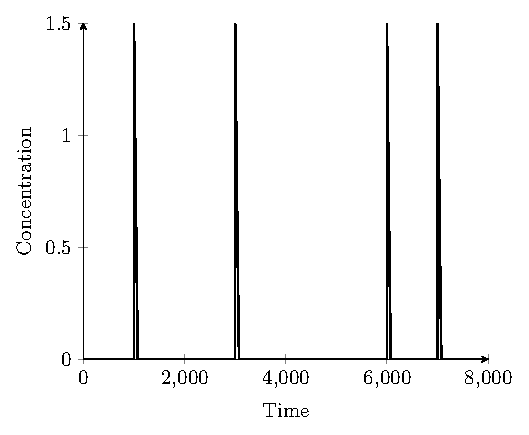
\includegraphics[width=9cm]{or_input}
		\caption{Input Stream}
		\label{fig:ORinput}
		\vspace{15mm}
	\end{subfigure}
	\\
	\begin{subfigure}[b]{0.9\textwidth}
	    \centering
		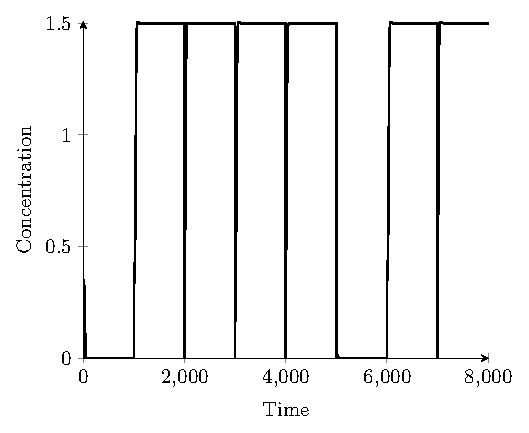
\includegraphics[width=9cm]{or_output}
		\caption{Output Stream}
		\label{fig:OROutput}
	\end{subfigure}
	\caption[Concentration Traces for Perceptron/Delay Line Learning Logic OR]{Example concentration traces of binary time series chemical perceptron that successfully learns OR function. Left shows input stream 0,1,0,1,0,0,1,1. Right shows correct output stream of 0,1,1,1,1,0,1,1. Two zeros on the input stream at 4,000 and 5,000 successfully produce zero at time 5,000 on output stream.}
	\label{fig:ORPerceptResults}
\end{figure}

NAND, IMPL, and NOTX1 are all heavily dependent on the last input to resolve in the time delay line, $X1$. The input species $X1$ is not provided to the system until typically 50 time steps later than value $X2$. The original model of the perceptron was optimized for instantaneous and simultaneous injection of both inputs. Because input $X1$ is not ready, the performance is lower because that input plays a larger role on the correct performance for these logic functions. This makes the system capable of obtaining an average success rate of approximately 90\% compared to the perceptron's 99\% success rate~\cite{Banda2014-bp}.

\section{Deoxyribozyme Cascading Implementation}
\label{sec:deoxy}
Now, we would like to present how such a delay line could be realized in a system employing deoxyribozyme catalysis~\cite{Stojanovic2003-eg}~\cite{Stojanovic2000-qx}~\cite{Liu2009-jz}. Figure~\ref{fig:deoxy1} shows an example of a two stage manual delay line with the signals being the deoxyribozymes $X1_{signal}$ and $X2_{signal}$ which cleave the substrate $X$ at the embedded ribonucleotide. This produces $X1$ ready for the next system to consume. Subsequently, $X1C$ embedded with another ribonucleotide is able to get cleaved by deoxyribozyme $X2_{signal}$ to form the next input to the system, $X2$.

\begin{figure}[ht]
	\centering
	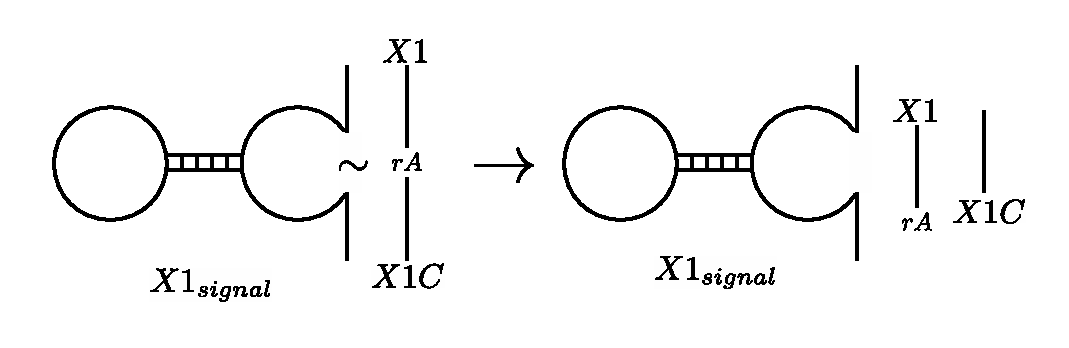
\includegraphics[width=12cm]{cleavage}
	\caption[Example of Deoxyribozyme Implementation]{Deoxyribozyme cascading example. Deoxyribozyme $X1_{signal}$ cleaves $X$ at embedded ribonucleotide ($rA$) to form $X1$ and $X1C$. A similar process occurs on $X1C$ to produce $X2$ and $X2C$.}
	\label{fig:deoxy1}
\end{figure}

\section{Discussion}
We have presented a novel implementation of a delay line as a chemical reaction network capable of storing past concentrations. By arranging our delay lines in a SIMD-like layout, we could delay multiple segments of data simultaneously with a shared control signal for either model of delay line. We have introduced two types of a chemical delay line: manual copy delay line and backwards propagation delay line. A manual copy delay line can precisely carry values in a delayed state, but requires more intervention from the user (growing at a rate of $m$) to propagate values through the system. The second model, backwards propagating delay line, automatically moves values through the system with a single signaling injection with reasonable accuracy.

The integration of the backwards propagating delay line with the threshold asymmetric signal perceptron resulted in the first chemical model capable of learning binary time series. Also, this example is a proof-of-concept that our delay line is a modular block ready for use in other systems. For systems requiring a smaller window of past values, either model of the delay line gives sufficient accuracy for data storage. The manual copy delay line shows potential for longer chains with the amount of calculated SAMP passed between phases remaining below 0.01\% for a delay line of 10 stages. The backwards propagating delay line provides a much simpler user interface at the sacrifice of accuracy. A backwards propagation of five stages keeps the calculated SAMP below 15\%. Systems requiring a large number of delays will have to weigh accuracy and simplicity to make a selection for a particular implementation.

The \gls{bpl} and \gls{mdl} tied with a \gls{asp} demonstrate how these two systems can modularly connect to other elements in a \gls{crn} to form a memory. Now that there are the building blocks to provide data storage in a \gls{crn}, we discuss the work to find the optimal size of memory and layout of \gls{ann} to solve the ant trail task when paired with a delay line.




\glsresetall
\chapter{Trail Runner and Trail Viewer}
\label{chap:trail_runner}
This chapter discusses the pair of tools developed for simulation and analysis of the John Muir, Santa Fe, and other trails prior to moving to a \gls{crn} environment. We found no other application that readily performed the evaluation required for our work so we developed two applications to aid in our research. The two applications, trail runner and trail viewer, are built on published, open-source tools and were designed with extensibility in mind.  Trail runner is a parallel \gls{ga} trail evaluator that manipulates parameters of the simulations and records the runs to a database. Trail viewer is a web-based application that allows users to filter, browse, and view the results from various types of trail simulations. This framework allowed us to easily sweep across different parameters to locate an ideal configuration for later implementation in a \gls{crn}. In this chapter, we will discuss both tools, some of the advantages of these tools, and their framework.

\section{Trail Runner}
Trail runner is responsible for evaluation of different networks to see performance against navigating the agent through different trails (like the John Muir, Santa Fe, and more). Trail runner also performed evolution of the parameters on the networks with \glspl{ga} working towards the maximum performance possible. We have also published trail runner under an open source license and it is available for download at \url{https://github.com/jmoles/trail-runner}. The application is a command line-based Python tool that uses published tools for evaluation of the \glspl{ann} through evolutions in a \gls{ga}.

The \glspl{ann} in trail runner were modeled with PyBrain, a machine learning library for Python~\cite{Schaul2010-tu}. PyBrain served as the basic model for the different flavors of \glspl{ann}. The evolution of the parameters on the \glspl{ann} is performed with \gls{deap}~\cite{Fortin2012-yv}. \gls{deap} is a powerful toolbox allowing straightfoward evaluation of \gls{ga} in Python. One of the primary reasons for the selection of \gls{deap} was the tightly integrated use of a distributed computing framework, \gls{scoop}~\cite{Hold-Geoffroy2014-qf}. \gls{scoop} allowed the distributing of work across multiple servers in the lab cluster for reduced run time. With the use of PyBrain, \gls{deap}, and \gls{scoop}, we then had to build a series of tools to evaluate the different trails and report the results.

The intent of trail runner is to allow evaluation of different \gls{ga} and \gls{ann} parameters to attempt and find an ideal solution prior to implementation in a \gls{crn}. Evaluating the same \gls{ann} in a \gls{crn} (with a tool like \gls{coel}~\cite{Banda2014-qw}) can take a substantially longer amount of time. Performing the same optimization in a \gls{crn} from the beginning would have caused the amount of time to simulate this project to increase dramatically. Later, we will show some examples of the speedup with \gls{scoop} and running the same network in \gls{coel}. Easily sweeping across different parameters in trail runner allowed us to narrow the set of potential parameters to run simulations against.

Running the trail runner application is relatively straightforward after users have configured a database for the application to record results and retrieve available configuration parameters. Trail runner uses PostgreSQL~\cite{The_PostgreSQL_Global_Development_Group1996-qt} and includes a script to create the initial database and populate it with the networks and trails used in this work. A safe set of defaults are specified for many of the \gls{ga} parameters, but they are all customizable by the user using command line flags. A few of the key parameters as an example include the trail ID, population size, maximum moves, network ID, and generations to run for. A full list of the available parameters are available in the application's help (\texttt{--help}).

Trail runner took advantage of these tools for evaluation of the trail task. Testing on the tools was performed by first starting with a smaller trail shown in Figure~\ref{fig:test_trails}. Afterwards, we moved on by testing the larger John Muir trail and got results similar to that of Jefferson's. Section~\ref{sec:tools_testing_results} discusses the results of testing against test trail 1, test trail 2, and the John Muir trail.

\begin{figure}
\centering
\begin{subfigure}[b]{.5\textwidth}
    \centering
    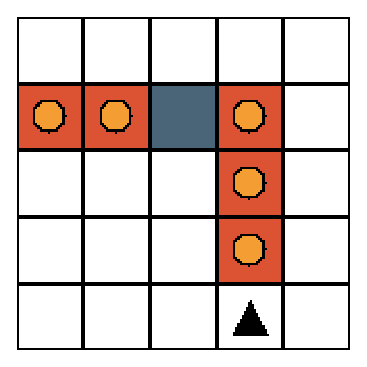
\includegraphics[width=.4\linewidth]{small_trail_1}
    \caption{Test trail 1}
    \label{fig:test_trail_1}
\end{subfigure}%
\begin{subfigure}[b]{.5\textwidth}
    \centering
    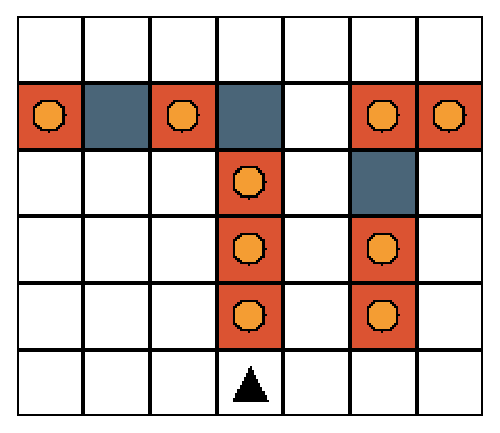
\includegraphics[width=.5\linewidth]{small_trail_2}
    \caption{Test trail 2}
    \label{fig:test_trail_2}
\end{subfigure}
\caption[Two Test Trails]{The two trails used for initial testing of trail runner. They are designed for fast evaluation as well as a small complication (turns, gaps) so that some \gls{ga} optimization is necessary. Test trail 1 is simpler than the test trail 2 on the right.}
\label{fig:test_trails}
\end{figure}

\section{Trail Viewer}
Trail viewer is a Flask~\cite{Ronacher2010-mn} web-based application that allows viewing of results from trail runs over their \gls{ga} evaluation. Diagrams of results are rendered with the help of matplotlib~\cite{Hunter2007-yc} and Plotly~\cite{Plotly2012-po}. The trail diagrams (like the ones in Figure~\ref{fig:test_trails}) used throughout this paper are also rendered using trail viewer. At the time of this writing, an instance of trail viewer is operating at \url{http://codeboxide.joshmoles.com}. Figure~\ref{fig:trail_viewer_ss} shows a screen shot of the trail viewer application. Trail viewer is also available under an open source license for download at \url{https://github.com/jmoles/trail-viewer}.

Early versions of trail viewer were a desktop-based \gls{gui}. The application was migrated to a web-based tool for greater compatibility with different operating systems as well as allowing interaction with other web-based tools (like \gls{coel}~\cite{Banda2014-qw} and Plotly~\cite{Plotly2012-po}). Trail viewer also interacts with the same database that trail runner writes results from each run. Trail viewer only consumes information from the database and does not perform any modification. Animation of the agent navigating through the trail is also available in trail viewer. Trail viewer uses JavaScript to render the agent navigating through the trail with a specified trail and moves. The diagrams showing the moves the agent traveled (for example, Figure~\ref{fig:trail1_final_gen}) were captured with the help of this capability.

\begin{figure}
\centering
\includegraphics[width=13cm]{trail_viewer_ss}
\caption[Screen Shot of Trail Viewer]{Screen shot of the trail viewer application showing the results of a single simulation run. The information of the trail and simulation configuration is shown at the top with the partial charts of results shown below.}
\label{fig:trail_viewer_ss}
\end{figure}

The pair of these applications provide an environment to evaluate different types of networks and trail problems with numerous sets of parameters and view the results. The integration of PyBrain, \gls{deap}, and \gls{scoop} create a platform that allows others to easily run research similar to that of Jefferson or Koza on the John Muir, Santa Fe, or other trail of choosing. Users can easily add their own databases, networks, or \gls{ga} parameters and generate plots showing a single configuration run, an average of all runs with these parameters, or evaluate a sweep of different parameters, such as delay line length.

In the next chapter, we present the use of trail runner and trail viewer to arrive at the minimal delay line length for implemenation in a \gls{crn}.

\glsresetall
\chapter{Non-Chemical Reaction Network Simulations}
\label{chap:non_crn_testing}
This chapter looks at the testing performed using trail runner and trail viewer in a non-\gls{crn}. We will go over a set of test cases that were first preformed to validate that trail runner and trail viewer were presenting accurate results. The next set of tests will move toward identifying the minimal length of delay line necessary to evaluate the trail for later implementation as a \gls{crn}. We first cover the methodology we used for the testing and present the results. The chapter concludes with a discussion of the results.

\section{Methodology}
\label{sec:trail_runner_methods}
In this section, we will outline how we verified that trail runner functioned as expected and later used to find the optimal length of delay line. We did the evaluation testing on three trails: test trail 1, test trail 2 (Figure~\ref{fig:test_trails}), and the John Muir Trail (Figure~\ref{fig:johnmuirtrailimage}). We developed a genetic algorithm based off a simple straightforward algorithm proposed by B\"{a}ck~\cite{Baeck2000-co}. A version of this algorithm was already implemented in \gls{deap}, known as \texttt{varAnd}~\cite{Fortin2012-yv}; however, the algorithm did not have all of our desired functionality. Namely, we wanted the ability to monitor the progress of the \gls{ga} in real time, so we used it as a basis for our \gls{ga}. It also did not directly support the selection method we used, $(\mu + \lambda)$ selection~\cite{Schwefel1976-er}. Figure~\ref{fig:ga_flowchart} shows a flowchart of this process discussed that you may find helpful while reading this section.

\begin{figure}[p]
\centering
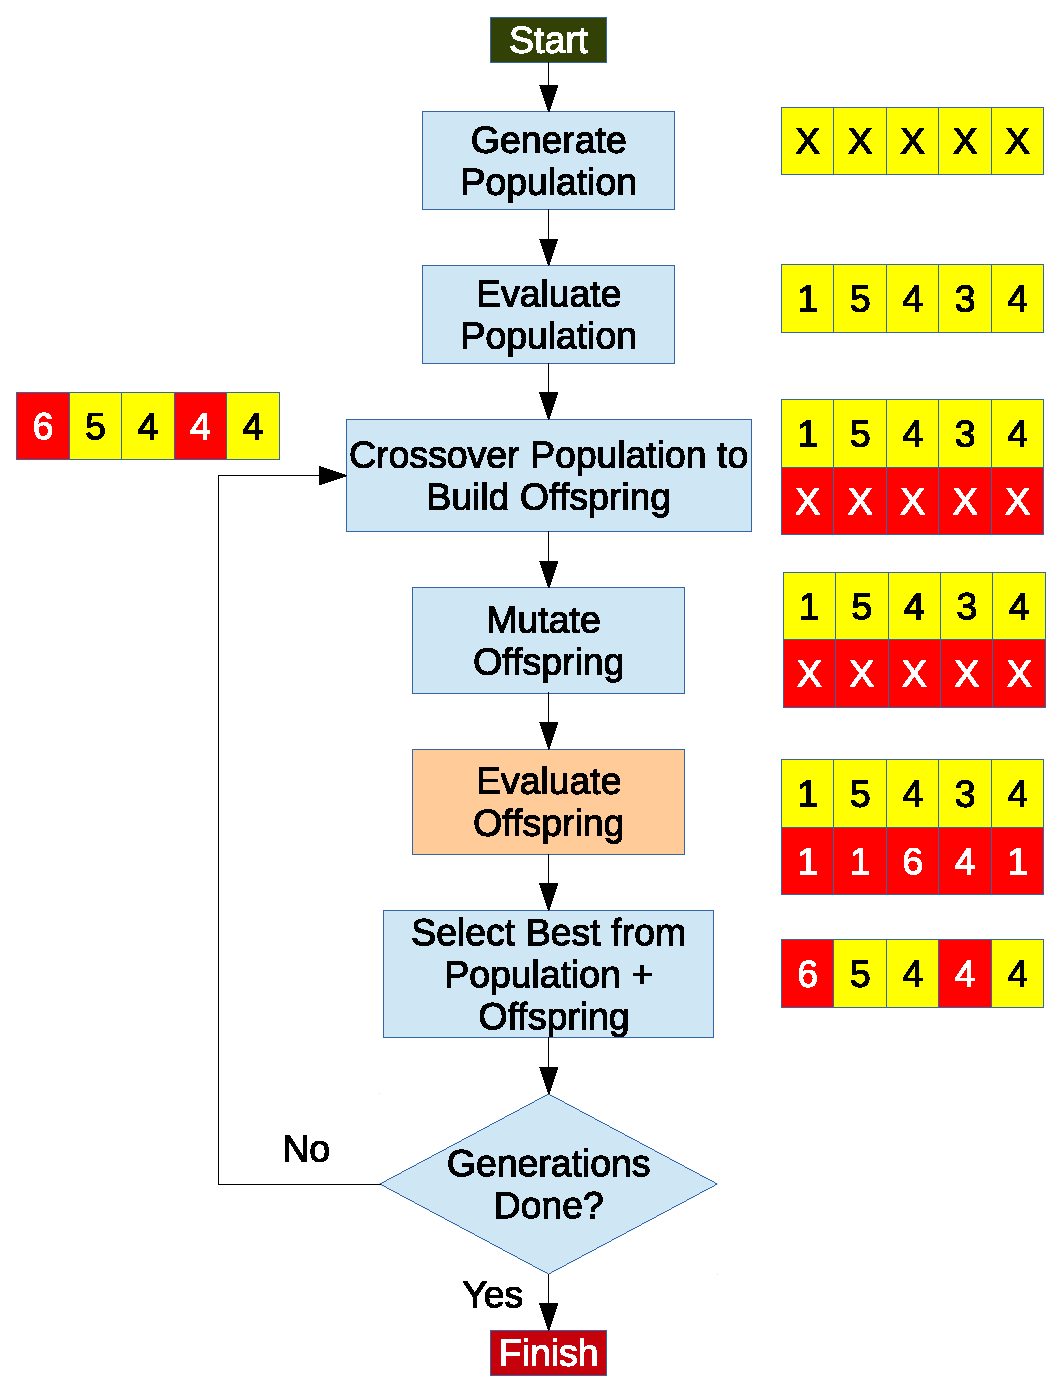
\includegraphics[width=.8\textwidth]{ga_flowchart}
\caption[Genetic Algorithm Flow Chart]{Flowchart of the \gls{ga} used to test the trails. Based off the algorithm proposed by \cite{Baeck2000-co} and \cite{Fortin2012-yv}. The boxes to the right and left each represent an individual through each phase of the \gls{ga}. An $X$ indicates the fitness is unknown and a number represents a fitness (higher is better). The pool to the left of crossover population represents the indivuals selected and looping back on the ``No'' path from ``Generations Done''.}
\label{fig:ga_flowchart}
\end{figure}

The \gls{ga} we used started by generating a population with a size, $P$, defined by the user. The individuals in this pool are a set of real-valued vectors that are in the period between the minimum weight and maximum weight, or $[w_{min}, w_{max}]$. Each of these values corresponded to a weight connecting perceptrons on the \gls{ann}. Each individual is then evaluated to determine their fitness by running them for $M$ moves through the specified trail. The intent was to find all pieces of food before focusing on minimizing the number of foods. We wanted to place greater emphasis on the amount of food consumed, so fitness ($f$) is calculated by:

\begin{equation} \label{eq:fitness_equation}
f = 1.0 \times food\:consumed - 0.1 \times moves\:taken
\end{equation}

Afterwards, we crossover the population with a two-point crossover~\cite{De_Jong1975-wc} with a specified probability of undergoing crossover, $p_x$. If an individual does not get selected for crossover, it is copied to the pool of offspring.

Next, a Gaussian mutation method is used on the pool of offspring because of it's common use for real-valued vectors~\cite{Baeck2000-co}. All individuals enter mutation in this algorithm and each real value of the chromosome is adjusted with a probability of mutation, $p_m$. Then, these offspring are evaluated and assigned their fitnesses before entering selection. Our selection selected the best $P$ individuals from the pool of offspring and the original population. This selection method is also known as $(\mu + \lambda)$~\cite{Schwefel1976-er}. We then continue to repeat this process until one of the three criteria for exiting are met:

\begin{itemize}
\item the user specified number of generations ($G$) are evaluated,
\item all food in the trail is consumed, or
\item or there has been no change in the standard deviation of the mean fitness ($m_g$) of the individual pool for the previous $g$ generations.
\end{itemize}

The final termination criteria was added to save processing time for this task. We found that if the average was stuck at this point for a long period of time. The likelihood of one of these runs with the stuck average proceeding to increase fitness was low. Also, the amount of time in general to solve this problem was rather large so terminating an evaluation that is not progressing is more advantageous than waiting. Note that by terminating when all food is consumed means no optimization for the number of moves taken. The goal was to consume all of the food in the provided number of moves. We will show an example in the results where we terminated a run early with no change in mean fitness.

The algorithm itself had several parameters, such as population, probabilities, and generations, that we must specify. Values were selected based of recent publications as a starting point for evaluation of the \gls{ga}. We selected a population, $P$, of 100 with a probability of crossover, $p_x$, of 0.6 based off work by De Jong et. al.~\cite{De_Jong1991-cq}. For the test trails, we selected a smaller population of 10 to reduce the probability of a solution at generation 1. In other words, we wanted to force the \gls{ga} to operate rather than potentially randomly finding a good candidate on the first run for such a small trail. We selected a probability of mutation, $p_m$, of 0.05 from De Jong's thesis work~\cite{De_Jong1975-wc}. Weights in the range of $[-5.0, 5.0]$ were selected for the neural networks. We set the number of generations ($G$) to a relatively high value of 5000 generations because we generally found that either all food was consumed or the value of $m_g$ settled and exited early prior to reaching 5000 generations. A summary of these parameters is shown in Table~\ref{tab:testing_run_parameters}.

\begin{table}[ht]
\centering
\begin{tabular}{ll}
\textbf{Parameter}                  & \textbf{Value} \\ \hline
Population ($P$)                    & 100 (10 for Test Trail)   \\
Probability of Mutation ($p_m$)     & 0.05  \\
Probability of Crossover ($p_x$)    & 0.6  \\
Generations ($G$)                   & 5000  \\
Mean Fitness Generations ($g$)      & 300  \\
Weight Range ($[w_{min}, w_{max}]$) & $[-5.0, 5.0]$
\end{tabular}
\caption[Summary of GA Parameters for Test Runs]{This table summarizes the parameters used for the test runs in this chapter. The population and probabilities are based of work by De Jong in \cite{De_Jong1991-cq} and \cite{De_Jong1975-wc}. The generations, mean fitness generations, and weight range are set to allow ample exploration.}
\label{tab:testing_run_parameters}
\end{table}

Using this \gls{ga} configuration, we tested the \gls{ga} against test trail 1, test trail 2, John Muir trail, and performance evaluations on the Santa Fe trail. For each trail, we limited the number of moves to 10, 20, 100, and 200, respectively. The test trail values is based off the minimum number of moves necessary plus a small overhead. The values for the John Muir and Santa Fe trail are the same used by Jefferson~\cite{Jefferson1992-ph} and Koza~\cite{Koza1992-xs}. These values are summarized in Table~\ref{tab:testing_moves_limit}. For this verification exercise, we use a neural network that is the same layout as the one Jefferson used to original solve the John Muir trail. 

\begin{table}[ht]
\centering
\begin{tabular}{lcccc}
\textbf{Trail}  & $\bm{M}$  & \textbf{Min. Moves} & \textbf{Food} & \textbf{Max. Fitness} \\ \hline
Test 1    & 10  & 7   & 5  & 4.3 \\ 
Test 2    & 20  & 14  & 9  & 7.6 \\
John Muir & 200 & 147 & 89 & 74.3 \\
Santa Fe  & 400 & 165 & 89 & 72.5
\end{tabular}
\caption[Moves Limits for Test Runs]{We show the statistics for the trails used in this chapter. The move limits ($M$) for test trails are slightly more than the minimum number of moves for each and the John Muir and Santa Fe the same values as Jefferson and Koza. The maximum fitness is calculated with Equation~\ref{eq:fitness_equation}.}
\label{tab:testing_moves_limit}
\end{table}

Next, we were looking to find the minimal length of delay line connected to the smallest \gls{ann} for consuming the most amount of food in the trail. To reduce the time required for each evolution, we started evaluation on three trails that are a subset of the Santa Fe trail~\cite{Koza1992-xs} as well as testing on the full trail. The Santa Fe trail was selected as the main evaluation trail in a chemistry because Koza claimed it is a more difficult trial. It is also a more common trail in literature today for testing. Figure~\ref{fig:sft_segments} show segments 1, 2, and 3 of the Santa Fe trail. They were extracted as the first portions of the full Santa Fe trail that the agent would normally navigate through.

\begin{figure}
\centering
\begin{subfigure}[b]{.5\textwidth}
    \centering
    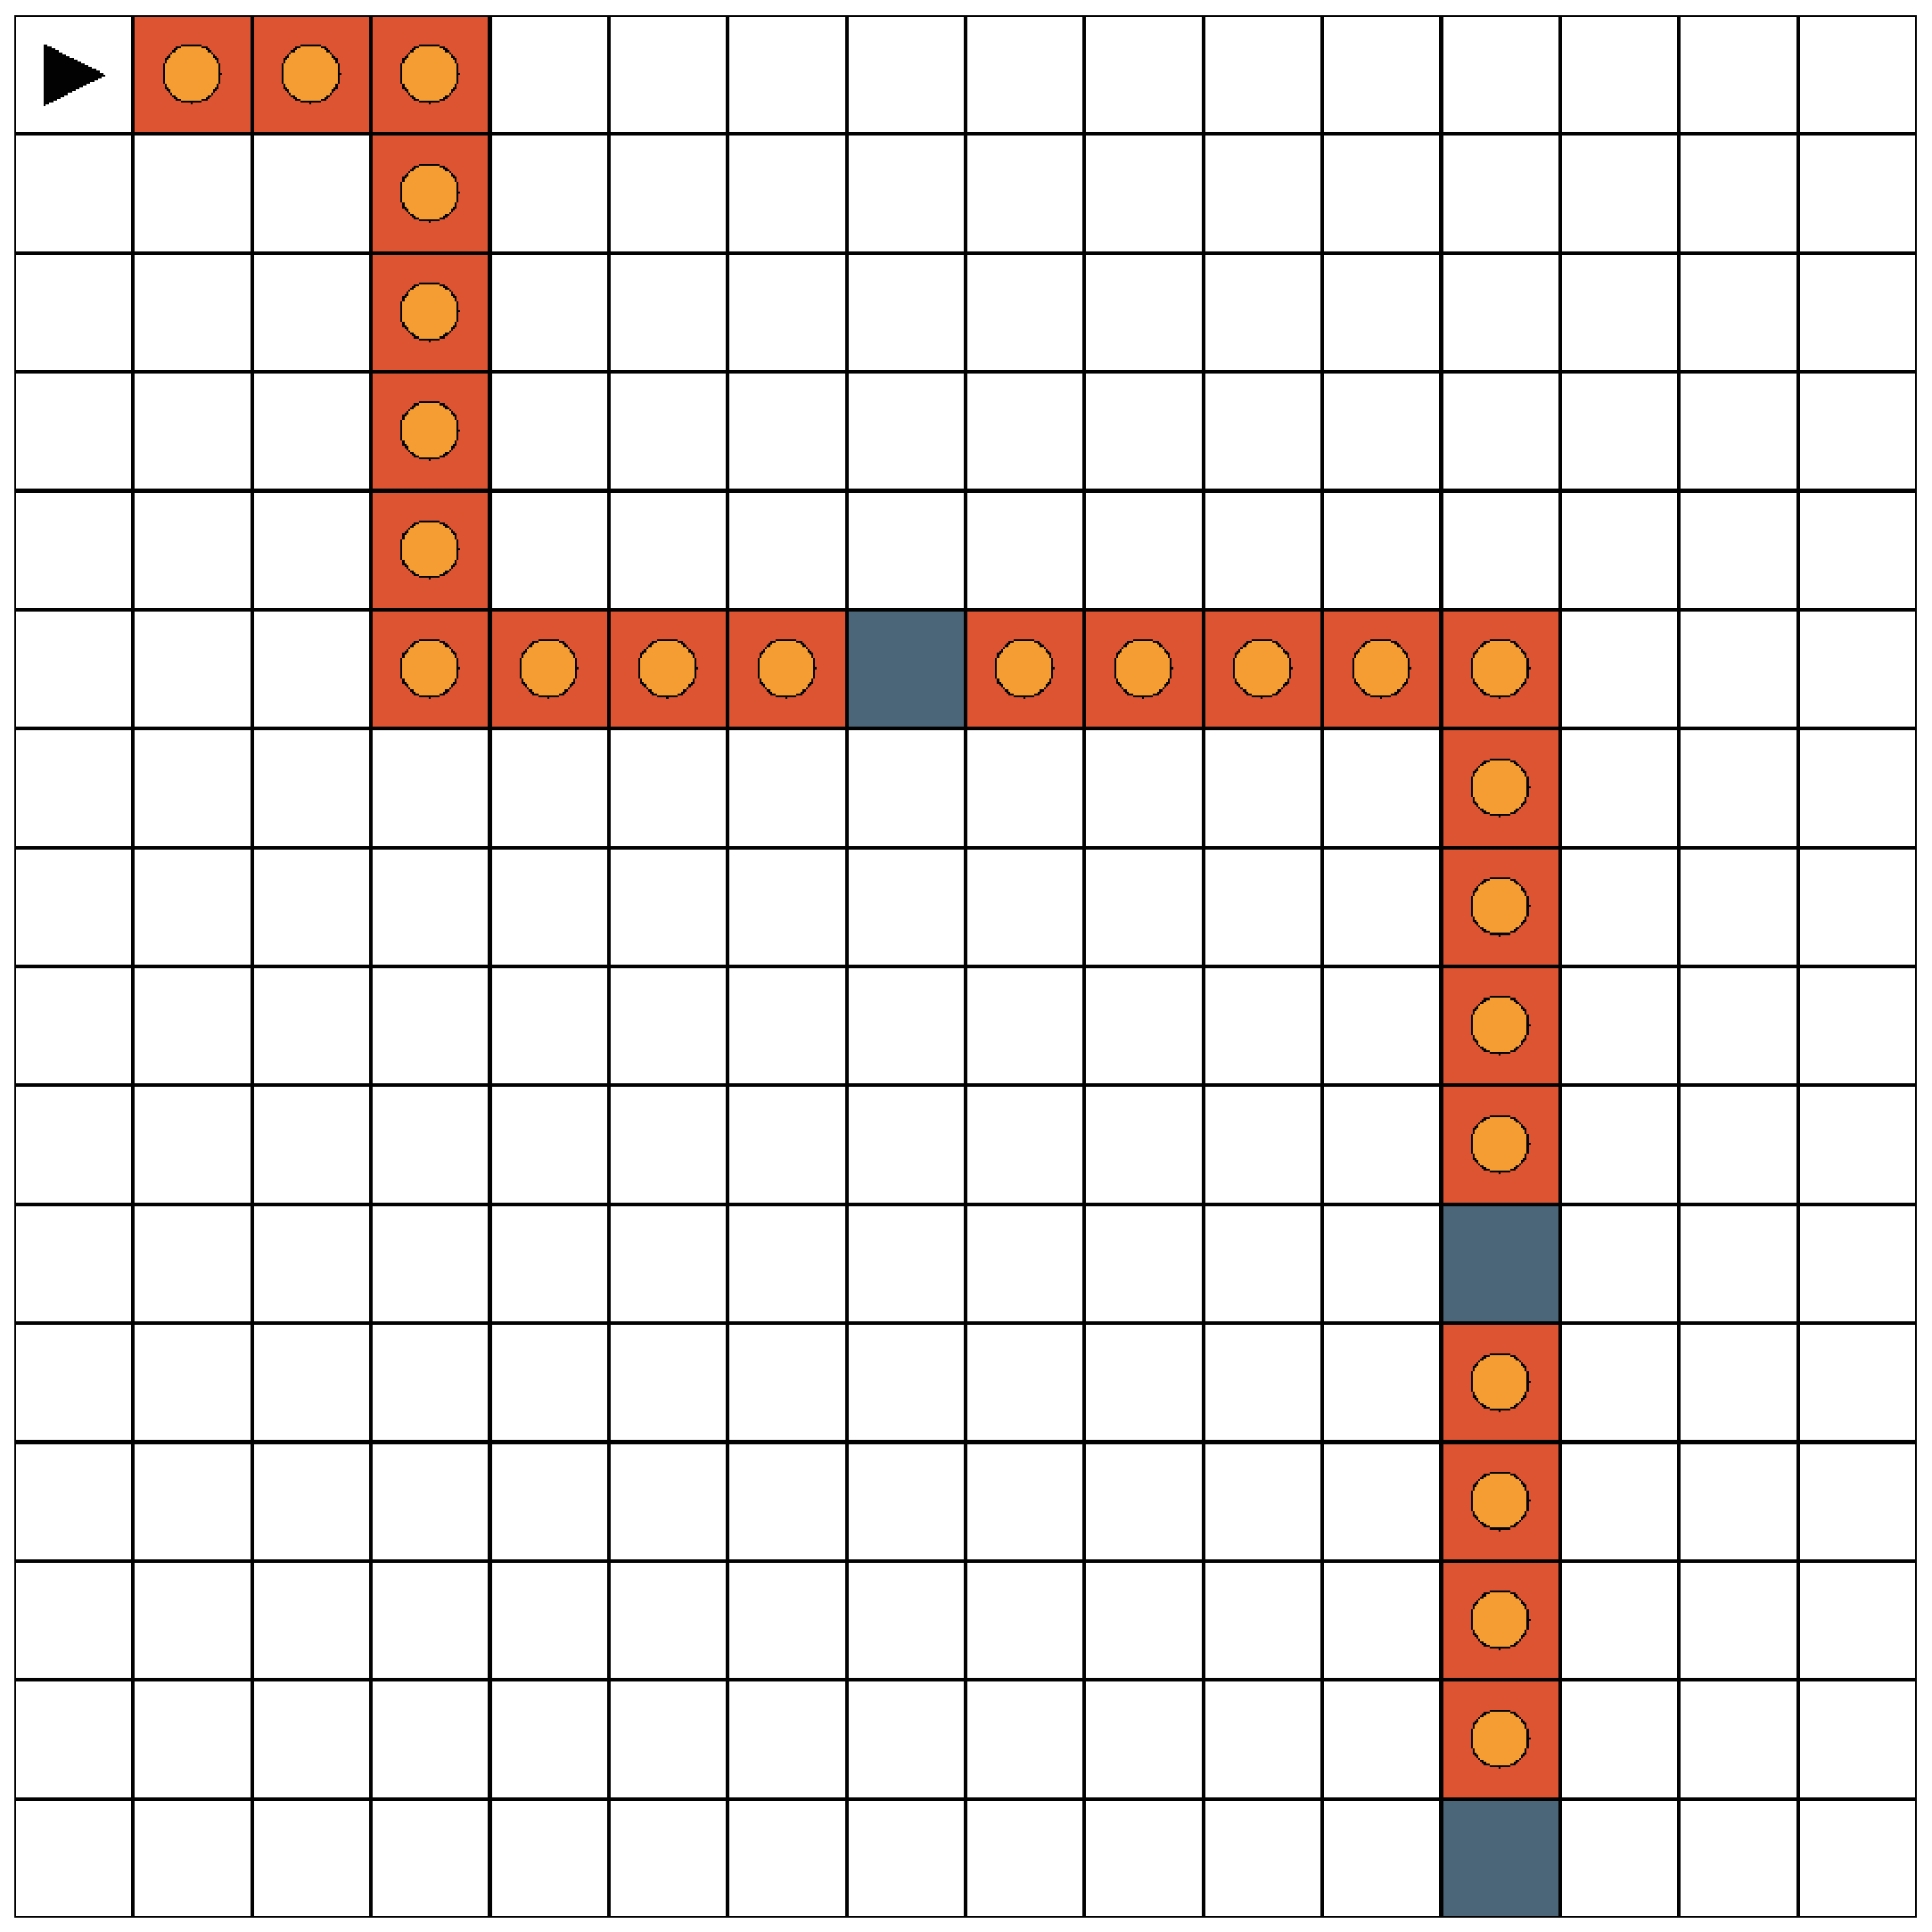
\includegraphics[width=0.5\linewidth]{santa_fe_seg1_17}
    \caption{Santa Fe Trail Segment 1 (Easy)}
    \label{fig:sft_seg1}
\end{subfigure}%
\begin{subfigure}[b]{.5\textwidth}
    \centering
    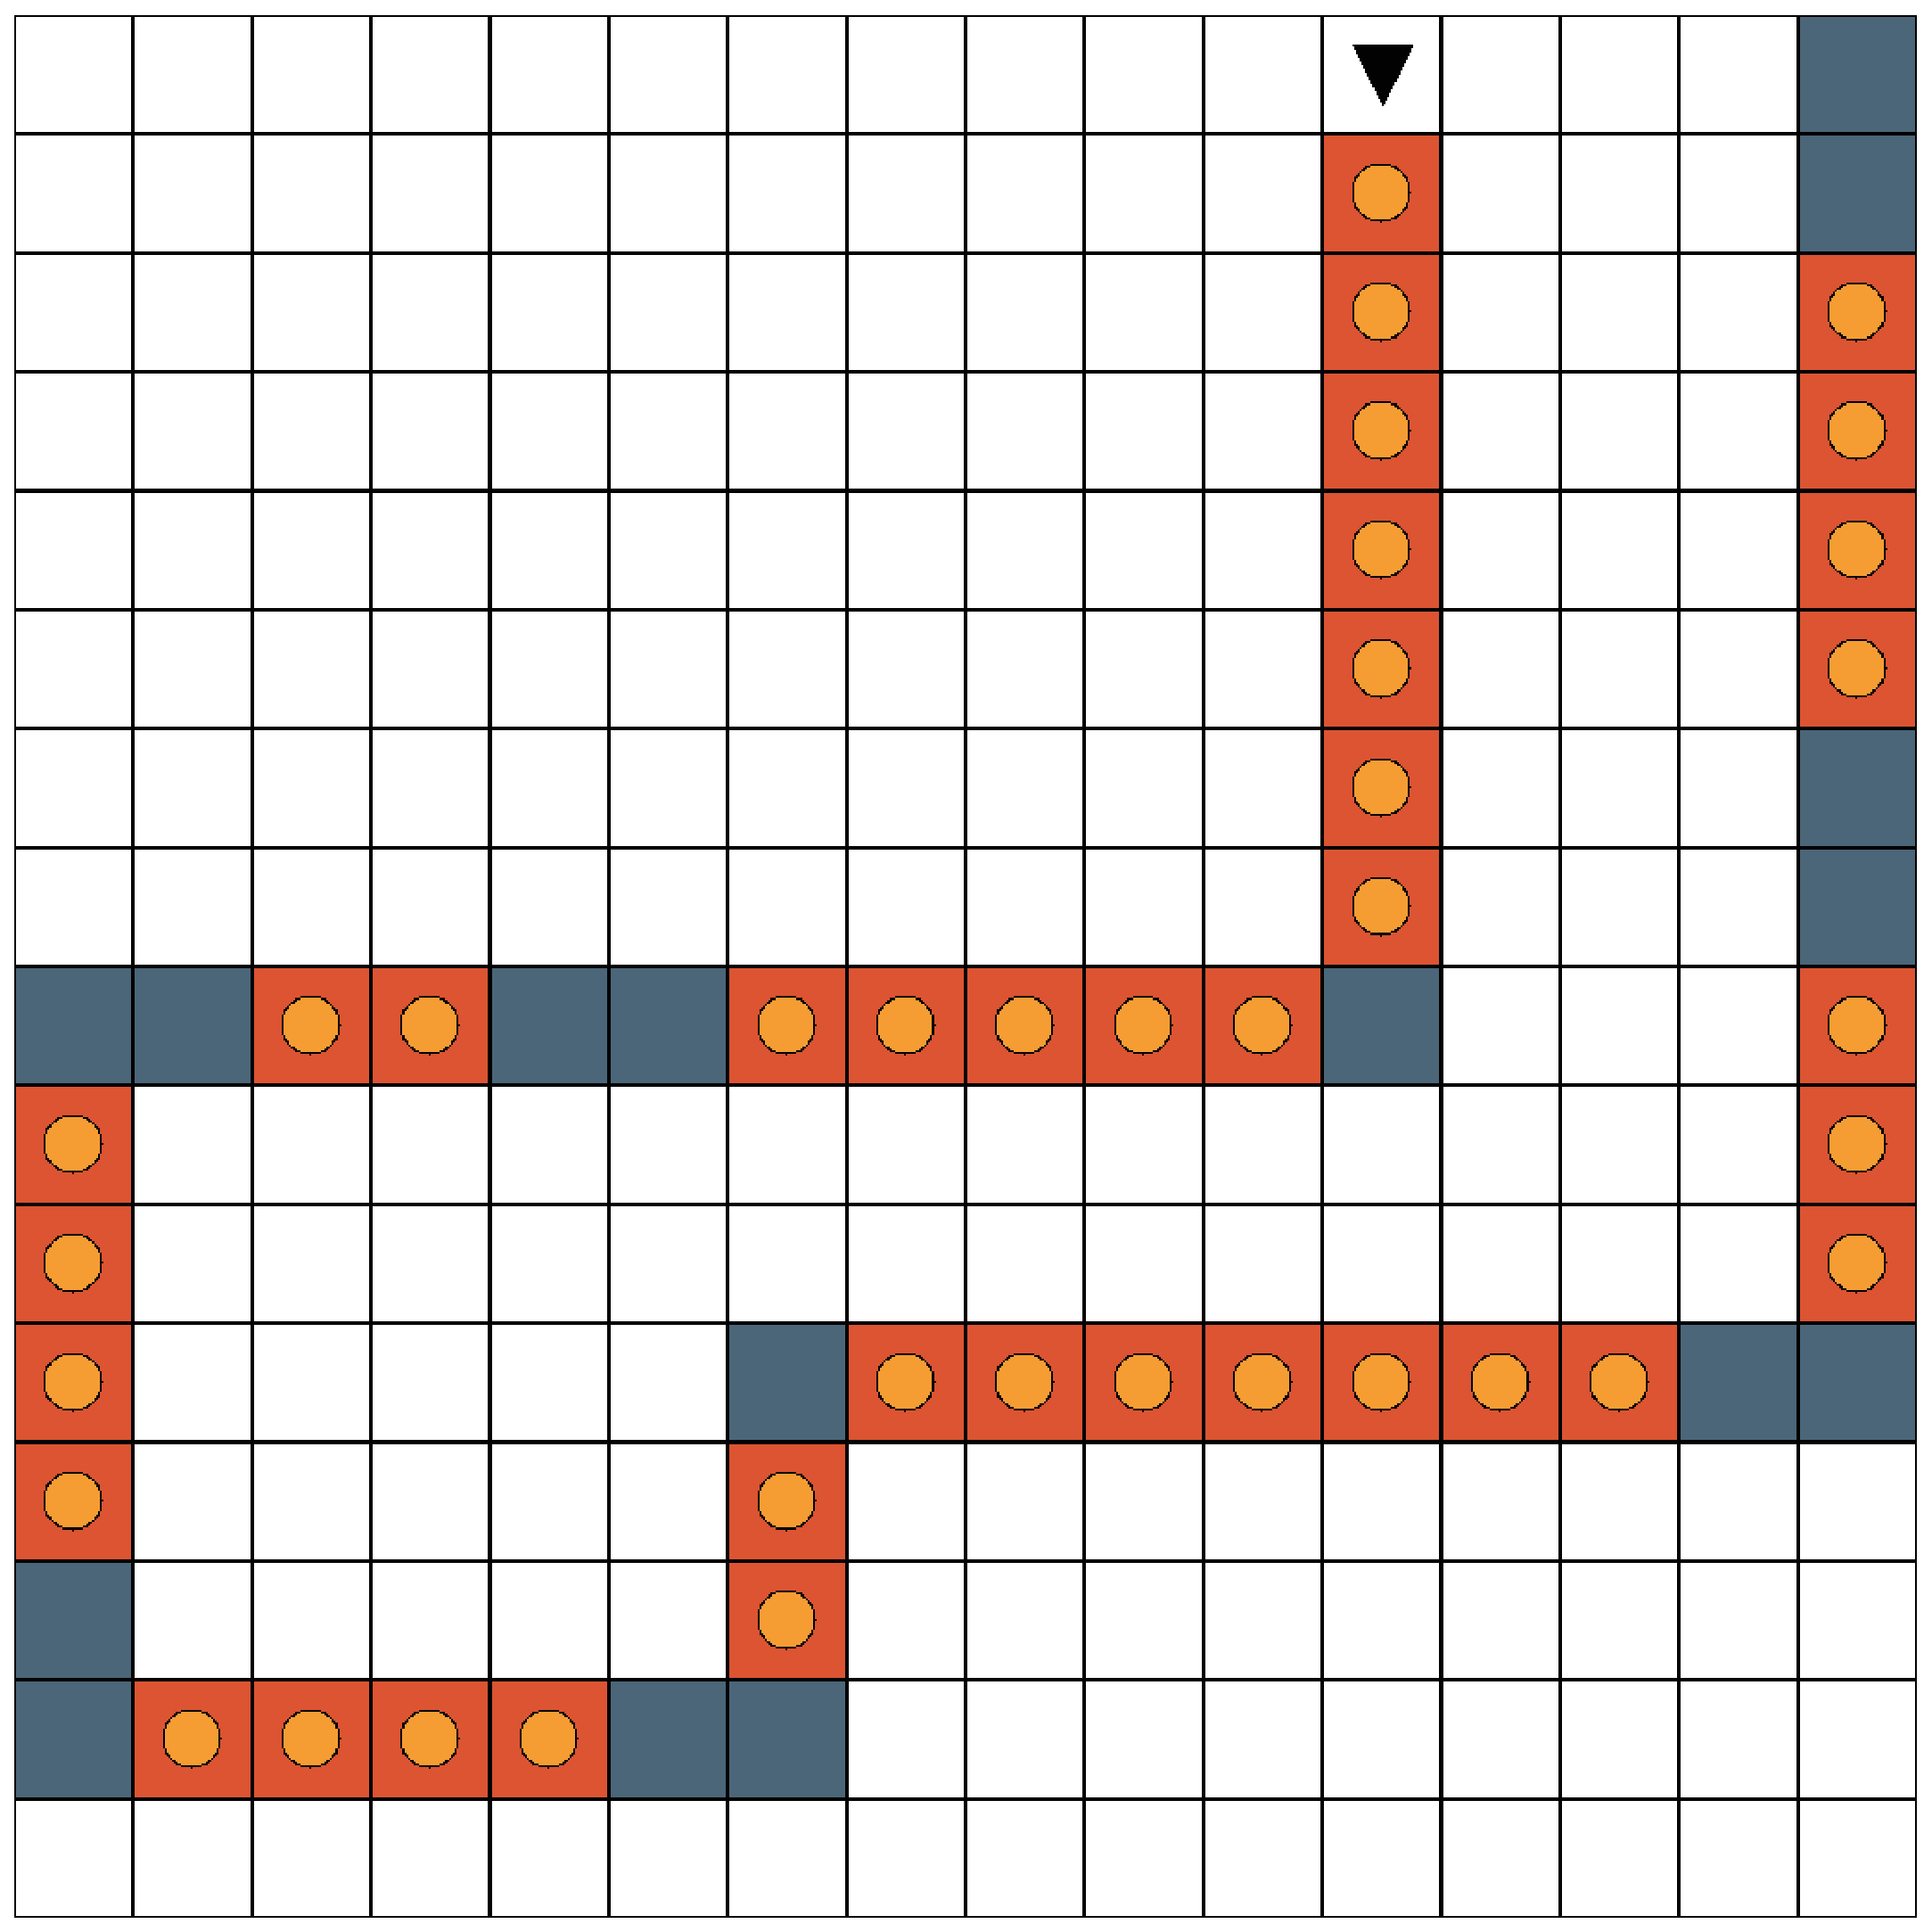
\includegraphics[width=0.5\linewidth]{santa_fe_seg3_19}
    \caption{Santa Fe Trail Segment 3 (Medium)}
    \label{fig:sft_seg3}
\end{subfigure}
\\
\begin{subfigure}[b]{0.5\textwidth}
    \centering
    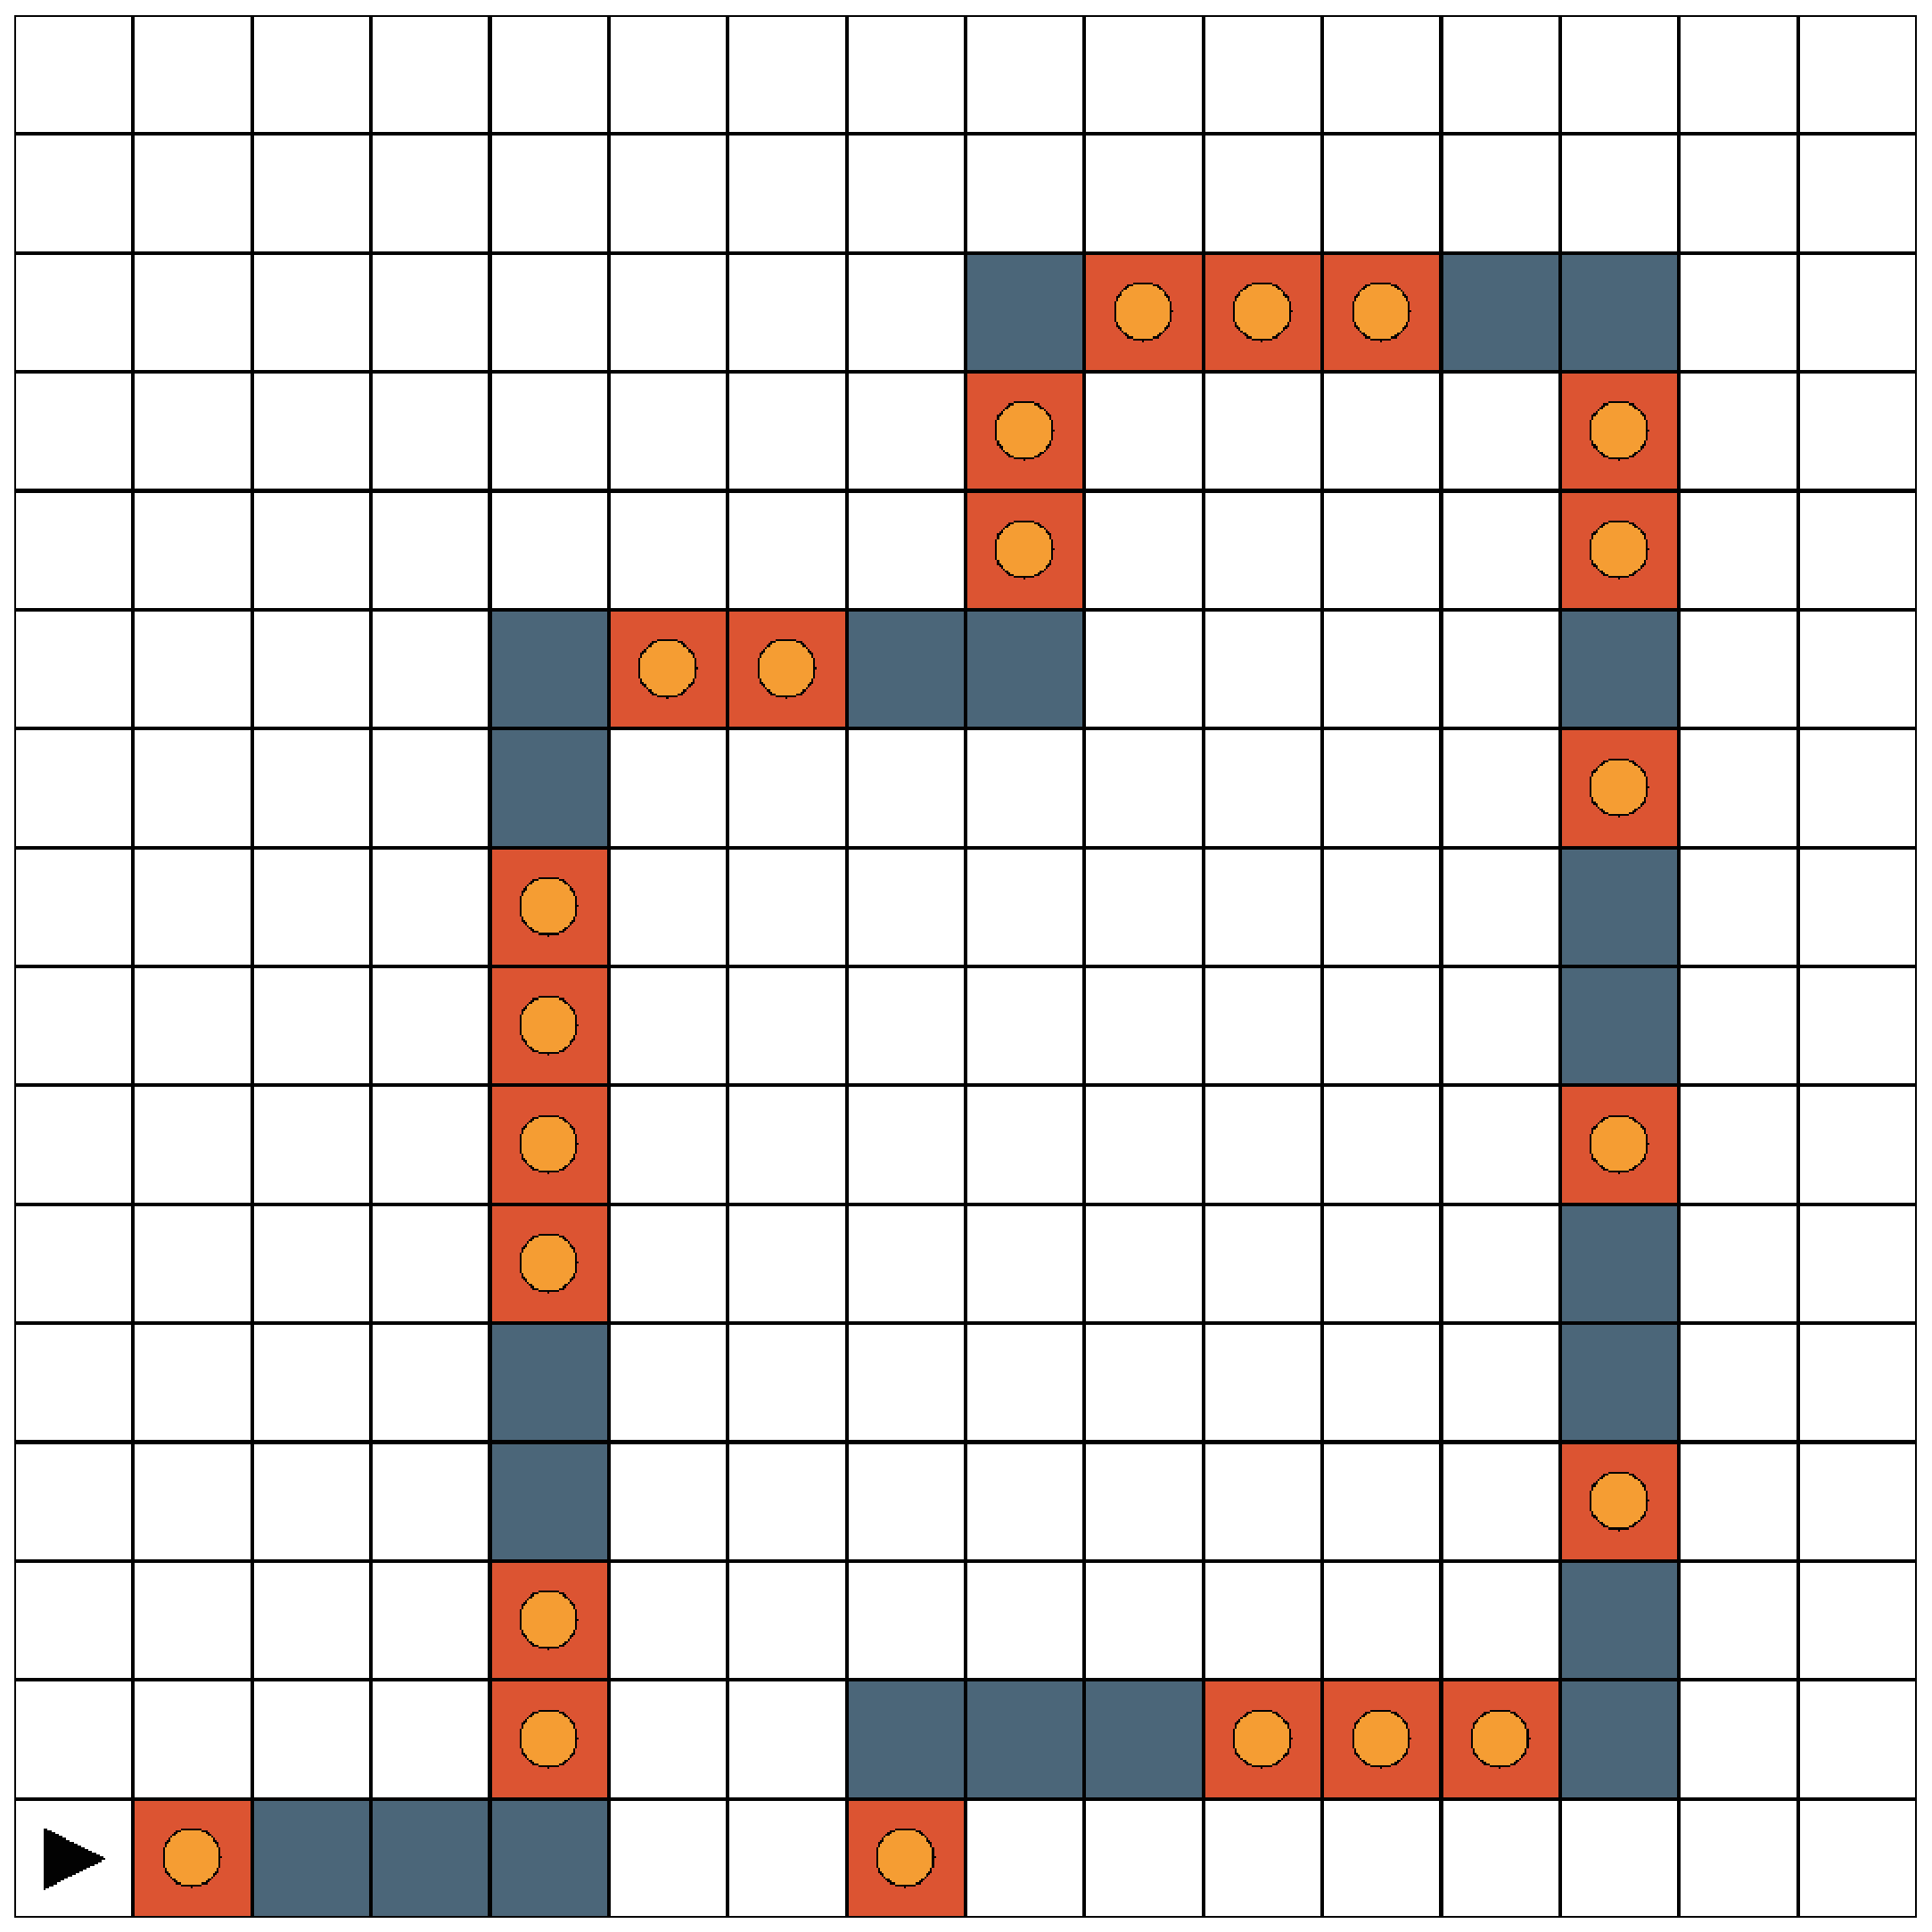
\includegraphics[width=0.5\linewidth]{santa_fe_seg2_18}
    \caption{Santa Fe Trail Segment 2 (Hard)}
    \label{fig:sft_seg2}
\end{subfigure}
\caption[Three Santa Fe Trail Segments]{The three trails with increasing difficult that were used for the delay line length optimization. The number of gaps and turns increases with each trail is the determination for the difficulty.}
\label{fig:sft_segments}
\end{figure}

We used the same \gls{ga} configuration as mentioned above. The moves limit was divided by four ($M = 400 / 4 = 100$) since each trail segment represents a 16 x 16 area which is a quarter of the full Santa Fe trail. Keeping all other parameters the same, we then started going across delay line lengths of $N=2$ all the way up to $N=16$ to search for the minimal length of delay line. 

Like Jefferson's neural network, we had to have a ``food ahead'' and ``not food ahead'' to activate the \gls{ann} in the case of no food ahead. Every delay line segment required two input nodes to hold values. An example \gls{ann} with a delay line of length two is shown in Figure~\ref{fig:trail_ann_w_dl2}. There are a couple of changes from the neural network originally used by Jefferson (see Figure~\ref{fig:jefferson_original_nn}). Our experiments found that only one hidden node in the \gls{ann} was sufficient to solve the task when paired with a delay line. Like Jefferson and Koza, we also found that the ``None'' (meaning no move) output from the \gls{ann} was not used by the best individuals~\cite{Jefferson1992-ph}~\cite{Koza1992-xs}. So, the number of total nodes in the system is represented by Equation~\ref{eq:node_count_eq}.

\begin{equation} \label{eq:node_count_eq}
n = 2 \times delay\:line\:length + 4
\end{equation}

\begin{figure}
\centering
\begin{tikzpicture}[->,draw=black!100, node distance=\layerseptikznn]
    % Based off code form http://www.texample.net/tikz/examples/neural-network/
    \tikzstyle{every pin edge}=[<-,shorten <=1pt]
    \tikzstyle{neuron}=[circle,draw=black!50,fill=white!25,minimum size=25pt,inner sep=0pt]
    \tikzstyle{input neuron}=[neuron, draw=black!50, fill=Accent-5-1];
    \tikzstyle{output neuron}=[neuron, draw=black!50, fill=Accent-5-3];
    \tikzstyle{blank neuron}=[neuron, draw=white!50, fill=white!50];
    \tikzstyle{hidden neuron}=[neuron, draw=black!50, fill=Accent-5-2];
    \tikzstyle{annot} = [text width=4em, text centered]
    \tikzstyle{dlbox}=[rectangle,draw=black!50,fill=Accent-5-4];
    \tikzstyle{input value}=[circle,draw=black!50,fill=Accent-5-5!50,minimum size=25pt,inner sep=0pt];

    % Draw the input layer nodes
    \node[input neuron] (I-1) at (0,-2) {};
    \node[input neuron] (I-2) at (0,-3) {};
    \node[input neuron] (I-3) at (0,-4) {};
    \node[input neuron] (I-4) at (0,-5) {};
    
    % Draw the delay line
    \node[input value] (X-1) at (-\layerseptikznn, -2) {X};
    \node[dlbox] (DL-1) at (-\layerseptikznn, -3) {X[0]};
    \node[dlbox] (DL-2) at (-\layerseptikznn, -4) {X[-1]};
    
    % Connect the delay line to itself and the input layer.
    \draw[->, draw=black!100] (X-1) edge (DL-1);
    \draw[->, draw=black!100] (DL-1) edge (DL-2);
    \draw[->, draw=black!100] (DL-1) edge (I-1);
    \draw[->, draw=red!100] (DL-1) edge (I-2);
    \draw[->, draw=black!100] (DL-2) edge (I-3);
    \draw[->, draw=red!100] (DL-2) edge (I-4);
            
    
    % Draw the hidden layer nodes
        \path[yshift=0.5cm]
            node[hidden neuron] (H-1) at (\layerseptikznn, -4) {H1};

    % Draw the output layer node
        \path node[output neuron, pin={[pin edge={->}]right:Forward}] 
                (O-2) at (\layerseptikznn * 2, -2) {};
        \path node[output neuron, pin={[pin edge={->}]right:Left}] 
                (O-3) at (\layerseptikznn * 2, -3) {};
        \path node[output neuron, pin={[pin edge={->}]right:Right}] 
                (O-4) at (\layerseptikznn * 2, -4) {};
        \path node[blank neuron] 
                (O-5) at (\layerseptikznn * 2, -5) {};

    % Connect every node in the input layer with every node in the
    % hidden layer.
    \foreach \source in {1,...,4}
            \path (I-\source) edge (H-1);
            
    \draw[-, draw=violet!100, thick](I-1) -- ($ (I-1) !.75! (O-2) $);
    \draw[-, draw=violet!100, thick](I-2) -- ($ (I-2) !.75! (O-3) $);
    \draw[-, draw=violet!100, thick](I-3) -- ($ (I-3) !.75! (O-4) $);
    \draw[-, draw=violet!100, thick](I-4) -- ($ (I-4) !.75! (O-5) $);
            
    \foreach \dest in {2,...,4}{
        \draw[->, draw=violet!100] ($ (I-1) !.75! (O-2) $) -- (O-\dest.west);
        \draw[->, draw=violet!100] ($ (I-2) !.75! (O-3) $) -- (O-\dest.west);
        \draw[->, draw=violet!100] ($ (I-3) !.75! (O-4) $) -- (O-\dest.west);
        \draw[->, draw=violet!100] ($ (I-4) !.75! (O-5) $) -- (O-\dest.west);
    }

    % Connect every node in the hidden layer with the output layer
    \foreach \dest in {2,...,4}
        \path (H-1) edge (O-\dest);

    % Annotate the layers
    \node[annot,above of=H-1, node distance=3cm] (hl) {Hidden layer};
    \node[annot,left of=hl] {Input layer};
    \node[annot,right of=hl] {Output layer};
\end{tikzpicture}
\caption[Delay Line with ANN for Trails]{This figure shows the \gls{ann} combined with a 2-input ($N=2$) delay line (on left). This feedforward \gls{ann} has full connections from the input to the hidden layer, input to the output layer, and hidden to the output layer. They delay line has two input neurons for each stage: one that is the actual value (black line) and one that is the inverted value (red line) of if there is food ahead. Values shift down the delay line where $X[0]$ represents the current input and $X[-1]$ represents the previous input.}
\label{fig:trail_ann_w_dl2}
\end{figure}

\section{Results}
\label{sec:tools_testing_results}
This presents the results from running testing against test trail 1, test trail 2, John Muir trail, Santa Fe trail, and the three segments. For all of the food consumption plots in this section, ``Max'' shows the food consumed by the best individual, ``Min'' shows the food consumed by the worst individual, and the average of the maximum of the entire population represented by ``Avg''. ``Available'' shows the maximum amount of food available in the trail. 

The first set of results are from test trail 1. Test trail 1 was configured to run with the configuration specified in tables~\ref{tab:testing_run_parameters} and \ref{tab:testing_moves_limit}. We executed a small set of runs (five) with the same configuration. In many cases, an optimal \gls{ga} was found after the first couple generations, but we have presented one here that has a diverse population with varying maximum, mean, and minimum. Figure~\ref{fig:trail1_food_consumed} shows the food consumed versus generations and Figure~\ref{fig:trail1_final_gen} shows the path that the agent at elite individual at the final generation (eight in this case) took to consume the maximum amount of food.

\begin{figure}[ht]
\centering
\begin{tikzpicture}
    \begin{axis}[
    xlabel={Generation},
    ylabel={Food Consumed},
    xticklabel style={/pgf/number format/fixed},
    cycle multi list={Mark-Dark2-4},
    legend style={
        cells={anchor=east},
        legend pos=south east,
    },
    scale only axis, % The height and width argument only apply to the actual axis
    height=7.313cm,
    width=13cm,
    every axis post/.style={
        thick,
    },
    ]
        \addplot table [x=Generations, y=Max, col sep=comma] {data/food_run_39212.csv};
        \addplot table [x=Generations, y=Min, col sep=comma] {data/food_run_39212.csv};
        \addplot table [x=Generations, y=Avg, col sep=comma] {data/food_run_39212.csv};
        \addplot[dashed] table [x=Generations, y=Available, col sep=comma] {data/food_run_39212.csv};
        
        \legend{Max, Min, Avg, Available}
    
    \end{axis}
\end{tikzpicture}
\caption[Food Consumed in Test Trail 1]{Plot showing the food consumed over each generation for test trail 1. With this relatively simple trail, it takes only eight generations to find an individual capable of consuming all the food.}
\label{fig:trail1_food_consumed}
\end{figure}

\begin{figure}[ht]
\centering
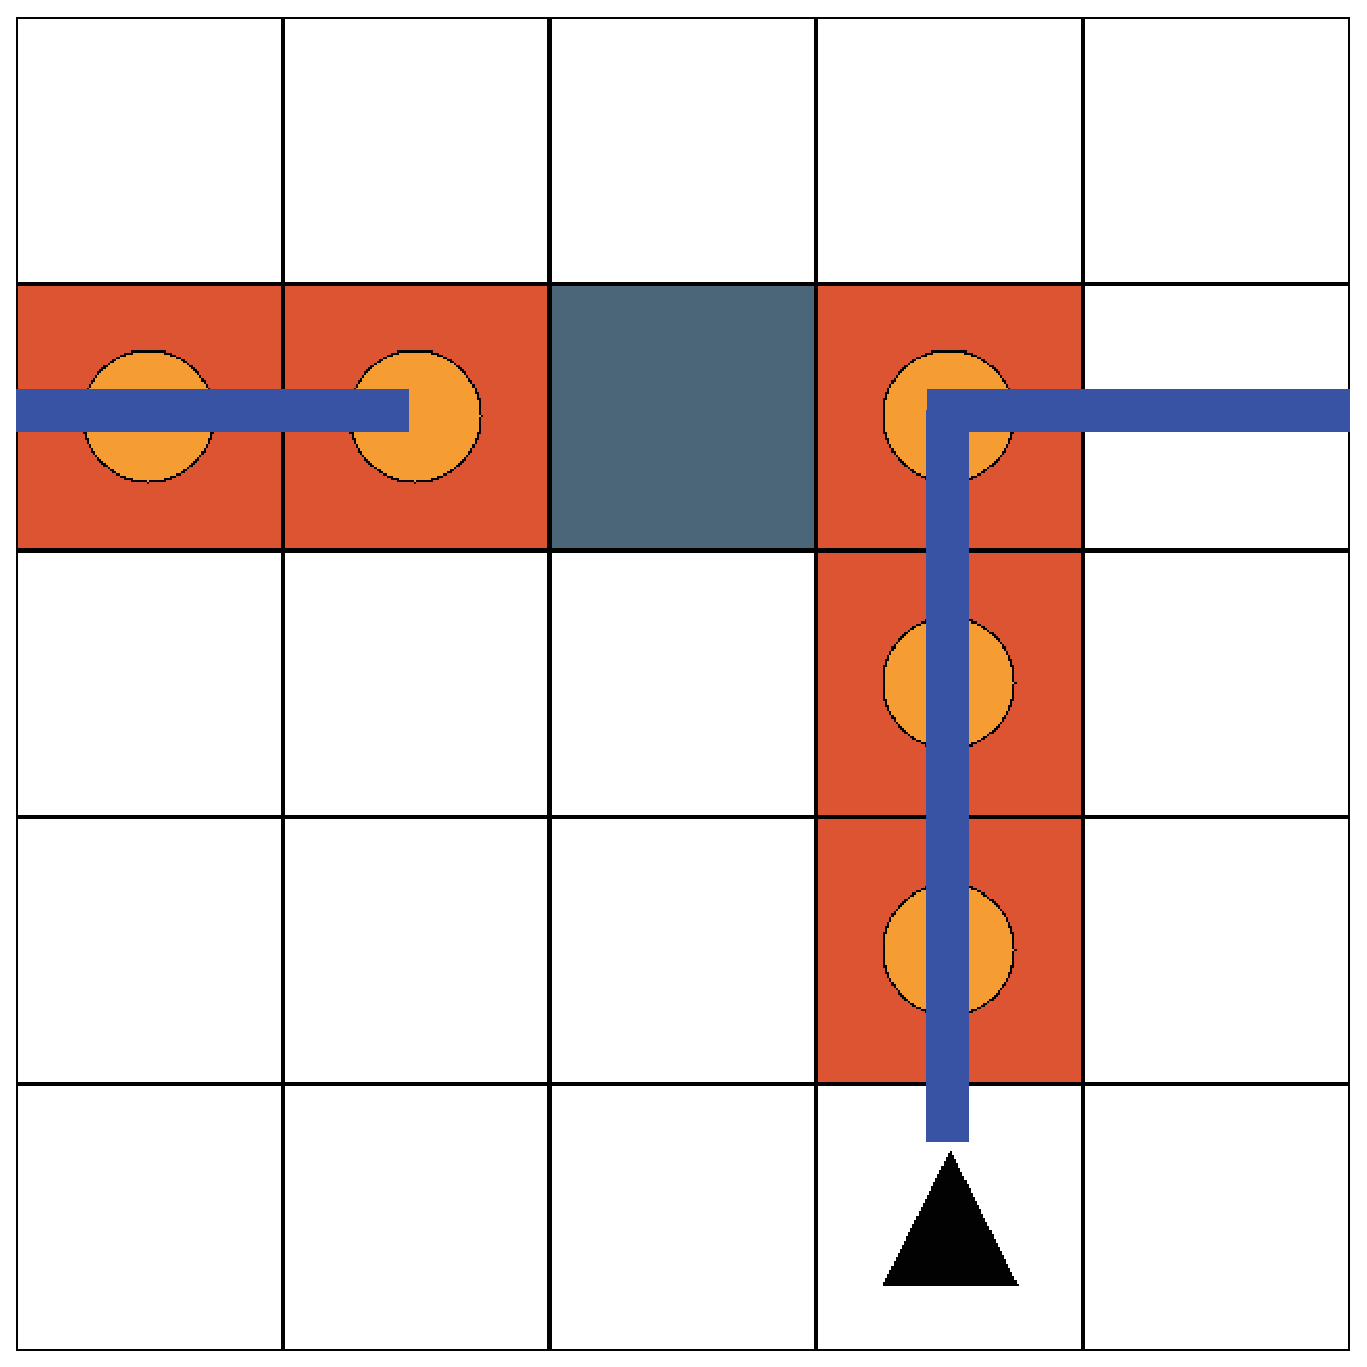
\includegraphics[width=0.25\textwidth]{run39212_t1_gFinal}
\caption[Individual Path in Test Trail 1]{This figure shows the path the best individual took with test trail 1 indicated with the dark line. Note this trail has two optimal paths (left or right at first turn). The particular solution from the \gls{ga} here took the right turn. Video available at \url{http://goo.gl/MUktKs}.}
\label{fig:trail1_final_gen}
\end{figure}

\clearpage
Next, we evaluated test trail 2. Test trail 2 is a slightly more complicated version of test trail 1 featuring two turns, three gaps, and nine pieces of food. This trail is also larger than test trail 1 and the optimal path is to turn left at the first turn versus test trail 1 the agent can turn left or right. This trail was executed with the same configuration with test trail 1 except for allowing twice as many moves, twenty instead of ten. Figure~\ref{fig:trail2_food_consumed} shows how much food the agent consumed and Figure~\ref{fig:trail2_final_gen} shows the path that the final individual took through the maze. Note in this case, the agent actually took extra, unnecessary steps to consume all of the food.

\begin{figure}[ht]
\centering
\begin{tikzpicture}
    \begin{axis}[
    xlabel={Generation},
    ylabel={Food Consumed},
    xticklabel style={/pgf/number format/fixed},
    cycle multi list={Mark-Dark2-4},
    legend style={
        cells={anchor=east},
        legend pos=south east,
    },
    scale only axis, % The height and width argument only apply to the actual axis
    height=7.313cm,
    width=13cm,
    every axis post/.style={
        thick,
    },
    ]
        \addplot table [x=Generations, y=Max, col sep=comma] {data/food_run_39268.csv};
        \addplot table [x=Generations, y=Min, col sep=comma] {data/food_run_39268.csv};
        \addplot table [x=Generations, y=Avg, col sep=comma] {data/food_run_39268.csv};
        \addplot[dashed] table [x=Generations, y=Available, col sep=comma] {data/food_run_39268.csv};
        
        \legend{Max, Min, Avg, Available}
    
    \end{axis}
\end{tikzpicture}
\caption[Food Consumed in Test Trail 2]{Plot of food consumed over each generation on test trail 2. This slightly more complicated trail takes a few more generations, but finds a solution after ten generations.}
\label{fig:trail2_food_consumed}
\end{figure}

\begin{figure}[ht]
\centering
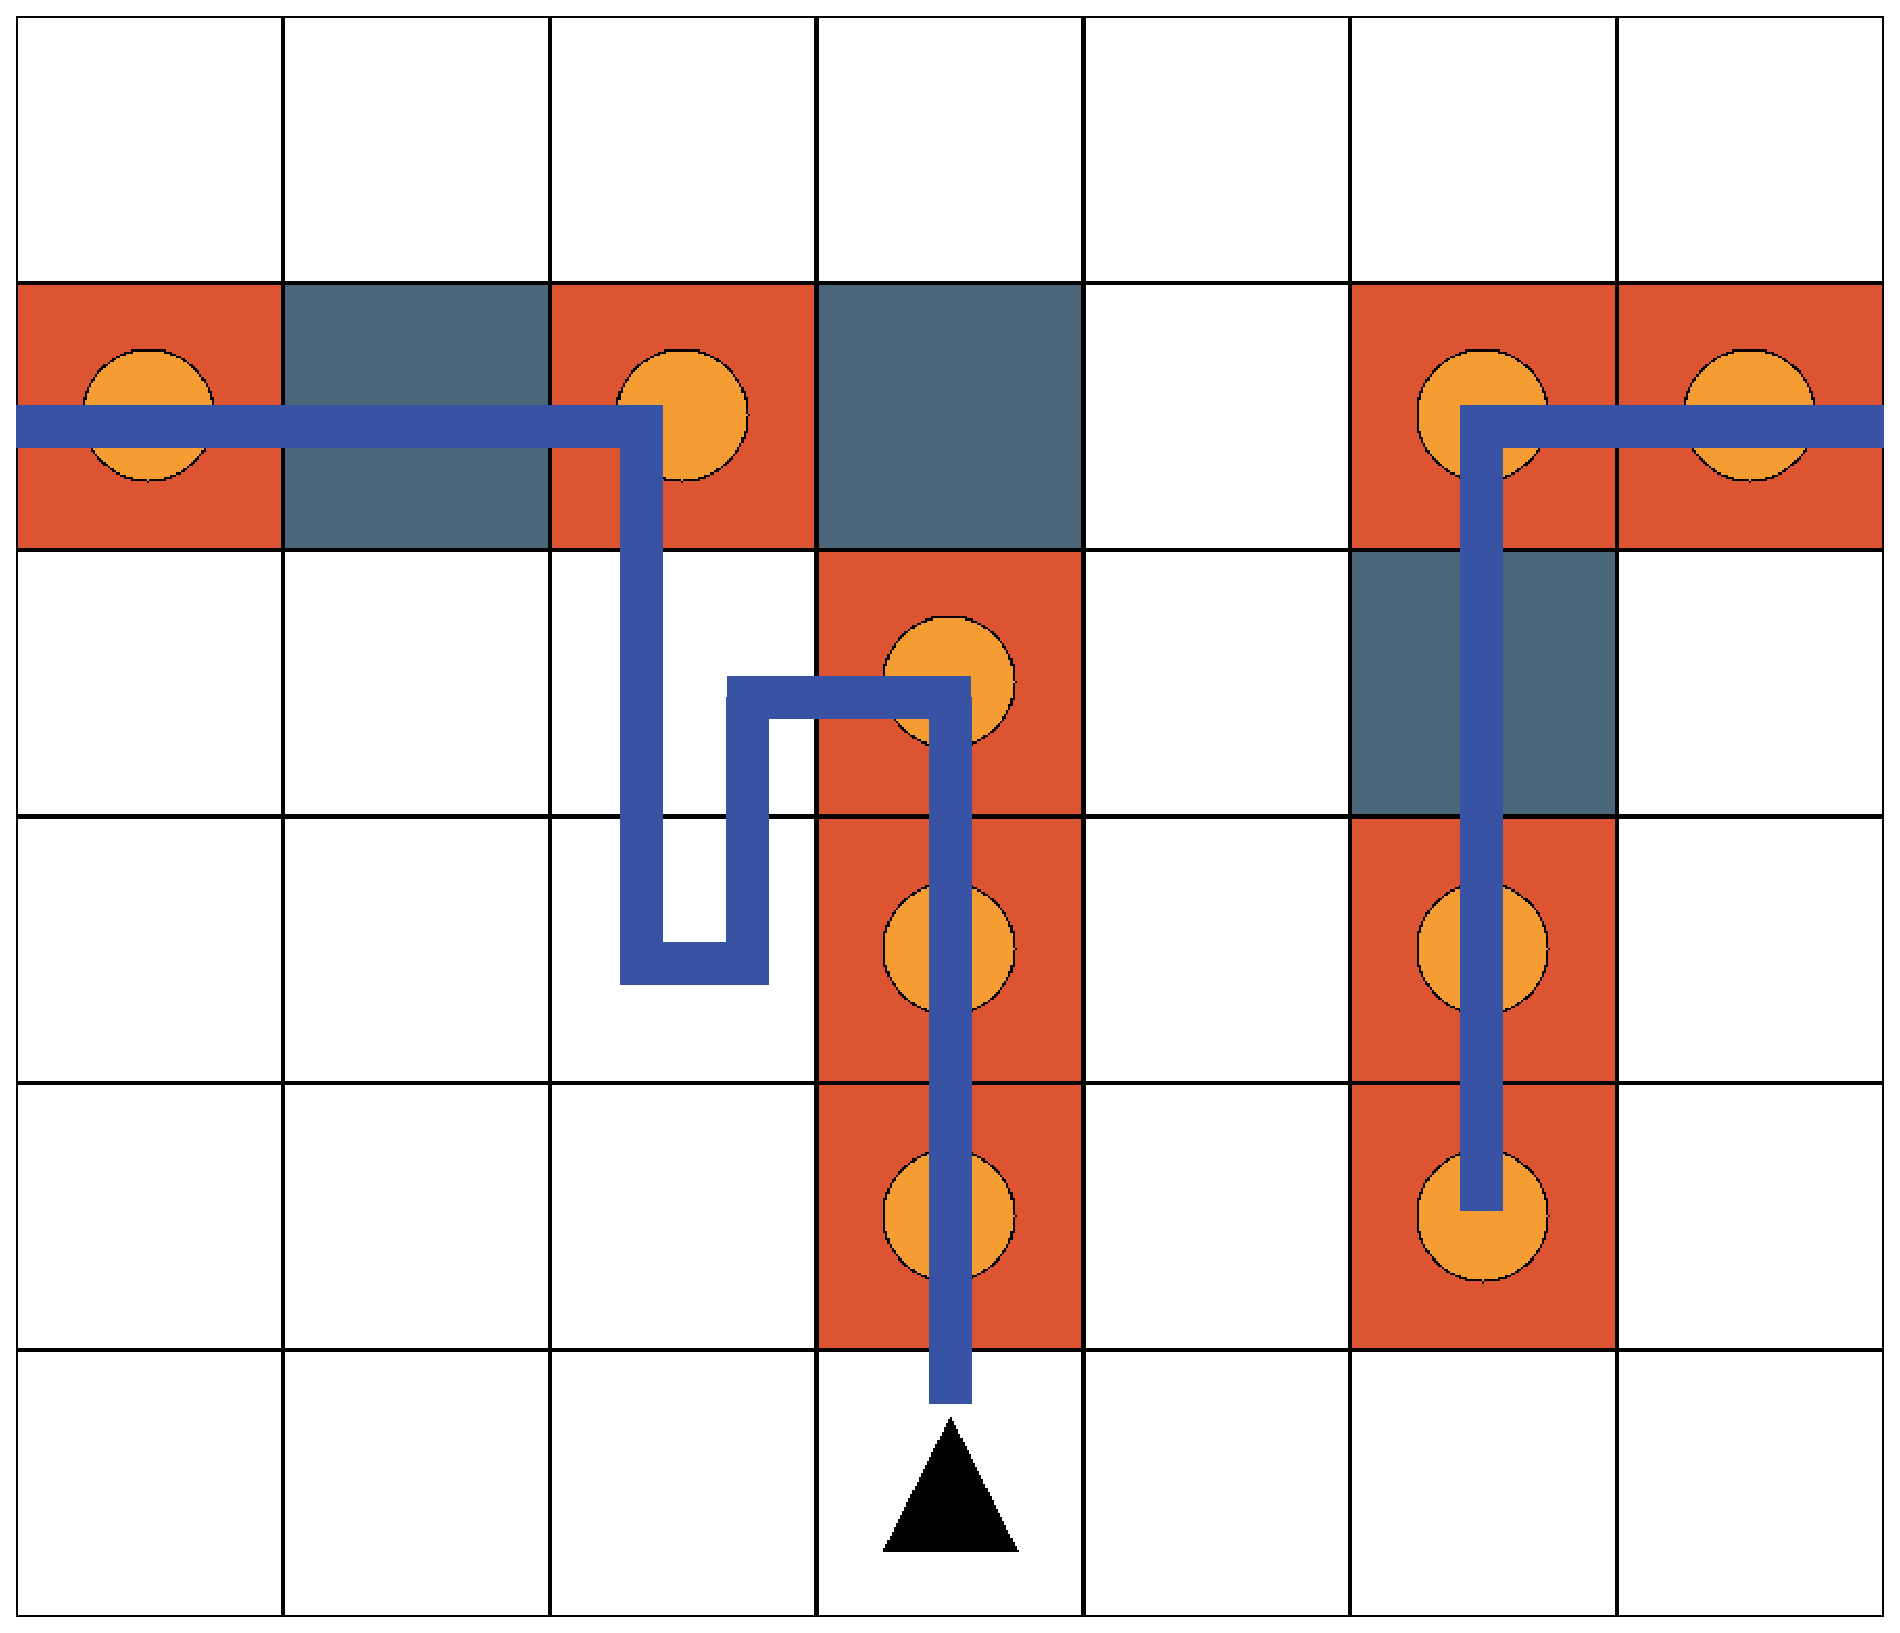
\includegraphics[width=0.25\textwidth]{run39268_t2_gFinal}
\caption[Individual Path in Test Trail 2]{Path of agent consuming food in test trail 2 in final generation. In this case, the ant found a solution consuming all food, but did it with a non-optimal number of moves. As we mentioned before, we stop when a solution that finds all food is found and do not continue to optimize for moves. Video available at \url{http://goo.gl/jDO7p1}.}
\label{fig:trail2_final_gen}
\end{figure}

\clearpage
The next \gls{ga} evaluation was performed on Jefferson's John Muir trail. This is a complicated trail compared to the two test trails and serves as a good starting benchmark for the performance of the \gls{ga}. Figure~\ref{fig:jmt_tr_food_consumed} shows the food consumption over generations. Generation 443 contained an individual that consumed all of the food on the trail. Figure~\ref{fig:jmt_tr_final_gen} shows the path this individual took through the John Muir trail.

\begin{figure}[ht]
\centering
\begin{tikzpicture}
    \begin{axis}[
    xlabel={Generation},
    ylabel={Food Consumed},
    xticklabel style={/pgf/number format/fixed},
    cycle multi list={Mark-Dark2-4},
    legend style={
        cells={anchor=east},
        legend pos=south east,
    },
    scale only axis, % The height and width argument only apply to the actual axis
    height=7.313cm,
    width=13cm,
    mark repeat=20,
    every axis post/.style={
        thick,
    },
    ]
        \addplot table [x=Generations, y=Max, col sep=comma] {data/food_run_39653.csv};
        \addplot table [x=Generations, y=Min, col sep=comma] {data/food_run_39653.csv};
        \addplot table [x=Generations, y=Avg, col sep=comma] {data/food_run_39653.csv};
        \addplot[dashed] table [x=Generations, y=Available, col sep=comma] {data/food_run_39653.csv};
        
        \legend{Max, Min, Avg, Available}
    
    \end{axis}
\end{tikzpicture}
\caption[Food Consumed in John Muir Trail]{Plot showing the consumption of food for each generation on the John Muir trail. This trail took more generations compared to test trail 1 and test trail 2 to reach a solution because of the larger size. It finds a solution after 443 generations.}
\label{fig:jmt_tr_food_consumed}
\end{figure}

\begin{figure}[ht]
\centering
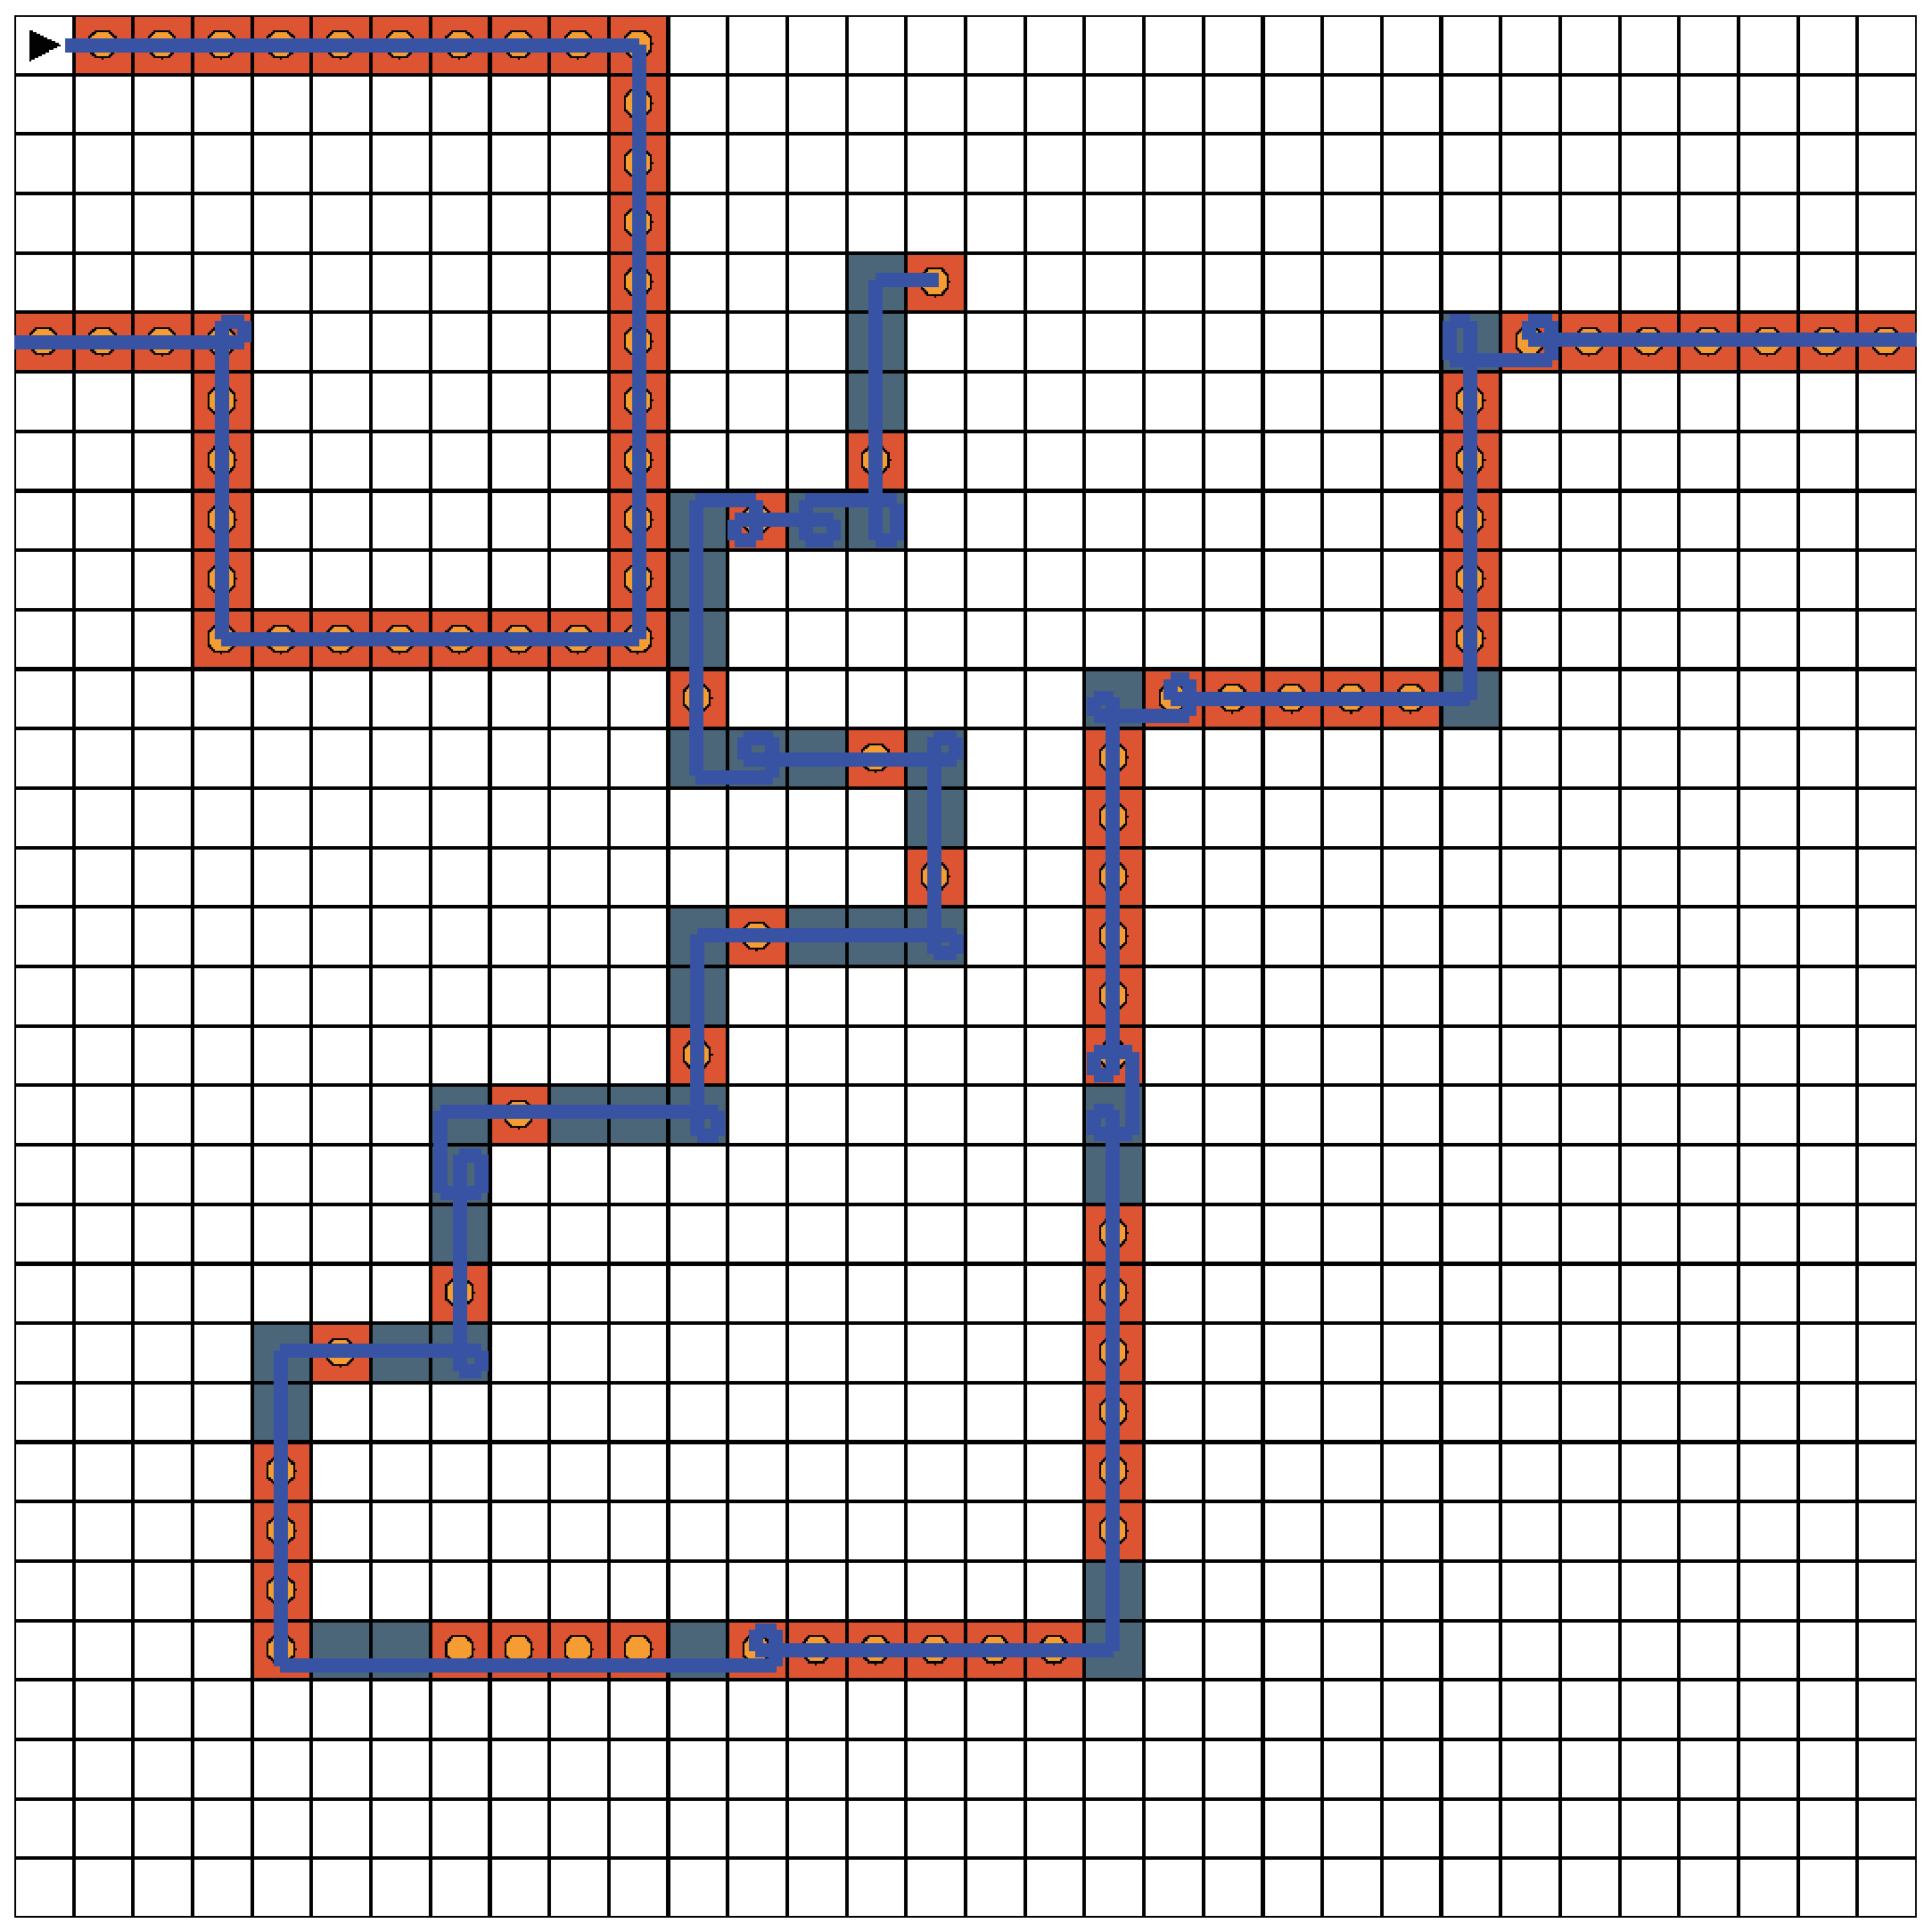
\includegraphics[width=0.95\textwidth]{run39653_t3_gFinal}
\caption[Individual Path in John Muir Trail]{Path of the agent through Santa Fe Trail in final (443) generation. The agent did turn within some squares before moving forward like the first left turn on the trail. This individual required 199 moves and consumed all 89 pieces of food. This individual never took a left turn and only made right turns through the trail. Video available at \url{http://goo.gl/OaGsyh}.}
\label{fig:jmt_tr_final_gen}
\end{figure}

\clearpage
Using the same configuration on the John Muir trail, Figure~\ref{fig:jmt_tr_food_stuck_run} shows an example of a run that was terminated early. This run did not go to completion because there was no change in the standard deviation of the maximum amount of food consumed across the population.

\begin{figure}[ht]
\centering
\begin{tikzpicture}
    \begin{axis}[
    xlabel={Generation},
    ylabel={Food Consumed},
    xticklabel style={/pgf/number format/fixed},
    cycle multi list={Mark-Dark2-4},
    legend style={
        cells={anchor=east},
        legend pos=south east,
    },
    scale only axis, % The height and width argument only apply to the actual axis
    height=7.313cm,
    width=13cm,
    mark repeat=20,
    every axis post/.style={
        thick,
    },
    ]
        \addplot table [x=Generations, y=Max, col sep=comma] {data/food_run_39635.csv};
        \addplot table [x=Generations, y=Min, col sep=comma] {data/food_run_39635.csv};
        \addplot table [x=Generations, y=Avg, col sep=comma] {data/food_run_39635.csv};
        \addplot[dashed] table [x=Generations, y=Available, col sep=comma] {data/food_run_39635.csv};
        
        \legend{Max, Min, Avg, Available}
    
    \end{axis}
\end{tikzpicture}
\caption[Food Consumed in John Muir Trail on Stuck Run]{Plot showing a \gls{ga} run on the John Muir trail that is no longer progressing. This run was terminated early because it did not have a change in the standard deviation of the maximum food conumsed for the previous 300 generations starting at around generation 90. }
\label{fig:jmt_tr_food_stuck_run}
\end{figure}

\clearpage
Now, we will show the results of a performance sweep to see the advantage of using a parallel processing environment, like \gls{scoop}. We performed this evaluation using the Santa Fe Trail and and used the \gls{ga} parameters specified in Table~\ref{tab:testing_run_parameters}. For these trials, we disabled the automatic termination if all food was consumed for a fair comparison. All of these runs ran for the full 100 generations. Then, the number of moves was ran with a value of 100, 200, 300, and 400 across a maximum number of processes of 1, 2, 4, and 8. Figure~\ref{fig:trail_runner_do_benchmark} shows this plot. This benchmark was performed on a DigitalOcean \gls{vps} featuring a 160 GB \gls{ssd}, 16 GB of memory, and an eight core processor~\cite{DigitalOcean_Inc_undated-bc}.

\begin{figure}[ht]
\centering
\begin{tikzpicture}
    \begin{axis}[
    ybar,
    bar width = 0.5cm,
    xlabel={Number of Processes},
    ylabel={Run Time (seconds)},
    legend style={
        cells={anchor=east},
        legend pos=north east,
    },
    scale only axis, % The height and width argument only apply to the actual axis
    symbolic x coords={1, 2, 4, 8},
    enlarge x limits=0.25,
    enlarge y limits=false,
    ymin=0,
    ymax=700,
    xtick=data,
    height=7.313cm,
    width=13cm,
    area legend
    ]
        \addlegendimage{empty legend};
        \addplot [fill={Accent-4-1}] coordinates {(1, 168) (2, 107) (4, 77) (8, 50)};
        
        \addplot [fill={Accent-4-2}, 
            postaction={
                pattern=horizontal lines,
                pattern color=black!50,
            }] coordinates {(1, 317) (2, 193) (4, 116) (8, 81)};
            
        \addplot [fill={Accent-4-3}, postaction={
                pattern=north east lines,
                pattern color=black!50,
            }] coordinates {(1, 468) (2, 266) (4, 167) (8, 108)};
        \addplot [fill={Accent-4-4}, postaction={
                pattern=grid,
                pattern color=black!50,
            }] coordinates {(1, 623) (2, 338) (4, 210) (8, 131)};
        
        \legend{\textbf{Max. Moves}, 100, 200, 300, 400}
    
    \end{axis}
\end{tikzpicture}
\caption[Run Time Benchmark of Trail Runner]{Run time benchmark for trail runner on Santa Fe trail. Benchmark swept the number of processes and maximum number of moves to collect time for each one. Notice how more processes speeds up the simulation and more moves requires more time to process.}
\label{fig:trail_runner_do_benchmark}
\end{figure}

\clearpage
Figure~\ref{fig:sft_none_evidence_plot} shows a run where the ``None'' move option was enabled to show how it is not used by the best individual at the end of the run. This run goes for 89 generations until an individual evolves that consumes all pieces of food. This was performed on the full Santa Fe trail.

\begin{figure}[hbt]
\centering
\begin{tikzpicture}
    \begin{axis}[
    xlabel={Generation},
    ylabel={Number of Moves},
    xticklabel style={/pgf/number format/fixed},
    cycle multi list={Mark-Dark2-4},
    legend style={
        cells={anchor=east},
        legend pos=north east,
        legend columns=2,
    },
    scale only axis, % The height and width argument only apply to the actual axis
    height=7.313cm,
    width=13cm,
    mark repeat=10,
    every axis post/.style={
        thick,
    },
    ]
        \addplot table [x=Generations, y=Left, col sep=comma] {data/moves_dir_run_39527.csv};
        \addplot table [x=Generations, y=Right, col sep=comma] {data/moves_dir_run_39527.csv};
        \addplot table [x=Generations, y=Forward, col sep=comma] {data/moves_dir_run_39527.csv};
        \addplot table [x=Generations, y=None, col sep=comma] {data/moves_dir_run_39527.csv};
        
        \legend{Left, Right, Forward, None}
    
    \end{axis}
\end{tikzpicture}
\caption[Moves Type in Santa Fe Trail]{Plot showing the moves the best individual took over a run of 89 moves where it ended with an individual who consumed all food. Notice how the individuals starting around generation 70 took no ``None'' actions. This individual also evolved a final strategy where it only took left turns. This was a common theme in the Jefferson \gls{ann} solutions.}
\label{fig:sft_none_evidence_plot}
\end{figure}

\clearpage
We next swept the delay line length from $N=2$ up to $N=16$ on each of the three segments of the Santa Fe Trail. Figure~\ref{fig:sft_segment_dl_len_sweeps} shows the results on the food collected by the best individual for each of the three segments and the full Santa Fe trail. This chart is showing the best individual run out of a minimum of 70 \gls{ga} evaluations for every delay line length and every trail segment. There are a minimum of 25 evaluations for each length of the full Santa Fe trail. The values are normalized by dividing the food obtained by the maximum amount of food on the trail.

\begin{figure}[hbt]
\centering
\begin{tikzpicture}
    \begin{axis}[
    xlabel={Delay Line Length},
    ylabel={Norm. Food Consumed},
    xticklabel style={/pgf/number format/fixed},
    cycle multi list={Mark-Dark2-4},
    legend style={
        cells={anchor=east},
        legend pos=south east,
    },
    scale only axis, % The height and width argument only apply to the actual axis
    height=7.313cm,
    width=13cm,
    every axis post/.style={
        thick,
    },
    ]
        \addplot table [x=Delay Line Length, y=max_norm, col sep=comma] {data/sweep_trail17.csv};
        \addplot table [x=Delay Line Length, y=max_norm, col sep=comma] {data/sweep_trail19.csv};
        \addplot table [x=Delay Line Length, y=max_norm, col sep=comma] {data/sweep_trail18.csv};
        \addplot table [x=Delay Line Length, y=max_norm, col sep=comma] {data/sweep_trail5.csv};
        
        \legend{Easy (Segment 1), Medium (Segment 2), Hard (Segment 3), Full Trail}
    
    \end{axis}
\end{tikzpicture}
\caption[Maximum Food Gathered by Varying Delay Line Length]{This plot shows the normalized food gathered by the best individual for a given run with varying delay line lengths. Each segment is a subset of the Santa Fe trail. Values were normalized by dividing the food gathered by maximum available for each trail. Notice how a \gls{mdl} of length 2 or 3 is not sufficient. At length 4, the agent start collecting at least 60\% of the available food for all segments and the full trail. The full trail is a more difficult task compared to the segments because there is a much larger trail to explore provided a larger chance for the agent to make poor moves.}
\label{fig:sft_segment_dl_len_sweeps}
\end{figure}

\clearpage
Figure~\ref{fig:sft_easy_segment_mean_dl_len_sweeps}, Figure~\ref{fig:sft_med_segment_mean_dl_len_sweeps}, Figure~\ref{fig:sft_hard_segment_mean_dl_len_sweeps}, and Figure~\ref{fig:sft_full_segment_mean_dl_len_sweeps} show the normalized mean for the food collected across each \gls{ga} evaluation's best individual. Figure~\ref{fig:sft_all_sweep_no_std} shows all four stacked without error bars. The error bars on each chart represent the standard deviation from the means for the food collected across each \gls{ga} evaluation's best individual. These charts are useful when determining the minimum delay line length for each trail.

\begin{figure}[hbt]
\centering
\begin{tikzpicture}
    \begin{axis}[
    xlabel={Delay Line Length},
    ylabel={Norm. Mean Food Consumed},
    xticklabel style={/pgf/number format/fixed},
    scale only axis, % The height and width argument only apply to the actual axis
    height=7.313cm,
    width=13cm,
    ymin=0.0,
    ymax=1.2,
    every axis post/.style={
        thick,
    },
    ]
        \addplot [{Dark2-4-1}, thick, error bars/.cd, y dir = both, y explicit] 
            table [x=Delay Line Length, y=mean_norm, y error=error_norm, col sep=comma] {data/sweep_trail17.csv};
        
    \end{axis}
\end{tikzpicture}
\caption[Mean Food Gathered on Easy Segment with Varying Delay Line Length]{Plot showing the normalized food gathered with the average of the best individual across each \gls{ga} run on the easy trail segment. Values are normalized by dividing the food gathered by the maximum amount on the trail. Local maximums are at 5 and 12, but the wide standard deviations make it hard to draw conclusions of this chart alone.}
\label{fig:sft_easy_segment_mean_dl_len_sweeps}
\end{figure}

\begin{figure}[hbt]
\centering
\begin{tikzpicture}
    \begin{axis}[
    xlabel={Delay Line Length},
    ylabel={Norm. Mean Food Consumed},
    xticklabel style={/pgf/number format/fixed},
    scale only axis, % The height and width argument only apply to the actual axis
    height=7.313cm,
    width=13cm,
    ymin=0.0,
    ymax=1.2
    ]
        \addplot [{Dark2-4-2}, thick, error bars/.cd, y dir = both, y explicit] 
            table [x=Delay Line Length, y=mean_norm, y error=error_norm, col sep=comma] {data/sweep_trail19.csv};
    
    \end{axis}
\end{tikzpicture}
\caption[Mean Food Gathered on Medium Segment with Varying Delay Line Length]{Plot showing the normalized food gathered with the average of the best individual across each \gls{ga} run on the medium trail segment. Values are normalized by dividing the food gathered by the maximum amount on the trail. There is an overall maximum at length four for this segment with fairly consisent standard deviations.}
\label{fig:sft_med_segment_mean_dl_len_sweeps}
\end{figure}

\begin{figure}[hbt]
\centering
\begin{tikzpicture}
    \begin{axis}[
    xlabel={Delay Line Length},
    ylabel={Norm. Mean Food Consumed},
    xticklabel style={/pgf/number format/fixed},
    scale only axis, % The height and width argument only apply to the actual axis
    height=7.313cm,
    width=13cm,
    ymin=0.0,
    ymax=1.2
    ]
        \addplot [{Dark2-4-3}, thick, error bars/.cd, y dir = both, y explicit] 
            table [x=Delay Line Length, y=mean_norm, y error=error_norm, col sep=comma] {data/sweep_trail18.csv};
    
    \end{axis}
\end{tikzpicture}
\caption[Mean Food Gathered on Hard Segment with Varying Delay Line Length]{Plot showing the normalized food gathered with the average of the best individual across each \gls{ga} run on the hard trail segment. Values are normalized by dividing the food gathered by the maximum amount on the trail. There is a local maximum around 6, 10, and 16 for these lengths. Note that wide standard deviation through for the majority of these values, in particular at length 4.}
\label{fig:sft_hard_segment_mean_dl_len_sweeps}
\end{figure}

\begin{figure}[hbt]
\centering
\begin{tikzpicture}
    \begin{axis}[
    xlabel={Delay Line Length},
    ylabel={Norm. Mean Food Consumed},
    xticklabel style={/pgf/number format/fixed},
    scale only axis, % The height and width argument only apply to the actual axis
    height=7.313cm,
    width=13cm,
    ymin=0.0,
    ymax=1.2
    ]
        \addplot [{Dark2-4-4}, thick, error bars/.cd, y dir = both, y explicit] 
            table [x=Delay Line Length, y=mean_norm, y error=error_norm, col sep=comma] {data/sweep_trail5.csv};

    \end{axis}
\end{tikzpicture}
\caption[Mean Food Gathered on Santa Fe Trail with Varying Delay Line Length]{Plot showing the normalized food gathered with the average of the best individual across each \gls{ga} run on the full Santa Fe trail. Values are normalized by dividing the food gathered by the maximum amount on the trail. There is a local maximum around delay line length 4, 6, 11, and 13 in this figure. This chart also shows a wider standard deviation for a delaly line of length 4, as seen in the maximums for this trail (Figure~\ref{fig:sft_segment_dl_len_sweeps}).}
\label{fig:sft_full_segment_mean_dl_len_sweeps}
\end{figure}

\begin{figure}[hbt]
\centering
\begin{tikzpicture}
    \begin{axis}[
    xlabel={Delay Line Length},
    ylabel={Norm. Mean Food Consumed},
    xticklabel style={/pgf/number format/fixed},
    scale only axis, % The height and width argument only apply to the actual axis
    cycle multi list={Mark-Dark2-4},
    height=7.313cm,
    width=13cm,
    ymin=0.0,
    ymax=1.2,
    every axis post/.style={
        thick,
    },
    legend style={
        cells={anchor=east},
        legend pos=south east,
    },
    ]
        \addplot 
            table [x=Delay Line Length, y=mean_norm, col sep=comma] {data/sweep_trail17.csv};
        
        \addplot  
            table [x=Delay Line Length, y=mean_norm, col sep=comma] {data/sweep_trail19.csv};
        
        \addplot
            table [x=Delay Line Length, y=mean_norm, col sep=comma] {data/sweep_trail18.csv};
            
        \addplot
            table [x=Delay Line Length, y=mean_norm, col sep=comma] {data/sweep_trail5.csv};            
        \legend{Easy (Segment 1), Medium (Segment 2), Hard (Segment 3), Full Trail}
        
    \end{axis}
\end{tikzpicture}
\caption[Mean Food Gathered on All Segments with Varying Delay Line Length]{Plot showing the normalized food gathered with the average of the best individual across each \gls{ga} run for all trail segments. Values are normalized by dividing the food gathered by the maximum amount on the trail. There is not a consistent local maximum for all the trails, but all trails have a sizeable increase in performance from length 3 to 4.}
\label{fig:sft_all_sweep_no_std}
\end{figure}


\clearpage
\section{Discussion}
Test trail 1, test trail 2, and the John Muir trail all found a solution consuming all food on the trails through the \gls{ga} configuration as shown in Figure~\ref{fig:trail1_food_consumed}, Figure~\ref{fig:trail2_food_consumed}, and Figure~\ref{fig:jmt_tr_food_consumed}, respectively. The criteria for a solution in this case was to consume all of the food within the specified number of moves without regard to optimization of number of moves through the trail. As a result, the path the agent took in test trail 2 (Figure~\ref{fig:trail2_final_gen}) and the John Muir trail (Figure~\ref{fig:jmt_tr_final_gen}) are both valid solutions, but not necessarily the most efficient means through the trail. Because the simplicity of test trail 1, the agent actually found an optimal solution in Figure~\ref{fig:trail1_final_gen}.

Figure~\ref{fig:jmt_tr_food_stuck_run} shows an evaluation that was no longer progressing after around generation 90. This evaluation shows how some runs are terminated early in the non-\gls{crn} simulations because the population of individuals grows stale. Even with further mutation and crossover, which is occurring in this diagram, there is no longer variation in the population after 300 generations. As such, this particular run as well many of the others used in our testing were terminated in a similar fashion.

The benchmark on the Santa Fe trail also show the importance of \gls{scoop} in the evaluation of these tasks. Without some form of parallelism, the evaluation of the \gls{ga} (as expected) takes more than three times as long with 400 moves on the Santa Fe trail (see Figure~\ref{fig:trail_runner_do_benchmark}). There is an upper bound on the amount of gain which is practically the population size. The maximum number of parallel tasks we could ever have on this task is the size of the population. This is because the fitnesses of the entire population and offspring must be evaluated prior to entering the selection phase.

Figure~\ref{fig:sft_none_evidence_plot} confirms that removal of the no move option was not an issue for the \gls{ann}. Jefferson and Koza both observed the same behavior~\cite{Jefferson1992-ph}~\cite{Koza1992-xs}. Like this chart, they both found that the elite individuals at the end of a simulation would have never used the no move option. A second common theme here is this individual made no right turns. Very often, the elite individuals would eventually evolve to only make left or right turns throughout the trail. Figure~\ref{fig:jmt_tr_final_gen} shows an individual who only made right turns throughout the John Muir trail.

The next chart, Figure~\ref{fig:sft_segment_dl_len_sweeps} shows how we arrived at the desired length of delay line for implementation in a \gls{crn}. All four trails agree that a delay line of length two or three is insufficient to solve the task. At length four, the easy trail hits the first point that it is capable of consuming all the food. In addition, the hard trail and the medium trail also make a large jump between the values on a delay line of length three. The same jump occurs on the full Santa Fe trail for the length of the delay line. The objective is to find the \textit{least complex} trail that will consume the maximum amount of food. From the maximum chart alone, the conclusion that a length four is sufficient is drawn for the easy, hard, and full Santa Fe trail. The medium trail requires more investigation because at first glance, it appears a delay line of length six is the best choice.

Notice the medium trail's best performance, on average (see Figure~\ref{fig:sft_med_segment_mean_dl_len_sweeps}), occurs when the delay line of length equals four. This is confirmed looking at the standard deviation showing that the deviation is lower compared to that of a delay line length six. With this data, the conclusion that a delay line of length equals four, on average, will perform better than a delay line of length six on the medium trail. Using the mean and standard deviation, the results conclude that a delay line length of four is sufficient across all trails to consume the most amount of food from these results. In the next chapter, we now take this delay line length of $N=4$ and move it into a \gls{crn}.


\glsresetall
\chapter{Chemical Reaction Network Trail Simulations}
\label{chap:trail_simulations}
In this chapter, we discuss how we integrated the delay line with an \gls{ann} to solve the navigation of an agent through modified versions of the Santa Fe trails in a \gls{crn}. We carry over the \gls{ga} shown in the previous chapter and the minimal delay line length of $N=4$ to implement them as a \gls{crn}. We will also show in here that the increased run time of a \gls{crn} versus a non-\gls{crn} makes the optimization prior to going to a \gls{crn} an important step. 

This chapter starts out by discussing the methodology we used to gather the data, presents the results, and then provides a discussion on the data presented.

\section{Methodology}
After finding the minimal length of delay line in the non-\gls{crn} simulations, we moved with this length of $N=4$ into the \gls{crn} simulations. We performed these simulations represented in a \gls{crn} with \gls{coel}~\cite{Banda2014-qw}. Each trail and \gls{ann} was evaluated 10 or more times in \gls{coel}. The \gls{crn} \gls{ann} was constructed with a network similar to the one in Figure~\ref{fig:trail_ann_w_dl2} with a few differences. 

Figure~\ref{fig:chem_trail_ann_dl4} shows an example of this modified neural network for the chemistry simulations. The node model we use in the \gls{crn} does not require the inverted input so there is a single input node for each delay line stage. Another exception is the presence of a hidden perceptron. We wanted to evaluate performance to see if the hidden perceptron was necessary in the \gls{ann} in Figure~\ref{fig:trail_ann_w_dl2}. We evaluated performance both with the presence of a hidden layer (a single perceptron) and without a hidden layer completely.

\begin{figure}
\centering
\begin{tikzpicture}[->,draw=black!100, node distance=\layerseptikznn]
    % Based off code form http://www.texample.net/tikz/examples/neural-network/
    \tikzstyle{every pin edge}=[<-,shorten <=1pt]
    \tikzstyle{neuron}=[circle,draw=black!50,fill=white!25,minimum size=25pt,inner sep=0pt]
    \tikzstyle{input neuron}=[neuron, draw=black!50, fill=Accent-5-1];
    \tikzstyle{output neuron}=[neuron, draw=black!50, fill=Accent-5-3];
    \tikzstyle{blank neuron}=[neuron, draw=white!50, fill=white!50];
    \tikzstyle{hidden neuron}=[neuron, draw=black!50, fill=Accent-5-2];
    \tikzstyle{annot} = [text width=4em, text centered]
    \tikzstyle{dlbox}=[rectangle,draw=black!50,fill=Accent-5-4];
    \tikzstyle{input value}=[circle,draw=black!50,fill=Accent-5-5!50,minimum size=25pt,inner sep=0pt];

    % Draw the input layer nodes
    \node[input neuron] (I-1) at (0,-2) {};
    \node[input neuron] (I-2) at (0,-3) {};
    \node[input neuron] (I-3) at (0,-4) {};
    \node[input neuron] (I-4) at (0,-5) {};
    
    % Draw the delay line
    \node[input value] (X-1) at (-\layerseptikznn, -1) {X};
    \node[dlbox] (DL-1) at (-\layerseptikznn, -2) {X[0]};
    \node[dlbox] (DL-2) at (-\layerseptikznn, -3) {X[-1]};
    \node[dlbox] (DL-3) at (-\layerseptikznn, -4) {X[-2]};
    \node[dlbox] (DL-4) at (-\layerseptikznn, -5) {X[-3]};
    
    % Connect the delay line to itself and the input layer.
    \draw[->, draw=black!100] (X-1) edge (DL-1);
    \draw[->, draw=black!100] (DL-1) edge (DL-2);
    \draw[->, draw=black!100] (DL-2) edge (DL-3);
    \draw[->, draw=black!100] (DL-3) edge (DL-4);
    
    \draw[->, draw=black!100] (DL-1) edge (I-1);
    \draw[->, draw=black!100] (DL-2) edge (I-2);
    \draw[->, draw=black!100] (DL-3) edge (I-3);
    \draw[->, draw=black!100] (DL-4) edge (I-4);
            
    
    % Draw the hidden layer nodes
        \path[yshift=0.5cm]
            node[hidden neuron] (H-1) at (\layerseptikznn, -4) {H1};

    % Draw the output layer node
        \path node[output neuron, pin={[pin edge={->}]right:Forward}] 
                (O-2) at (\layerseptikznn * 2, -2) {};
        \path node[output neuron, pin={[pin edge={->}]right:Left}] 
                (O-3) at (\layerseptikznn * 2, -3) {};
        \path node[output neuron, pin={[pin edge={->}]right:Right}] 
                (O-4) at (\layerseptikznn * 2, -4) {};
        \path node[blank neuron] 
                (O-5) at (\layerseptikznn * 2, -5) {};

    % Connect every node in the input layer with every node in the
    % hidden layer.
    \foreach \source in {1,...,4}
            \path (I-\source) edge (H-1);
            
    \draw[-, draw=violet!100, thick](I-1) -- ($ (I-1) !.75! (O-2) $);
    \draw[-, draw=violet!100, thick](I-2) -- ($ (I-2) !.75! (O-3) $);
    \draw[-, draw=violet!100, thick](I-3) -- ($ (I-3) !.75! (O-4) $);
    \draw[-, draw=violet!100, thick](I-4) -- ($ (I-4) !.75! (O-5) $);
            
    \foreach \dest in {2,...,4}{
        \draw[->, draw=violet!100] ($ (I-1) !.75! (O-2) $) -- (O-\dest.west);
        \draw[->, draw=violet!100] ($ (I-2) !.75! (O-3) $) -- (O-\dest.west);
        \draw[->, draw=violet!100] ($ (I-3) !.75! (O-4) $) -- (O-\dest.west);
        \draw[->, draw=violet!100] ($ (I-4) !.75! (O-5) $) -- (O-\dest.west);
    }

    % Connect every node in the hidden layer with the output layer
    \foreach \dest in {2,...,4}
        \path (H-1) edge (O-\dest);

    % Annotate the layers
    \node[annot,above of=H-1, node distance=3cm] (hl) {Hidden layer};
    \node[annot,left of=hl] {Input layer};
    \node[annot,right of=hl] {Output layer};
\end{tikzpicture}
\caption[Delay Line with ANN in Chemistry]{This figure shows the \gls{ann} combined with a 4-input ($N=4$) delay line (on left). This feedforward \gls{ann} has full connections from the input to the hidden layer, input to the output layer, and hidden to the output layer. The delay line has a single input neuron for each stage in a chemistry. Values shift down the delay line where $X[0]$ represents the current input, $X[-1]$ represents the previous input, and so on.}
\label{fig:chem_trail_ann_dl4}
\end{figure}

The perceptrons were modeled with Banda's \gls{aasp}~\cite{Banda2014-kg} and the \gls{ann} in a chemistry was modeled after Blout's compartmental chemistries~\cite{Blount_undated-ro}. Using these two systems allowed us to construct a network that is comparable to the one in Figure~\ref{fig:trail_ann_w_dl2} and the current state of the art in a \gls{crn}. Further simplification from Figure~\ref{fig:trail_ann_w_dl2} is possible because there is a single connection from the delay line to the input layer, so we remove the formal perceptron layer and have the delay line itself act as the input layer as shown in Figure~\ref{fig:chem_comp_dl4}. Each of the nodes in this diagram are represented with a four or five input \gls{aasp}. Table~\ref{tab:aasp_react} shows the reactions and rate constants of the \gls{aasp} used to model these perceptrons. The \gls{mdl} reactions and rates are extended as discussed in Chapter~\ref{chap:delay_line} and are shown earlier in Table~\ref{tab:rateconstantsMan}. With the modified input layer, this means the total number of nodes in the \gls{crn} \gls{ann} is four with a hidden neuron and three without a hidden neuron.

\begin{figure}
\centering
\begin{tikzpicture}[->,draw=black!100, node distance=\layerseptikznn]
    % Based off code form http://www.texample.net/tikz/examples/neural-network/
    \tikzstyle{every pin edge}=[<-,shorten <=1pt]
    \tikzstyle{neuron}=[circle,draw=black!50,fill=white!25,minimum size=25pt,inner sep=0pt]
    \tikzstyle{input neuron}=[neuron, draw=black!50, fill=Accent-5-1];
    \tikzstyle{output neuron}=[neuron, draw=black!50, fill=Accent-5-3];
    \tikzstyle{blank neuron}=[neuron, draw=white!50, fill=white!50];
    \tikzstyle{hidden neuron}=[neuron, draw=black!50, fill=Accent-5-2];
    \tikzstyle{annot} = [text width=4em, text centered]
    \tikzstyle{dlbox}=[rectangle,draw=black!50,fill=Accent-5-4];
    \tikzstyle{input value}=[circle,draw=black!50,fill=Accent-5-5!50,minimum size=25pt,inner sep=0pt];
    
    % Draw the delay line
    
    \node[input value] (X) at (-\layerseptikznn,-2) {X};
    \node[dlbox] (I-1) at (0, -2) {X[0]};
    \node[dlbox] (I-2) at (0, -4) {X[-1]};
    \node[dlbox] (I-3) at (0, -6) {X[-2]};
    \node[dlbox] (I-4) at (0, -8) {X[-3]};
    \node[scale=0.2]	(syr1) [above right=-0.1cm of X] {\syringePDFImage};
    
    % Connect the delay line to itself.
    \draw[->, draw=black!100] (X) edge (I-1);
    \draw[->, draw=black!100] (I-1) edge (I-2);
    \draw[->, draw=black!100] (I-2) edge (I-3);
    \draw[->, draw=black!100] (I-3) edge (I-4);
            
    
    % Draw the hidden layer nodes
        \path[yshift=0.5cm]
            node[hidden neuron] (H-1) at (\layerseptikznn, -5.5) {AASP4};

    % Draw the output layer node
        \path node[output neuron, pin={[pin edge={->}]right:Forward}] 
                (O-2) at (\layerseptikznn * 2, -2) {AASP5};
        \path node[output neuron, pin={[pin edge={->}]right:Left}] 
                (O-3) at (\layerseptikznn * 2, -4) {AASP5};
        \path node[output neuron, pin={[pin edge={->}]right:Right}] 
                (O-4) at (\layerseptikznn * 2, -6) {AASP5};
        \path node[blank neuron] 
                (O-5) at (\layerseptikznn * 2, -8) {};

    % Connect every node in the input layer with every node in the
    % hidden layer.
    \foreach \source in {1,...,4}
            \path (I-\source) edge (H-1);
            
    \draw[-, draw=violet!100, thick](I-1) -- ($ (I-1) !.6! (O-2) $);
    \draw[-, draw=violet!100, thick](I-2) -- ($ (I-2) !.6! (O-3) $);
    \draw[-, draw=violet!100, thick](I-3) -- ($ (I-3) !.6! (O-4) $);
    \draw[-, draw=violet!100, thick](I-4) -- ($ (I-4) !.6! (O-5) $);
            
    \foreach \dest in {2,...,4}{
        \draw[->, draw=violet!100] ($ (I-1) !.6! (O-2) $) -- (O-\dest.west);
        \draw[->, draw=violet!100] ($ (I-2) !.6! (O-3) $) -- (O-\dest.west);
        \draw[->, draw=violet!100] ($ (I-3) !.6! (O-4) $) -- (O-\dest.west);
        \draw[->, draw=violet!100] ($ (I-4) !.6! (O-5) $) -- (O-\dest.west);
    }

    % Connect every node in the hidden layer with the output layer
    \foreach \dest in {2,...,4}
        \path (H-1) edge (O-\dest);

    % Annotate the layers
    \node[annot,above of=I-1, node distance=2cm] (mdla) {MDL4 (Input)};
    \node[annot,right of=mdla] (hla) {Hidden Layer};
    \node[annot,right of=hla] {Output layer};
\end{tikzpicture}
\caption[Chemical Implementation with AASP]{This figure shows the actual model of the neural network simulated in a chemistry. The evolved parameters were the weights indicated by each individual between nodes. The AASP4 and AASP5 are the Banda's \gls{aasp} and the left input column of $X[n]$ boxes represent the length 4 \gls{mdl}. The syringe on $X$ is the input to the system. Compared to Figure~\ref{fig:chem_trail_ann_dl4}, the single connection between the delay line and input layer allows us to directly connect to the two in our \gls{crn}.}
\label{fig:chem_comp_dl4}
\end{figure}

\begin{table}[ht]
\centering
\begin{tabular}{lcc||lcc}
\textbf{Reaction}                                 & \textbf{Rate} & $\boldsymbol{K_{m}}$ & \textbf{Reaction}                                       & \textbf{Rate} & $\boldsymbol{K_{m}}$\\ \hline
$S_{in} + Y \rightarrow$                          & 0.1800        & (None)               & $X_3 + Y \rightarrow$                                   & 0.3905        & (None) \\
$S_{in} \xrightarrow{W_0} S_{in}Y + Y$            & 2.5336        & 0.5521               & $X_3 \xrightarrow{W_3} X_3Y + Y$                        & 0.1227        & 0.4358 \\
$X_{1} + Y \rightarrow$                           & 0.3905        & (None)               & $W^{\ominus} \xrightarrow{X_3Y} W_3^{\ominus}$          & 1.6788        & 0.1889 \\
$X_{1} \xrightarrow{W_1} X_{1}Y + Y$              & 0.1227        & 0.4358               & $W_3 + W_3^{\ominus} \rightarrow$                       & 0.2416        & (None) \\
$X_{2} + Y \rightarrow$                           & 0.3905        & (None)               & $W^{\oplus} \xrightarrow{X_3Y} W_3$                     & 5.0000        & 0.2744 \\
$X_{2} \xrightarrow{W_2} X_{2}Y + Y$              & 0.1227        & 0.4358               & $X_4 + Y \rightarrow$                                   & 0.3905        & (None) \\
$T \xrightarrow{S_L} E^{\oplus}$                  & 1.9613        & 0.1155               & $X_4 \xrightarrow{W_4} X_4Y + Y$                        & 0.1227        & 0.4358 \\
$Y \xrightarrow{S_L} E^{\ominus}$                 & 1.9613        & 0.1155               & $W^{\ominus} \xrightarrow{X_4Y} W_4^{\ominus}$          & 1.6788        & 0.1889 \\
$T + Y \rightarrow$                               & 5.0000        & (None)               & $W_4 + W_4^{\ominus} \rightarrow$                       & 0.2416        & (None) \\
$W^{\ominus} \xrightarrow{S_{in}Y} W_0^{\ominus}$ & 1.6697        & 0.6000               & $W^{\oplus} \xrightarrow{X_4Y} W_4$                     & 5.0000        & 0.2744 \\
$W_0 + W_0^{\ominus} \rightarrow$                 & 0.2642        & (None)               & $X_5 + Y \rightarrow$                                   & 0.3905        & (None) \\
$W^{\oplus} \xrightarrow{S_{in}Y} W_0$            & 2.9078        & 0.5023               & $X_5 \xrightarrow{W_5} X_5Y + Y$                        & 0.1227        & 0.4358 \\
$W^{\ominus} \xrightarrow{X_{1}Y} W_1^{\ominus}$  & 1.6788        & 0.1889               & $W^{\ominus} \xrightarrow{X_5Y} W_5^{\ominus}$          & 1.6788        & 0.1889 \\
$W_1 + W_1^{\ominus} \rightarrow$                 & 0.2416        & (None)               & $W_5 + W_5^{\ominus} \rightarrow$                       & 0.2416        & (None) \\
$W^{\oplus} \xrightarrow{X_{1}Y} W_1$             & 5.0000        & 0.2744               & $W^{\oplus} \xrightarrow{X_5Y} W_5$                     & 5.0000        & 0.2744 \\
$W^{\ominus} \xrightarrow{X_{2}Y} W_2^{\ominus}$  & 1.6788        & 0.1889               & $B \xrightarrow{E^{\oplus}} E^{\oplus} + W^{\oplus}$    & 1.0000        & 1.0000 \\
$W_2 + W_2^{\ominus} \rightarrow$                 & 0.2416        & (None)               & $B \xrightarrow{E^{\ominus}} E^{\ominus} + W^{\ominus}$ & 1.0000        & 1.0000 \\
$W^{\oplus} \xrightarrow{X_{2}Y} W_2$             & 5.0000        & 0.2744               & $E^{\ominus} + E^{\oplus} \rightarrow$                  & 5.0000        & (None) \\
$Y \xrightarrow{S_F} F$                           & 0.1000        & 3.0000               & ~                                                       & ~             & ~
\end{tabular}
\caption[AASP Reaction Set]{This table shows the reactions and rate constants for the \gls{aasp}. The ``Rate'' column shows the forward reaction rate and ``$K_m$'' shows the catalyst rate. The catalyst is the species shown above the arrow. This table shows an \gls{aasp} with five inputs. Removing the reactions containing $W_5$ and $X_5$ make this a four input \gls{aasp}. Notice how each input ($X_n$) is ``weighed'' like a classical perceptron through varying concentrations of weights ($W_n$). Each $W_n$ is the concentration that was set to a random starting value and then varied during the \gls{ga} process in the \gls{crn}. These reactions are based off work from Banda and Teuscher~\cite{Banda2014-pf}.}
\label{tab:aasp_react}
\end{table}

We chose to represent the delay line in a \gls{crn} with a \gls{mdl}. We did not simulate the system with a \gls{bpl} because the average error for a \gls{bpl} of over two stages is significant compared to a \gls{mdl} of the delay length (see Section~\ref{sec:dl_paper_over_two_stages}). The additional complication of having to manually signal copy between stages of the \gls{mdl} was not a concern for our testing. We were not constrained with the number of inputs and outputs we can have, like other chemical systems.

After finding the best set of \gls{crn} \gls{ann} structures, we wanted to find if the resulting \gls{ann} for that particular trail is specialized or is a generalized solution to these types of tasks. We take the best individual from each trail and then evaluate it on the three other trails as well as Jefferson's John Muir trail (see Figure~\ref{fig:johnmuirtrailimage}) and measure the food consumed. As an example, for the easy trail, we take that individual and run it on the medium, hard, full Santa Fe trail, and full John Muir trail to compare the results. The John Muir trail was limited to 200 moves to match Jefferson's evaluations on the trail where he successfully evolved an \gls{ann} that consumed 89 pieces~\cite{Jefferson1992-ph}.

\clearpage
\section{Results}
In the previous chapter, we arrived at the conclusion that a delay line of length $N=4$ is sufficient for this task. We mention that the segments were used because they ran faster than the full Santa Fe trail. Figure~\ref{fig:coel_time_benchmark} show the run time for a selected run for all three segments and then run time for the full Santa Fe trail in a \gls{crn} with a \gls{mdl} of length $N=4$. 

\begin{figure}[hbt]
\centering
\begin{tikzpicture}
  \begin{axis}[
    ybar,
    xlabel={Santa Fe Trail Type},
    ylabel={Run Time (hours)},
    enlargelimits=0.15,
    symbolic x coords={Easy, Medium, Hard, Full},
    xtick=data,
    height=7cm,
    width=12cm,
    bar width = 0.75cm,
    nodes near coords,
    nodes near coords align={vertical},
    ]
        \addplot [fill={Accent-4-1}] coordinates {(Easy, 3.98) (Medium, 4.42) (Hard, 4.23) (Full, 15.0)};
        
    \end{axis}
\end{tikzpicture}
\caption[COEL Run Time Benchmark]{Plot showing the run time for each of the trail segments for a full run of 100 generations. Notice how the 400 maximum number of moves causes the full Santa Fe trail to take a much longer time than the four other trail segments that only have a maximum moves of 100.}
\label{fig:coel_time_benchmark}
\end{figure}

We also show a table of the first ten generations of a full Santa Fe trail run in Figure~\ref{fig:coel_benchmark_chart} and Table~\ref{tab:coel_benchmark_times}. Each run was executed with the same \gls{ga} parameters and same \gls{crn}. The only difference was the changing trails and the full Santa Fe trail had a maximum moves of 400 compared to the typical 100 for each of the segments. These 300 additional moves cause the time for the full trail execution to be approximately 3.5 times longer than the three trail segments.

\begin{figure}[ht]
\centering
\begin{tikzpicture}
    \begin{axis}[
    ybar,
    xlabel={Generation},
    ylabel={Run Time (min)},
    xticklabel style={/pgf/number format/fixed},
    cycle multi list={Mark-Dark2-4},
    legend style={
        cells={anchor=east},
        legend pos=outer north east,
    },
    scale only axis, % The height and width argument only apply to the actual axis
    height=7.313cm,
    width=13cm,
    ]

        \addplot[fill={Accent-5-1}] plot coordinates {
        (1, 3.75)
        (2, 6.02)
        (3, 11.92)
        (4, 8.85)
        (5, 8.77)
        (6, 3.9)
        (7, 8.62)
        (8, 7.25)
        (9, 3.50)
        (10, 5.37)
        };

    \end{axis}
\end{tikzpicture}
\caption[Run Time Benchmark of COEL Generations]{Plot showing the run time for the first 10 generations of a full Santa Fe trail run with \gls{ga} configuration similar to non-\gls{crn} configuration. These results are itemized in Table~\ref{tab:coel_benchmark_times}.}
\label{fig:coel_benchmark_chart}
\end{figure}

\begin{table}[ht]
\centering
\begin{tabular}{cc}
 \textbf{Generation} & \textbf{Run Time ((HH:)MM:SS)}  \\ \hline
1 & 03:45 \\
2 & 06:01 \\
3 & 11:55 \\
4 & 08:51 \\
5 & 08:46 \\
6 & 03:54 \\
7 & 08:37 \\
8 & 07:15 \\
9 & 03:30 \\
10 & 05:22 \\ \hline
\textbf{Mean First 10 Generations} & 06:48 \\
\textbf{Total First 10 Generations} & 01:07:56 \\ \hline \hline
\textbf{Mean 100 Generations} & 08:45 \\
\textbf{Total 100 Generations} & 14:42:56
\end{tabular}
\caption[Run Time Benchmark of COEL Generations]{Table showing generation run times for \gls{coel} \gls{crn} on the first 10 generations and summary of full run of Santa Fe trail with similar non-\gls{crn} \gls{ga} configuration. Compare table to results of Figure~\ref{fig:trail_runner_do_benchmark} to see that an entire run can finish in a single generation of the \gls{crn} simulation. The individual generations are plotted in Figure~\ref{fig:coel_benchmark_chart}.}
\label{tab:coel_benchmark_times}
\end{table}

\clearpage
Now, presenting a delay line length of $N=4$ in a \gls{crn}. We executed tests both with a hidden neuron and without a hidden neuron once implemented in a \gls{crn} to see if the hidden neuron was a necessity for solving this task. The next series of charts show the food consumed for each version of the trail and compares it to Koza's original results and the results from the non-\gls{crn} come from Figure~\ref{fig:sft_segment_dl_len_sweeps} where \gls{mdl} length is 4. Figure~\ref{fig:crn_results_max_dl4_hl1} shows the maximum individual performance of the trail versus the non-\gls{crn} implementation for each trail segment and the full Santa Fe trail. Figure~\ref{fig:crn_results_mean_dl4_hl1} show the mean and standard deviation. These charts are normalized using the maximum food available on a given trail and both composed of 10 or more \gls{crn} runs.

\begin{figure}[hbt]
\centering
\begin{tikzpicture}
    \begin{axis}[
    ybar,
    bar width = 0.3cm,
    xlabel={Santa Fe Trail Type},
    ylabel={Maximum Norm. Food Consumed},
    legend columns=4,
    legend style={
        cells={anchor=east},
        legend pos=outer south,
    },
    scale only axis, % The height and width argument only apply to the actual axis
    symbolic x coords={Easy, Medium, Hard, Full},
    cycle multi list={Dark-2-4},
    enlarge x limits=0.25,
    enlarge y limits=false,
    ymin=0,
    ymax=1.1,
    xtick=data,
    height=7.313cm,
    width=13cm,
    ymajorgrids,
    area legend
    ]
    
        \addplot [fill={Accent-4-1}] 
            table [x=x, y=koza_max_n1, col sep=comma] {data/coel_results.csv};
            
        \addplot [fill={Accent-4-2}, postaction={
                pattern=horizontal lines,
                pattern color=black!50,
            }] 
            table [x=x, y=ncrn_max_n1, col sep=comma] {data/coel_results.csv}; 
            
        \addplot [fill={Accent-4-3}, postaction={
                pattern=north east lines,
                pattern color=black!50,
            }] 
            table [x=x, y=crn1_max_n1, col sep=comma] {data/coel_results.csv};
            
        \addplot [fill={Accent-4-4}, postaction={
                pattern=grid,
                pattern color=black!50,
            }] 
            table [x=x, y=crn0_max_n1, col sep=comma] {data/coel_results.csv};
        
        \legend{Koza, Non-CRN, CRN 1 Hidden, CRN 0 Hidden}
    
    \end{axis}
\end{tikzpicture}
\caption[Maximum Normalized Food Results with CRN]{Plot showing the normalized maximum food consumed for each trail and each \gls{ann} configuration on the Santa Fe trail. The maximum food obtained for each trail seems meet or exceed the performance of that with a hidden layer with the exception of the easy trail.}
\label{fig:crn_results_max_dl4_hl1}
\end{figure}

\begin{figure}[hbt]
\centering
\begin{tikzpicture}
    \begin{axis}[
    ybar,
    bar width = 0.3cm,
    xlabel={Santa Fe Trail Type},
    ylabel={Average Norm. Food Consumed},
    legend columns=4,
    legend style={
        cells={anchor=east},
        legend pos=outer south
    },
    scale only axis, % The height and width argument only apply to the actual axis
    symbolic x coords={Easy, Medium, Hard, Full},
    enlarge x limits=0.25,
    ymin=0,
    ymax=1.1,
    xtick=data,
    height=7.313cm,
    width=13cm,
    ymajorgrids,
    area legend,
    ]
    
        \addplot [fill={Accent-4-1}, error bars/.cd, y dir = both, y explicit] 
            table [x=x, y=koza_mean_n1, y error=koza_std_n1, col sep=comma] {data/coel_results.csv};
            
        \addplot [fill={Accent-4-2}, postaction={
                pattern=horizontal lines,
                pattern color=black!50,
            }, error bars/.cd, y dir = both, y explicit] 
            table [x=x, y=ncrn_mean_n1, y error=ncrn_std_n1, col sep=comma] {data/coel_results.csv}; 
            
        \addplot [fill={Accent-4-3}, postaction={
                pattern=north east lines,
                pattern color=black!50,
            }, error bars/.cd, y dir = both, y explicit] 
            table [x=x, y=crn1_mean_n1, y error=crn1_std_n1, col sep=comma] {data/coel_results.csv};
            
        \addplot [fill={Accent-4-4}, postaction={
                pattern=grid,
                pattern color=black!50,
            }, error bars/.cd, y dir = both, y explicit] 
            table [x=x, y=crn0_mean_n1, y error=crn0_std_n1, col sep=comma] {data/coel_results.csv};  
            
        \legend{Koza, Non-CRN, CRN 1 Hidden, CRN 0 Hidden}
    
    \end{axis}
\end{tikzpicture}
\caption[Mean Normalized Food Results with CRN]{Plot showing the normalized average food consumed for each trail and each \gls{ann} configuration on the Santa Fe trail. Error bars are standard deviation. It appears, on average, that a hidden layer helps the system find more food for each run. The removal of the hidden layer also seems to produce a wider set of possible values versus the hidden layer having a tighter standard deviation which implies more consistent results.}
\label{fig:crn_results_mean_dl4_hl1}
\end{figure}

\clearpage
We now show the probability of finding food on each of the trail segments that tests were ran against. Figure~\ref{fig:prob_finding_food_plot} takes the pieces of food on each trail and divides it by the total number of squares on the trail. For the segments, there are 256 squares and the full Santa Fe trail contains 1024 squares. The John Muir trail with the same pieces of food in the same area has the same probability as the full Santa Fe trail.

\begin{figure}[hbt]
\centering
\begin{tikzpicture}
    \begin{axis}[
    ybar,
    bar width = 0.75cm,
    xlabel={Santa Fe Trail Type},
    ylabel={Probability of Finding Food},
    yticklabel style={/pgf/number format/fixed},
    legend style={
        cells={anchor=east},
        legend pos=outer north east,
    },
    scale only axis, % The height and width argument only apply to the actual axis
    symbolic x coords={Easy, Medium, Hard, Full},
    enlarge x limits=0.25,
    ymin=0,
    xtick=data,
    height=7cm,
    width=12cm,
    nodes near coords,
    nodes near coords align={vertical},
    ]
    
        \addplot [fill={Accent-4-1}] table [x=x, y=food_per_area, col sep=comma] {data/coel_results.csv};
    
    \end{axis}
\end{tikzpicture}
\caption[Probability of Food on Trail]{Plot showing the probability of finding food on each trail. This is calculated by taking the maximum amount of food on each trail and dividing it by the total number of squares on each trail. Notice how the full Santa Fe trail has the lowest probability of randomly finding food and the medium has almost twice the probability of randomly finding food compared to all three other trails.}
\label{fig:prob_finding_food_plot}
\end{figure}

\clearpage
Figure~\ref{fig:crn_results_max_percent_error} and Figure~\ref{fig:crn_results_from_noncrn_percent_error} show the percentage error calculated using two different methods. The first is is the percent error from the maximum food available. The second percent error is the percent error from the \gls{crn} results. The results for the non-\gls{crn} simulations and the \gls{crn} simulations are summarized in Table~\ref{tab:santa_fe_summary_table}.

\begin{figure}[hbt]
\centering
\begin{tikzpicture}
    \begin{axis}[
    ybar,
    bar width = 0.5cm,
    xlabel={Santa Fe Trail Type},
    ylabel={Percent Error},
    legend style={
        cells={anchor=east},
        legend pos=north east,
    },
    scale only axis, % The height and width argument only apply to the actual axis
    symbolic x coords={Easy, Medium, Hard, Full},
    cycle multi list={Dark-2-4},
    enlarge x limits=0.25,
    enlarge y limits=false,
    ymin=0,
    ymax=1.1,
    xtick=data,
    height=7.313cm,
    width=13cm,
    ymajorgrids,
    area legend,
    ]
    
        \addplot [fill={Accent-4-2}, postaction={
                pattern=horizontal lines,
                pattern color=black!50,
            }] 
            table [x=x, y=non_crn_pe1, col sep=comma] {data/coel_results.csv};
            
        \addplot [fill={Accent-4-3}, postaction={
                pattern=north east lines,
                pattern color=black!50,
            }] 
            table [x=x, y=crn1_pe1, col sep=comma] {data/coel_results.csv}; 
            
        \addplot [fill={Accent-4-4}, postaction={
                pattern=grid,
                pattern color=black!50,
            }] 
            table [x=x, y=crn0_pe1, col sep=comma] {data/coel_results.csv};
            
        
        \legend{Non-CRN, CRN 1 Hidden, CRN 0 Hidden}
    
    \end{axis}
\end{tikzpicture}
\caption[CRN Percent Error Against Maximum Available]{Plot showing the percent error from maximum amount of food available on each trail segment. Even the the non-\gls{crn} implementation struggles with some of the trails with larger amounts of food like the medium and full trails.}
\label{fig:crn_results_max_percent_error}
\end{figure}

\begin{figure}[hbt]
\centering
\begin{tikzpicture}
    \begin{axis}[
    ybar,
    bar width = 0.6cm,
    xlabel={Santa Fe Trail Type},
    ylabel={Percent Error},
    legend style={
        cells={anchor=east},
        legend pos=north east,
    },
    scale only axis, % The height and width argument only apply to the actual axis
    symbolic x coords={Easy, Medium, Hard, Full},
    cycle multi list={Dark-2-4},
    enlarge x limits=0.25,
    enlarge y limits=false,
    ymin=0,
    ymax=1.1,
    xtick=data,
    height=7.313cm,
    width=13cm,
    ymajorgrids,
    area legend
    ]
            
        \addplot [fill={Accent-4-3}, postaction={
                pattern=north east lines,
                pattern color=black!50,
            }] 
            table [x=x, y=crn1_pe2, col sep=comma] {data/coel_results.csv}; 
            
        \addplot [fill={Accent-4-4}, postaction={
                pattern=grid,
                pattern color=black!50,
            }] 
            table [x=x, y=crn0_pe2, col sep=comma] {data/coel_results.csv};
        
        \legend{CRN 1 Hidden, CRN 0 Hidden}
    
    \end{axis}
\end{tikzpicture}
\caption[CRN Percent Error Against Non-CRN]{Plot showing the percent error from the maximum performance of the non-\gls{crn}. On the segments, the \gls{crn} version with a hidden layer seems to beat or perform at the same level as the version without a hidden layer. For the full trail, it seems that the hidden layer does not provide an advantage.}
\label{fig:crn_results_from_noncrn_percent_error}
\end{figure}

\begin{table}[hbt]
\centering
\begin{tabular}{llrrrr}
\textbf{Trail}      &                                                               & \multicolumn{1}{l}{\textbf{Koza}} & \multicolumn{1}{l}{\textbf{Non-CRN}} & \multicolumn{1}{l}{\textbf{CRN}} & \multicolumn{1}{l}{\textbf{\begin{tabular}[c]{@{}l@{}}CRN No \\ Hidden\end{tabular}}} \\ \hline
\textbf{Easy}       & Max                                                           & 24                                & 24                                   & 24                               & 11                                                                                    \\
                    & Mean                                                          & 24.00                             & 20.33                                & 14.75                            & 11.00                                                                                 \\
                    & Std. Dev                                                      & 0.00                              & 3.64                                 & 3.52                             & 0.00                                                                                  \\
                    & \begin{tabular}[c]{@{}l@{}}\% Error\\ (Max)\end{tabular}      & n/a                               & 0.00\%                               & 0.00\%                           & 54.17\%                                                                               \\
                    & \begin{tabular}[c]{@{}l@{}}\% Error\\ (from CRN)\end{tabular} & n/a                               & n/a                                  & 0.00\%                           & 54.17\%                                                                               \\ \hline
\textbf{Medium}     & Max                                                           & 38                                & 33                                   & 32                               & 32                                                                                    \\
                    & Mean                                                          & 38.00                             & 31.47                                & 23.40                            & 24.60                                                                                 \\
                    & Std. Dev                                                      & 0.00                              & 2.09                                 & 6.24                             & 8.80                                                                                  \\
                    & \begin{tabular}[c]{@{}l@{}}\% Error\\ (Max)\end{tabular}      & n/a                               & 13.16\%                              & 15.79\%                          & 15.79\%                                                                               \\
                    & \begin{tabular}[c]{@{}l@{}}\% Error\\ (from CRN)\end{tabular} & n/a                               & n/a                                  & 3.03\%                           & 3.03\%                                                                                \\ \hline
\textbf{Hard}       & Max                                                           & 23                                & 22                                   & 11                               & 11                                                                                    \\
                    & Mean                                                          & 23.00                             & 11.68                                & 8.00                             & 4.60                                                                                  \\
                    & Std. Dev                                                      & 0.00                              & 3.64                                 & 1.35                             & 4.72                                                                                  \\
                    & \begin{tabular}[c]{@{}l@{}}\% Error\\ (Max)\end{tabular}      & n/a                               & 4.35\%                               & 52.17\%                          & 52.17\%                                                                               \\
                    & \begin{tabular}[c]{@{}l@{}}\% Error\\ (from CRN)\end{tabular} & n/a                               & n/a                                  & 50.00\%                          & 50.00\%                                                                               \\ \hline
\textbf{Full Trail} & Max                                                           & 89                                & 62                                   & 40                               & 51                                                                                    \\
                    & Mean                                                          & 89.00                             & 45.80                                & 30.70                            & 18.30                                                                                 \\
                    & Std. Dev                                                      & 0.00                              & 13.73                                & 5.58                             & 14.11                                                                                  \\
                    & \begin{tabular}[c]{@{}l@{}}\% Error\\ (Max)\end{tabular}      & n/a                               & 30.34\%                              & 55.06\%                          & 42.70\%                                                                               \\
                    & \begin{tabular}[c]{@{}l@{}}\% Error\\ (from CRN)\end{tabular} & n/a                               & n/a                                  & 35.48\%                          & 17.74\%                                                                              
\end{tabular}
\caption[Summary of Results]{Table showing the summary of food consumed for each trail and each network type. The percent error is calculated in two parts. The first is from the total amount of food available in each segment and the second is the percent error from the \gls{crn} configurations. The \gls{crn} with a hidden layer (``CRN'') performs better or the same as each trail than the no hidden layer configuration except for the full trail. The lack of a hidden layer on the easy trail negatively affects the agent's ability to gather food.}
\label{tab:santa_fe_summary_table}
\end{table}

\clearpage
Figure~\ref{fig:trail_comparison_crn1} shows an evaluation of taking the best individual from each evaluation in the \gls{crn} with a single hidden neuron and evaluating that individual on the other trails. Figure~\ref{fig:trail_comparison_crn0} shows the same without the hidden neuron.

\begin{figure}[hbt]
\centering
\begin{tikzpicture}
    \begin{axis}[
    ybar,
    bar width = 0.3cm,
    xlabel={Best Individual Source},
    ylabel={Percentage of Food Consumed},
    legend style={
        cells={anchor=east},
        legend pos=north east,
    },
    scale only axis, % The height and width argument only apply to the actual axis
    symbolic x coords={Easy, Medium, Hard, Full},
    enlarge x limits=0.25,
    ymin=0,
    ymax=1.1,
    xtick=data,
    height=7.313cm,
    width=13cm,
    ymajorgrids,
    legend columns=2,
    area legend
    ]
        \addplot [fill={Accent-5-1},] 
            table [x=x_best, y=easy_pct, col sep=comma] {data/trail_comp.csv};
            
        \addplot [fill={Accent-5-2}, postaction={
                pattern=horizontal lines,
                pattern color=black!50,
            }] 
            table [x=x_best, y=med_pct, col sep=comma] {data/trail_comp.csv}; 
            
        \addplot [fill={Accent-5-3}, postaction={
                pattern=north east lines,
                pattern color=black!50,
            }] 
            table [x=x_best, y=hard_pct, col sep=comma] {data/trail_comp.csv};
            
        \addplot [fill={Accent-5-4}, postaction={
                pattern=grid,
                pattern color=black!50,
            }] 
            table [x=x_best, y=full_pct, col sep=comma] {data/trail_comp.csv};  
        
        \addplot [fill={Accent-5-5}, postaction={
                pattern=north west lines,
                pattern color=black!50,
            }] 
            table [x=x_best, y=jeff_pct, col sep=comma] {data/trail_comp.csv};  
            
        \legend{Easy, Medium, Hard, Santa Fe, John Muir}
    
    \end{axis}
\end{tikzpicture}
\caption[Best CRN with Hidden Individual Evaluated on Other Trails]{Plot comparing the best individuals performance from each trail against evaluation on other trails for the \gls{ann} in a \gls{crn} with one hidden perceptron. Each group of bars, such as ``Easy'' on x-axis, correspond to the  same individual ran on a different trail. }
\label{fig:trail_comparison_crn1}
\end{figure}

\begin{figure}[hbt]
\centering
\begin{tikzpicture}
    \begin{axis}[
    ybar,
    bar width = 0.3cm,
    xlabel={Best Individual Source},
    ylabel={Percentage of Food Consumed},
    legend style={
        cells={anchor=east},
        legend pos=north east,
    },
    scale only axis, % The height and width argument only apply to the actual axis
    symbolic x coords={Easy, Medium, Hard, Full},
    enlarge x limits=0.25,
    ymin=0,
    ymax=1.1,
    xtick=data,
    height=7.313cm,
    width=13cm,
    ymajorgrids,
    legend columns=2,
    area legend
    ]
        
        \addplot [fill={Accent-5-1},] 
            table [x=x_best, y=easy_n0_pct, col sep=comma] {data/trail_comp.csv};
            
        \addplot [fill={Accent-5-2}, postaction={
                pattern=horizontal lines,
                pattern color=black!50,
            }] 
            table [x=x_best, y=med_n0_pct, col sep=comma] {data/trail_comp.csv}; 
            
        \addplot [fill={Accent-5-3}, postaction={
                pattern=north east lines,
                pattern color=black!50,
            }] 
            table [x=x_best, y=hard_n0_pct, col sep=comma] {data/trail_comp.csv};
            
        \addplot [fill={Accent-5-4}, postaction={
                pattern=grid,
                pattern color=black!50,
            }] 
            table [x=x_best, y=full_n0_pct, col sep=comma] {data/trail_comp.csv};  
        
        \addplot [fill={Accent-5-5}, postaction={
                pattern=north west lines,
                pattern color=black!50,
            }] 
            table [x=x_best, y=jeff_n0_pct, col sep=comma] {data/trail_comp.csv};  
            
        \legend{Easy, Medium, Hard, Santa Fe, John Muir}
    
    \end{axis}
\end{tikzpicture}
\caption[Best Individual No Hidden Evaluated on Other Trails]{Plot comparing the best individuals performance from each trail against evaluation on other trails for the \gls{ann} in a \gls{crn} without a hidden layer. Each group of bars, such as ``Easy'' on x-axis, correspond to the  same individual ran on a different trail. }
\label{fig:trail_comparison_crn0}
\end{figure}

\clearpage
Figure~\ref{fig:hist_with_hidden_layer} and Figure~\ref{fig:hist_no_hidden_layer} show histograms of the count of evolution runs that consumed each amount of food.

\begin{figure}[hbt]
\centering
\begin{subfigure}[b]{0.45\textwidth}
    \begin{tikzpicture}
        \begin{axis}[
            ybar,
            xtick={11,13,17,24},
            symbolic x coords={11,13,17,24},
            enlarge x limits=0.25,
            xlabel={Food Consumed},
            ylabel={Count},
            ybar,
            width=6cm,
        ]
        \addplot[fill={Accent-5-1}] plot coordinates {(11, 1) (13, 7) (17, 3) (24, 1)};
        
        \end{axis}
    \end{tikzpicture}
    \caption{Easy Trail}
\end{subfigure}
\begin{subfigure}[b]{0.45\textwidth}
    \begin{tikzpicture}
        \begin{axis}[
            ybar,
            xtick={17, 18, 27, 29, 32},
            symbolic x coords={17, 18, 27, 29, 32},
            enlarge x limits=0.25,
            xlabel={Food Consumed},
            ylabel={Count},
            ybar,
            width=6cm,
            xminorticks=true,
            xmajorticks=true,
        ]
        \addplot[fill={Accent-5-2}] plot coordinates {(17, 2) (18, 3) (27, 1) (29, 3) (32, 1)};
        
        \end{axis}
    \end{tikzpicture}
    \caption{Medium Trail}
\end{subfigure}

\vspace{1cm}

\begin{subfigure}[b]{0.45\textwidth}
    \begin{tikzpicture}
        \begin{axis}[
            ybar,
            xtick={7, 9, 11},
            symbolic x coords={7, 9, 11},
            enlarge x limits=0.25,
            xlabel={Food Consumed},
            ylabel={Count},
            ybar,
            width=6cm,
            xminorticks=true,
            xmajorticks=true,
        ]
        \addplot[fill={Accent-5-3}] plot coordinates {(7, 7) (9, 4) (11, 1)};
        
        \end{axis}
    \end{tikzpicture}
    \caption{Hard Segment}
\end{subfigure}
\begin{subfigure}[b]{0.45\textwidth}
    \begin{tikzpicture}
        \begin{axis}[
            ybar,
            xtick={24, 29, 30, 31, 35, 40},
            symbolic x coords={24, 29, 30, 31, 35, 40},
            enlarge x limits=0.25,
            xlabel={Food Consumed},
            ylabel={Count},
            ybar,
            width=6cm,
            xminorticks=true,
            xmajorticks=true,
        ]
        \addplot[fill={Accent-5-4}] plot coordinates {(24, 3) (29,1) (30,1) (31,1) (35,2) (40,1)};
        
        \end{axis}
    \end{tikzpicture}
    \caption{Full Trail}
\end{subfigure}

\caption[Histogram of Food with Hidden Layer]{Set of charts showing the number of evolution runs with elite individuals from \gls{crn} with a hidden layer collecting each amount of food. The top performers on each trail are only one individual, but there are other values not far below the top performer. Out of all the runs on each trail, only one \gls{ga} run lead to the top performer.}
\label{fig:hist_with_hidden_layer}
\end{figure}


\begin{figure}[hbt]
\centering
\begin{subfigure}[b]{0.45\textwidth}
    \begin{tikzpicture}
        \begin{axis}[
            ybar,
            xtick={11},
            symbolic x coords={11},
            enlarge x limits=0.25,
            xlabel={Food Consumed},
            ylabel={Count},
            ybar,
            width=6cm,
        ]
        \addplot[fill={Accent-5-1}] plot coordinates {(11,10)};
        
        \end{axis}
    \end{tikzpicture}
    \caption{Easy Trail}
\end{subfigure}
\begin{subfigure}[b]{0.45\textwidth}
    \begin{tikzpicture}
        \begin{axis}[
            ybar,
            xtick={12, 28, 29, 31, 32},
            symbolic x coords={12, 28, 29, 31, 32},
            enlarge x limits=0.25,
            xlabel={Food Consumed},
            ylabel={Count},
            ybar,
            width=6cm,
            xminorticks=true,
            xmajorticks=true,
        ]
        \addplot[fill={Accent-5-2}] plot coordinates {(12,3) (28,1) (29,3) (31,1) (32,2)};
        
        \end{axis}
    \end{tikzpicture}
    \caption{Medium Trail}
\end{subfigure}

\vspace{1cm}

\begin{subfigure}[b]{0.45\textwidth}
    \begin{tikzpicture}
        \begin{axis}[
            ybar,
            xtick={0,1,2,9,11},
            symbolic x coords={0,1,2,9,11},
            enlarge x limits=0.25,
            xlabel={Food Consumed},
            ylabel={Count},
            ybar,
            width=6cm,
            xminorticks=true,
            xmajorticks=true,
        ]
        \addplot[fill={Accent-5-3}] plot coordinates {(0,1) (1,4) (2,1) (9,2) (11,2)};
        
        \end{axis}
    \end{tikzpicture}
    \caption{Hard Segment}
\end{subfigure}
\begin{subfigure}[b]{0.45\textwidth}
    \begin{tikzpicture}
        \begin{axis}[
            ybar,
            xtick={11, 18, 37, 51},
            symbolic x coords={11, 18, 37, 51},
            enlarge x limits=0.25,
            xlabel={Food Consumed},
            ylabel={Count},
            ybar,
            width=6cm,
            xminorticks=true,
            xmajorticks=true,
        ]
        \addplot[fill={Accent-5-4}] plot coordinates {(11,7) (18,1) (37,1) (51,1)};
        
        \end{axis}
    \end{tikzpicture}
    \caption{Full Trail}
\end{subfigure}

\caption[Histogram of Food with No Hidden Layer]{Set of charts showing the number of evolution runs with elite individuals from \gls{crn} without a hidden layer collecting each amount of food. For easy, no \gls{ga} run lead to varying performance. On medium and hard, more than a single \gls{ga} evaluation lead to a top performing individual and the full trail has a spread of values with three outliers above the typical food consumed of 11. This suggests further \gls{ga} refinement may improve the results.}
\label{fig:hist_no_hidden_layer}
\end{figure}

\clearpage

\section{Discussion}
The timing evaluation in Figure~\ref{fig:coel_time_benchmark} and Table~\ref{tab:coel_benchmark_times} shows the importance of the preliminary research of these simulations in the non-\gls{crn} environment. One fact we mentioned earlier in this chapter is the long run time that the \gls{crn} simulations can take compared to the time it takes to perform a similar simulation in a non-\gls{crn} environment. A single generation of a run in a \gls{crn} takes longer than an entire run of 100 generations in trail runner. Even the fastest generation in the \gls{crn} simulation took more than one and a half times longer than the tests with the non-\gls{crn} tools. We can determine an approximate time frame it would have taken to perform this same optimization in a \gls{crn}. 

As an example calculation, assume that we take the minimum number of \gls{ga} evaluations for each the three trail segment, 70 runs, and the full Santa Fe trail, 25 runs. This is performed across 15 delay line lengths from 2 all the way up to 16. We can approximate the total run time by using the minimum time for all three segments ($239$ minutes) to arrive at $15 \times (70 \times 3 \times (239) + 25 \times (902)) = 1,091,100$ minutes. This is over two years. If we assume that we could run ten of these jobs in parallel, this still results in around eleven weeks to complete the same set of simulations we accomplished in a fraction of the time by evaluating the \gls{ga} performance in trail runner prior to moving the networks to a \gls{crn}.

We now take the delay line of length four and look at the results in a \gls{crn}. The two charts with these results are the normalized maximum food consumed and the normalized average food consumed in Figure~\ref{fig:crn_results_max_dl4_hl1} and Figure~\ref{fig:crn_results_mean_dl4_hl1}, respectively. Looking at the maximums first, we get the same performance as the non-\gls{crn} \gls{ann} only on the easy trail for the \gls{crn} \gls{ann} with one hidden layer. From the maximums, there is not a clear advantage to the addition of the hidden neuron. In the medium and hard trails, the performance of no hidden layer is able to match that having a hidden layer. In the case of the full Santa Fe trail, no hidden neuron even outperforms the \gls{ann} with a hidden neuron.

For the medium and hard trail, the hidden neuron does not seem to lend an advantage from the maximum values in Figure~\ref{fig:crn_results_max_dl4_hl1}. Looking at the means (Figure~\ref{fig:crn_results_mean_dl4_hl1}), the maximum performance for that particular individual on the hard trail seems to be an outlier compared to the average performance on the trail. With the wide standard deviation on all of the no hidden layer \gls{crn} networks, except for the easy, it seems that individuals may perform that well, but vary widely within the tests. For the medium, the average food consumed without a hidden perceptron seems to outperform having the perceptron with only a slightly wider standard deviation. Why is this the case? A potential explanation is the probability of even finding food on the medium trail.

Figure~\ref{fig:prob_finding_food_plot} shows the probability of finding a food on any of the given trails. Notice that the medium has a probability that is almost twice as large as any of the other trails. This means that a non-optimal individual on the trail has a higher possibility of collecting some amount of food on the trail. With the wide standard deviations for the no hidden layer \gls{crn} individuals, it seems that some of the performers in this group could be low performing individuals wandering and finding food on the trail. This may be the case for some of the \gls{crn} with a wider standard deviation. That said though, there are other instances for both with and without a hidden layer in a \gls{crn} that a random search seems less likely with a tighter mean.

Next, we show the percent error for the non-\gls{crn} and both \gls{crn} models calculated from Koza's results in Figure~\ref{fig:crn_results_max_percent_error}. We see that the non-\gls{crn} perform decently on the three segments, only getting over 20\% error on the full trail. Another view to look at this data is using the non-\gls{crn} results as the baseline for the percent error and that is shown in Figure~\ref{fig:crn_results_from_noncrn_percent_error}. These results are also summarized in Table~\ref{tab:santa_fe_summary_table}.

Looking at Figure~\ref{fig:crn_results_from_noncrn_percent_error} and Table~\ref{tab:santa_fe_summary_table}, it seems that for the \gls{crn} with a hidden neuron, we achieve a percent error of 50\% or less for all of the trails. Excluding the hard and full trail, the \gls{crn} with a hidden neuron is able to navigate the trail with less than 10\% error. For the \gls{crn} \gls{ann} without a hidden neuron, the percent error is less than 60\% across all trails.  At least for the easy trail, where probability of randomly finding food seems less at play, we can conclude that our \gls{crn} with a hidden neuron in the \gls{ann} has solved a simpler version of this problem. Now, we will examine performance for the best network on other trails.

Figure~\ref{fig:trail_comparison_crn1} shows the performance of taking the best individual from each \gls{ann} and trail evaluation and grading performance on the other trails. Looking at the results with a hidden neuron first, it seems that the strategies evolved are rather specific to each of the trails. The top performer for each group is the individual who was evolved on the trail, with the exception of the full trail. In the full trail, the individual evolved for this trail actually consumes a greater percentage of the trail. This is likely due to the decreased area of the trail: $16 \times 16$ in the easy trail versus $32 \times 32$ in the full trail. The smaller area means that an agent can wrap around the edge of the trail with fewer moves thus consuming more food in the limited number of moves.

Figure~\ref{fig:trail_comparison_crn0} shows the same results without a hidden layer. Results for the medium are similar to the \gls{crn} with a hidden layer where it performs the best, but this is not the case for the other trails. With the easy, it seems that the agent consumes all food in front of it and at the first gap, it gets stuck and spins. The percentages of food consumed correspond exactly to the amount of food until the first gap for each trail. The hard results seem more likely that a wandering search is at play. With medium having the highest probability of finding food, it makes sense that wandering the trail for pieces and some reasonable turning strategy would find food. For the full trail, it is not as clear to make a conclusion.

On the full trail evaluation without a hidden layer, it seems that there are a couple possibilities with these results. One is that the agent actually learned a method to solve the trail, but this seems unlikely. If this was the case, we would expect to see greater performance on the easier John Muir trail or the same on the easy segment of the Santa Fe trail. The more likely scenario is there was a wandering agent who got particular lucky on the full Santa Fe trail. This makes sense for the other trails, but this does not seem consistent in the medium trail. For the agent to get as much food as it did on the full Santa Fe trail, it would have had to make turns of some sort when it encountered food or a pattern of food then with food going away. It seems possible that if an agent got caught on a row that contained now food, it may just continue forward until it runs out of moves because it will never consume any more food on the row. Getting stuck on the wrong row seems like a potential explanation for these particular results.

Figure~\ref{fig:hist_with_hidden_layer} and Figure~\ref{fig:hist_no_hidden_layer} show the number of individuals consuming each amount of food for with and without a hidden perceptron. In the results with a hidden peerceptron, we see that only one individual accounted for the top performer on each trail. Others were not far behind of achieving the top performance though with the easy trail being the largest gap. The hidden trail shows similar results with the exception of the full trail. The lack of a hidden neuron neuron on the hidden trail seems to point more towards a wandering individual scenario where the top two individuals at 37 and 51 pieces of food consumed had a lucky wandering strategy.

In summary, it seems that we have shown that we can partially solve the trails. In the case of the easy trail, we can conclude that we did solve this trail with the \gls{crn} with a hidden neuron consuming 100\% of the available food. For the medium, hard, and full trails, it is difficult to conclude if there was an individual who actually solved the trail or if there is strategic wandering of the trail leading to optimal values of food consumed. Based off the results, it seems that the addition of a hidden neuron seems to provide a slight edge in terms of strategic food gathering rather than wandering with luck. With the evolution charts presented by Jefferson and Koza, it seems that strategic wandering did occur to an extent early in their algorithms, but was eventually optimized out of the best individual.

Another factor to consider is the \gls{ga} used on these trails. The \gls{ga} is similar to the one used on the non-\gls{crn} and did not go through the thorough optimization that the non-\gls{crn} \gls{ga} did to arrive at the ideal values. With the difference in how these two systems are implemented in a non-\gls{crn} and \gls{crn} environment, further optimization of the \gls{ga} in a \gls{crn} would likely lead to better results. As shown in Figure~\ref{fig:coel_time_benchmark} and discussed earlier in this section,  such an optimization consumes a substantial amount of time with present models for \glspl{crn}. In addition, the non-\gls{crn} simulations were permitted to run for more than the limited 100 generations we did in a \gls{crn} due to computational time. As the models and computational power continue to mature, this optimization may be more practical at a future time.


\glsresetall
\chapter{Chemical Reaction Network Realization}
\label{chap:chem_real}
This chapter discusses the potential implementation of the systems we discuss as a physical, chemical system. It is also possible to design as a sensor that connects to a traditional architecture, like \gls{cmos}, but we focus on a exclusively chemistry implementation here. We believe that the examples we discuss at the beginning of this work would benefit more as a full chemical system rather than a hybrid or sensor-system approach. We will first talk about various ways to map the system to a wet chemistry and how then fast the system would operate with state of the art.

\section{Chemical Representation}
In Chapter~\ref{chap:delay_line} and Chapter~\ref{chap:trail_simulations}, we used a set of reactions and species to represent our systems using the models of Michaelis\hyph Menten~\cite{Henri1903-jf}~\cite{Michaelis1913-zv}~\cite{Leskovac2003-ei} and mass-action kinetics~\cite{Horn1972-ob}~\cite{Erdi1989-ll}. Present work has mapped these set of rate reactions to different physical realizations. One such work is by Arkin and Ross, who implement a series of enzymatic gates that correspond to a truth table for a given logic function~\cite{Arkin1994-bs}. Arkin and Ross show that it is possible to implement both a logical AND and OR using a \gls{ggtca} model. Kompa and Levine use different chemical compounds that react at a faster rate to build similar types of logic gates to Arkin and Ross~\cite{Kompa2001-yk}.

Another applicable mapping for our work a \gls{dna} strand displacement model from Zhang and Seelig~\cite{Zhang2011-ey}. In this paper, Zhang and Seelig demonstrate the construction of a \gls{dna} walker that is capable of decision making with the use of only proteins. Similarly, Semenov \textit{et al.}~\cite{Semenov2014-bv} showed a more complex version of the walkers (that they called spiders) that have the ability to move along \gls{dna} and manipulate or read values. Qian \textit{et al.} builds linear threshold circuits that also operate in \gls{dna} strand displacement models to solve logic gates like AND, OR, NOT, and XOR through the use of \gls{ann}-like structures. All three of these works demonstrate that it is possible to create a mapping of chemical reactions to physical, chemical systems. Using similar principles from these works, we could take our equations from Chapter~\ref{chap:trail_simulations} to a set of \gls{dna} strand displacement models that could achieve our desired result.

Stojanovic and Stefanovic have also shown how deoxyribozyme catalysis can be used to solve games like tic-tac-toe using 23 logic gates built at a molecular scale~\cite{Stojanovic2003-eg}~\cite{Stojanovic2000-qx}. Their system was capable, in a wet chemistry, of playing successful games of tic-tac-toe with human players using fluorescence as a detection method. Liu \textit{et al.} has also used dexoyribozyme catalysis to implement antibody and nucleic acid detectors~\cite{Liu2009-jz}. This technology is likely the best candidate of mapping our system to a wet chemical implementation. As a small example, we can show how something like the delay line would look mapping with similar technology to this.

Figure~\ref{fig:deoxy1} shows an example of a length two \gls{mdl} with the signals being the deoxyribozymes $X1_{signal}$ and $X2_{signal}$, which cleave the substrate $X$ at the embedded ribonucleotide. This produces $X1$ ready for the next system to consume. Subsequently, $X1C$ embedded with another ribonucleotide is able to get cleaved by deoxyribozyme $X2_{signal}$ to form the next input to the system, $X2$. This system is at a similar scale to that discussed in the work by Stojanovic \textit{et al.} Let us now take a look at implementation of a full trail solving system.

\begin{figure}[ht]
	\centering
	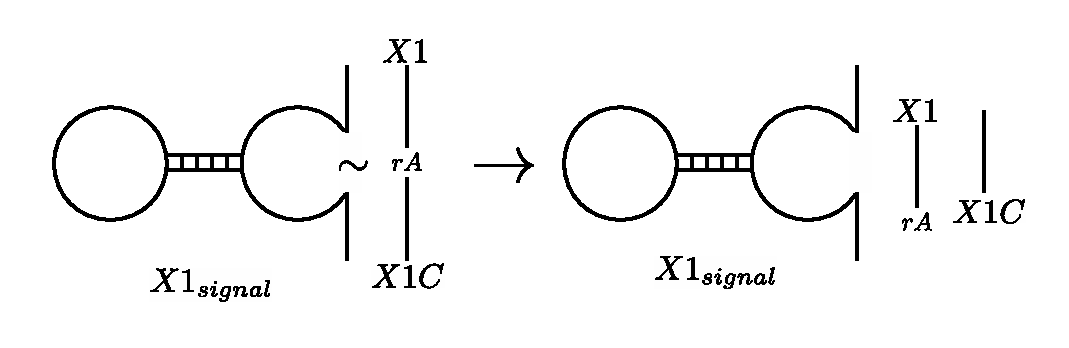
\includegraphics[width=12cm]{cleavage}
	\caption[Example of Deoxyribozyme Implementation]{Deoxyribozyme cascading example. Deoxyribozyme $X1_{signal}$ cleaves $X$ at embedded ribonucleotide ($rA$) to form $X1$ and $X1C$. A similar process occurs on $X1C$ to produce $X2$ and $X2C$.}
	\label{fig:deoxy1}
\end{figure}

We have discussed works operating typically on only a small region of \gls{dna} or representing only a few chemical reactions. The size of the system necessary to construct our full ant solver is much larger than these. For example, take the \gls{mdl} connected to the perceptrons in the previous chapter to form the \gls{ann} for our ant trail system. Each four- and five-input \gls{aasp} is composed of 33 and 38 reactions and 37 and 42 unique species, respectively. Recall from Chapter~\ref{chap:delay_line}, a four-input delay line requires eight reactions and 13 species. So, for an entire trail system with a hidden layer, this results in $8+33+3 \cdot 38=155$ reactions and $13+37+3 \cdot 42=176$ species for our system. This number of reactions and species is greater in complexity than other systems we have found presently implemented in a chemical system.

As an example, the four-neuron Hopfield associative memory from Qian \textit{et al.} contained around 160 reactions with 72 initial \gls{dna} species~\cite{Qian2011-nw}. While this system contained more reactions, the number of species co-existing in this system is less than half the number predicted for full computation of our trail system. One issue that Qian \textit{et al.} discuss in their work is that scaling up the system can amplify leak reactions that occurred and degrade performance of the overall system. Adding the increased number of species we require could have this type of issue. Another observation by Stojanovic and Stefanovic in their work was erroneous output by gates that should not be signalling. The authors mention that this behavior may lead to errors cascading in larger networks that may lead to undesired behavior~\cite{Stojanovic2003-eg}.

Taking a system, such as this today into a wet chemistry is not impossible, but perhaps difficult based on the current state of the art for the field. It seems that there is not a system of this scale presently implemented as a wet chemistry and other work by Qian \textit{et al.} mentions potential issues as their systems continued to grow in size. One area of improvement is perhaps looking at a way to reduce the complexity of the network in a \gls{crn}. With more work on complex network implementation in a \gls{crn}, in theory, it should be possible to map the trail system reactions with the methods used by Zhang and Seelig, Semenov \textit{et al.}, Stojanovic and Stefanovic, or Liu \textit{et al.} to a physical chemistry. Components of the system, like the delay line by itself, require a smaller number of reactions and may be more feasible for present implementation. If implemented in a wet chemistry, let us now discuss if we can predict the speed at which this system would operate based off current work.

\section{Processing Speed}
As discussed in the previous section, the applicable mapping of our work is likely the deoxyribozyme catalysis~\cite{Stojanovic2003-eg}~\cite{Stojanovic2000-qx}~\cite{Liu2009-jz}. Stojanovic and Stefanovic specifically find that 15 minutes is a reasonable time to cleave and accurately observe the results from the reactions in their tic-tac-toe system. The authors did observe that changing the size of the gates in the chemistry or the concentration of inputs did have an impact on the reaction time, but did not elaborate beyond that. Zhang and Seelig~\cite{Zhang2011-ey} also observe times in the scale of several minutes to compute similar systems in a \gls{dna} strand displacement model.

The advantage of the chemistry is the chemical reactions (for example, each calculation of output layer peceptron in our \gls{ann} controlling the ant) can occur in parallel. This of course assumes separation using the compartmental chemistry by Blount \textit{et al.}~\cite{Blount_undated-ro}. As an example, if we take the 15 minute time found by Stojanovic and Stefanovic per reaction, we can predict the cycle time for a single calculation in our trail system.

Let us start with the network in Figure~\ref{fig:chem_comp_dl4} and predict the time to complete a movement for the trail system. With a length four \gls{mdl}, that requires waiting on four steps to occur for shift and store the input value to each block of the delay line. Then, there is a required period of calculation at the hidden neuron followed by one in the output layer. The output layer perceptrons are all able to calculate their results in parallel unlike the delay line, which depends on previous inputs. 

So, in total, that gives six stages of calculation. With the 15 minutes found by Stojanovic and Stefanovic, that means approximately 90 minutes for a single calculation step for the full \gls{ann}. Running a full system with 200 steps of the John Muir trail would take approximately 12.5 days with this current technology. It is important to note as well that the time we are discussing here is the estimated time to reach a steady state. In a wet chemistry, all of the reactions are occurring in parallel, so a separation between the nodes represented in our \gls{ann} diagram is critical. 

Catalysts or other signaling methods are required to prevent the later nodes from consuming the species too early. For example in the delay line, we use our $Xn_{signal}$ species to perform this separation. Also, unlike in an electrical system, the inputs are consumed, meaning, that as we perform the calculation, we are actually decreasing the value of the input as the calculation occurs. 

Even though the value is over 12 days for this example, other architectures in chemistry may provide a faster run time. Kompa and Levine~\cite{Kompa2001-yk} discuss the use of different chemicals like aberchromes (I), fulgides, and merocyanines (II) that show dynamics faster than discussed from Stojanovic and Stefanovic. The authors even predict that with continued development of their work, it may be possible to see chemical reactions with photophysicochemical processes operating on a picosecond range.

\glsresetall
\chapter{Conclusion}
\label{chap:conclusion}
In this work, we have shown the feasibility of using \glspl{crn} as a means to implement control systems. We have demonstrated a partial solving of the Santa Fe trail in a \gls{crn}. We have also shown the ability of a \gls{crn} to partially navigate three sub-segments of the Santa Fe trail. We successfully navigate the easy Santa Fe trail easy segment consuming 100\% of the food. For the medium and hard segments and full Santa Fe trail, we are able to consume more than 44\% of the available food. This shows that it is possible to solve simpler versions of the trail without a need for \gls{ann} recurrence. Koza's genetic programs were able to consume all of the food on the Santa Fe trail. With further \gls{ga} optimization, \glspl{ann} in a \gls{crn} capable of consuming all food seems plausible.

We have also designed a flexible size memory necessary to provide storage for such control systems. The integration of our \gls{mdl} with the trail system \gls{ann} and \gls{asp} demonstrate the ability to hold values over time for later consumption by another system. With the \gls{bpl} delay line, we have shown the ability to learn 11 of the 14 linearly separable functions with an accuracy of greater than 85\%. Connecting these two delay line models with other systems also demonstrates the modular nature of the delay line system. A \gls{mdl} can precisely store values at the expense of manual signaling and our \gls{bpl} can do the same for smaller length memories without the need of manual control signaling.  Our \gls{mdl} also demonstrates a model capable of storing values with less than 0.01\% error.

\section{Contributions}
This work has made the following contributions to the field:
\begin{itemize}
\item a new type of memory implemented in a \acrlong{crn}, \acrlong{mdl}, in Chapter~\ref{chap:delay_line};
\item a new type of memory implemented in a \acrlong{crn}, \acrlong{bpl}, in Chapter~\ref{chap:delay_line};
\item the first chemical model capable of learning binary time series with the combination of the delay line and \acrlong{asp}, in Chapter~\ref{chap:delay_line};
\item a framework capable of simulating ant trail problems with user customizable parameters on \acrlong{ann} and \acrlong{ga} parameters, in Chapter~\ref{chap:trail_runner};
\item a web based application capable of navigating, filtering, and viewing data from simulations on ant trail problems with ease, in Chapter~\ref{chap:trail_runner};
\item a novel architecture with a single hidden perceptron for solving the ant trail problems with the addition of a delay line as a memory, in Chapter~\ref{chap:non_crn_testing};
\item an investigation into the minimal length of delay line length of four to solve the artificial ant problem in a non-\acrlong{crn} configuration, in Chapter~\ref{chap:non_crn_testing};
\item the first \acrlong{crn} implementation to solve the artificial ant problem, in Chapter~\ref{chap:trail_simulations};
\item the first \acrlong{ann} implemented in a \acrlong{crn} to compare system level functionality against other work, in Chapter~\ref{chap:trail_simulations};
\item evidence that a single hidden neuron when paired with a \acrlong{mdl} of length 4 is capable of solving 47\% of the John Muir trail, 44\% of the full Santa Fe trail, 100\% of the easy Santa Fe trail segment, 84\% of the medium Santa Fe trail segment, and 47\% of the hard Santa Fe trail segment, in Chapter~\ref{chap:trail_simulations};
\item proof that a \acrlong{ann} without a hidden neuron when paired with a \acrlong{mdl} of length 4 is capable of solving 47\% of the John Muir trail, 57\% of the full Santa Fe trail, 45\% of the easy Santa Fe trail segment, 84\% of the medium Santa Fe trail segment, and 47\% of the hard Santa Fe trail segment, in Chapter~\ref{chap:trail_simulations}.
\end{itemize}

\section{Future Work}
As discussed in Chapter~\ref{chap:trail_simulations}, the \gls{ga} used on \gls{crn} simulations was based off the \gls{ga} optimization performed in the non-\gls{crn} environment. Further optimization of the the \gls{ga} once the system is implemented as a \gls{crn} may yield better results for the overall system. The downside with such optimization is the long time to run simulations as discussed in Chapter~\ref{chap:trail_simulations}. As the speed to run the simulations decreases, such evaluations may be more feasible in the future. 

Banda has recently introduced a new type of delay line known as the parallel-accessible delay line~\cite{Banda2014-pf}. This delay line behaves similar to the \gls{mdl}, but adds a clock signal that does not require the manual signalling of the \gls{mdl}. The use of this delay line may in some instances reduce the complexity of the \gls{crn} reaction series.









%==============================================================================
%  Bibliography
%==============================================================================

\bibliographystyle{IEEEtran}
\bibliography{mainDoc}                  % bibliography file name mainDoc.bib  ------Neha (2010)

%==============================================================================
%  Appendices
%==============================================================================
\appendix

%==============================================================================
\end{document}
%==============================================================================
